\documentclass[a4paper,10pt,twoside,openright]{book}

\usepackage{libtex/algo}
\usepackage{libtex/thesisStyle}
\usepackage{graphicx, amssymb, amsmath, url, color, xcolor, booktabs, subfig, makeidx, tikz}
\usetikzlibrary{3d, positioning} 
\usetikzlibrary{shapes, arrows.meta, matrix, calc, decorations.pathreplacing, positioning, quotes} %ext.paths.ortho
\usetikzlibrary{positioning,fit,backgrounds,shadows}
\usetikzlibrary{shapes.multipart, decorations.pathmorphing}

\tikzset{>=latex} % for LaTeX arrow head
\colorlet{myred}{red!80!black}
\colorlet{myblue}{blue!80!black}
\colorlet{mygreen}{green!60!black}
\colorlet{mydarkred}{myred!40!black}
\colorlet{mydarkblue}{myblue!40!black}
\colorlet{mydarkgreen}{mygreen!40!black}
\tikzstyle{node}=[very thick,circle,draw=myblue,minimum size=22,inner sep=0.5,outer sep=0.6]
\tikzstyle{connect}=[->,thick,mydarkblue,shorten >=1]
\tikzset{ % node styles, numbered for easy mapping with \nstyle
  node 1/.style={node,mydarkgreen,draw=mygreen,fill=mygreen!25},
  node 2/.style={node,mydarkblue,draw=myblue,fill=myblue!20},
  node 3/.style={node,mydarkred,draw=myred,fill=myred!20},
}
\def\nstyle{int(\lay<\Nnodlen?min(2,\lay):3)} % map layer number onto 1, 2, or 3

\tikzset{
  level/.style={rectangle, draw=black, thick, minimum height=1cm, minimum width=5.5cm, align=center},
  arrow/.style={->, thick},
  labelbox/.style={rectangle, draw=none, align=left}
}

\usepackage[greek,english]{babel}
\usepackage[utf8]{inputenc}
\usepackage{pdfpages} % for \includepdf
\usepackage{caption}
\usepackage{lipsum} % for dummy text
\usepackage{multirow}
\usepackage{color} % colored links
\usepackage{hyperref} % for hyperlinks
\definecolor{deepblue}{RGB}{0,0,35} % quite a deep blue color

\hypersetup{
    colorlinks=true,
    linktoc=all,
    linkcolor=deepblue, % color of internal links
    citecolor=deepblue, % color of citations
    urlcolor=deepblue,  % color of URLs
}
\usepackage{algorithm}
\usepackage{algorithmic} % maybe use \usepackage{algpseudocode} sometime?
\usepackage{etoolbox} % for \ifnumcomp
\usepackage{listofitems} % for \readlist to create arrays
\usepackage{bbding}
\captionsetup{compatibility=false}

\usepackage{multicol} % for the multicol environment
\usepackage{bookmark}

\usepackage{natbib}
\bibliographystyle{plainnat}

% Title Page
\newcommand{\thesistitle}{Large Causal Models for AIOps}
%\newcommand{\thesistitlegreek}{}
\newcommand{\owner}{Nikolaos Kougioulis}
\newcommand{\firstprof}{Ioannis Tsamardinos}
\newcommand{\secondprof}{Sofia Triantafillou}
\newcommand{\thirdprof}{Professor 3}
\newcommand{\csdchair}{Professor 4}
\newcommand{\thesisdate}{\today}

\newtheorem{definition}{Definition}

\makeindex

\input{libtex/procs} % Procedural settings
\input{libtex/alias} % Alias and shorthand commands

\long\def\symbolfootnote[#1]#2
{\begingroup
	\def\thefootnote{\fnsymbol{footnote}}\footnote[#1]{#2}
	\endgroup}

\newcommand{\workperformedat}{\symbolfootnote[0]{This work has been performed at the University of Crete, School of Sciences and Engineering, Computer Science Department.}}
\newcommand{\worksupportedby}{\symbolfootnote[0]{The work has been supported by the Foundation for Research and Technology - Hellas (FORTH).}}

\makeatletter
\renewcommand{\@chapapp}{}% Not necessary...
\newenvironment{chapquote}[2][2em]
  {\setlength{\@tempdima}{#1}%
   \def\chapquote@author{#2}%
   \parshape 1 \@tempdima \dimexpr\textwidth-2\@tempdima\relax%
   \itshape}
  {\par\normalfont\hfill--\ \chapquote@author\hspace*{\@tempdima}\par\bigskip}
\makeatother

\begin{document}
	
	\begin{titlepage}
\begin{center}

    \Large \textbf{\thesistitle} \\[0.5cm]
    \Large \textit{\owner} \\[0.5cm]

    \vfill

    \normalsize{
    Thesis submitted in partial fulfillment of the requirements for the \\[0.30cm]
    \textit{Master of Science Degree in Computer Science and Engineering}} \\[0.30cm]

    University of Crete \\ School of Sciences and Engineering \\ Computer Science Department \\ Voutes University Campus, 700 13 Heraklion, Crete, Greece \\[0.5cm]

    \vfill

    \Large{Thesis Advisor: Prof. \firstprof} \\[0.5cm]

    \vfill

\end{center}

\workperformedat{} \worksupportedby{}

\end{titlepage}

	\begin{titlepage}
\begin{center}

    \textsc{University of Crete} \\
    \textsc{Computer Science Department} \\
    \vspace{0.4cm}
    \noindent {\textbf{\thesistitle}} \\
    \vspace{0.4cm}
    \noindent Thesis submitted by \\
    \textbf{\owner} \\
    in partial fulfillment of the requirements for the \\
    Masters' of Science degree in Computer Science \\
    \vspace{0.4cm} \textbf{THESIS APPROVAL} \\

    \vspace{0.4cm}

    \begin{tabular}{rl}
    Author: & \underline{\phantom{123456789012345678901234567890123456789012}}\\
    & \owner{}\\
    \\
    Committee approvals: & \underline{\phantom{123456789012345678901234567890123456789012}}\\
    & \firstprof{}\\
    & {\small Professor, Thesis Supervisor}\\
    \vspace{0.2cm}\\
    & \underline{\phantom{123456789012345678901234567890123456789012}}\\
    & \secondprof{}\\
    & {\small Professor, Committee Member}\\
    \vspace{0.2cm}\\
    & \underline{\phantom{123456789012345678901234567890123456789012}}\\
    & \thirdprof{}\\
    & {\small Professor, Committee Member}\\
    \vspace{0.2cm}\\
    Departmental approval: & \underline{\phantom{123456789012345678901234567890123456789012}}\\
    & \csdchair{}\\
    & {\small Assistant Professor, Director of Graduate Studies}\\
    \end{tabular}

    \vfill
    Heraklion, \thesisdate{}

\end{center}
\end{titlepage}

	\begin{titlepage}
    \begin{center}
        \Large \textbf{\thesistitle} \\[0.5cm]
        \large \textbf{Abstract} \\[0.5cm]
    \end{center}
    Causal discovery for both cross-sectional and temporal data has traditionally followed a dataset-specific paradigm, where a new model is fitted for each individual dataset. Such an approach underutilizes the potential of multi-dataset and large-scale pretraining, especially given recent advances in foundation models. The concept of \textit{Large Causal Models (LCMs)} envisions a class of pre-trained neural architectures specifically designed for temporal causal discovery. Existing approaches remain largely proofs of concept, typically constrained to small input sizes (e.g., five variables), with performance degrading rapidly to random guessing as the number of variables or model parameters increases. Moreover, current methods rely heavily on synthetic data, generated under arbitrary assumptions, which substantially limits their ability to generalize to realistic or out-of-distribution samples. This work addresses these challenges through novel methods for training on mixtures of synthetic and realistic data collections, enabling both higher input dimensionality and deeper architectures without loss of performance. Extensive experiments demonstrate that LCMs achieve competitive or superior performance compared to classical causal discovery algorithms, while maintaining robustness across diverse domains, especially on non-synthetic data cases. Our findings also highlight promising directions towards integrating interventional samples and domain knowledge, further advancing the development of foundation models for causal discovery.
    \vfill
\end{titlepage}
	%\begin{titlepage}
    \selectlanguage{greek}
    \begin{center}
        \Large \textbf{\thesistitlegreek} \\[0.5cm]
        \large \textbf{Περίληψη} \\[0.5cm]
    \end{center}
        \small{Η αιτιακή ανακάλυψη (\textlatin{Causal Discovery}), τόσο για συγχρονικά (\textlatin{cross-sectional}) όσο και για χρονικά (\textlatin{temporal}) δεδομένα, ακολούθησε παραδοσιακά ένα πρότυπο ειδικό στο εκάστοτε σύνολο δεδομένων (\textlatin{dataset-specific paradigm}), όπου ένα νέο μοντέλο εκτιμάται για κάθε μεμονωμένο, διαφορετικό σύνολο δεδομένων. Μια τέτοια προσέγγιση υποεκμεταλλεύεται τις δυνατότητες της προεκπαίδευσης πολλαπλών συνόλων δεδομένων και μεγάλης κλίμακας, ειδικά λαμβάνοντας υπ'όψιν των πρόσφατων εξελίξεων στα θεμελιώδη μοντέλα (\textlatin{Foundation Models}). Η έννοια των \textit{Μεγάλων Αιτιακών Μοντέλων (\textlatin{Large Causal Models})} οραματίζεται μια κατηγορία προ-εκπαιδευμένων νευρωνικών αρχιτεκτονικών (Θεμελιώδη Μοντέλα) ειδικά σχεδιασμένων για χρονική αιτιακή ανακάλυψη. Οι υπάρχουσες προσεγγίσεις παραμένουν σε μεγάλο βαθμό απλές επαληθεύσεις ιδεών, περιορισμένες σε μικρά μεγέθη εισόδου (π.χ., πέντε μεταβλητών), με την απόδοση να υποβαθμίζεται γρήγορα σε τυχαία εικασία καθώς αυξάνεται ο αριθμός των μεταβλητών ή των παραμέτρων του μοντέλου. Επιπλέον, οι τρέχουσες μέθοδοι βασίζονται έντονα σε περιορισμένο πλήθος αυθαίρετα παραγόμενων συνθετικών δεδομένων, γεγονός που περιορίζει σημαντικά την ικανότητά τους να γενικεύονται σε ρεαλιστικά ή εκτός κατανομής δεδομένα. Η παρούσα εργασία αντιμετωπίζει τις παραπάνω προκλήσεις μέσω νέων μεθόδων για εκπαίδευση σε μείξεις συνθετικών και ρεαλιστικών συλλογών δεδομένων, επιτρέποντας τόσο υψηλότερη διαστατιμότητα εισόδου όσο και βαθύτερες αρχιτεκτονικές χωρίς απώλεια απόδοσης. Εκτεταμένα πειράματα καταδεικνύουν πως τα Μεγάλα Αιτιακά Μοντέλα επιτυγχάνουν ανταγωνιστική ή ανώτερη απόδοση σε σύγκριση με κλασσικούς αλγόριθμους αιτιακής ανακάλυψης, διατηρώντας παράλληλα στιβαρότητα, ειδικά σε περιπτώσεις μη συνθετικών δεδομένων. Τα ευρήματά μας υπογραμμίζουν επίσης υποσχόμενες κατευθύνσεις προς την ενσωμάτωση παρεμβατικών δειγμάτων και εκ των προτέρω γνώσης, προωθώντας περαιτέρω την ανάπτυξη θεμελιωδών μοντέλων για αιτιακή ανακάλυψη.} \\[0.5cm]
    \selectlanguage{english}
    \vfill
\end{titlepage}
	
	\tableofcontents
	\listoftables
	\listoffigures

	%\chapter*{Preface}
\addcontentsline{toc}{chapter}{Preface}

\begin{chapquote}{Tao Te Ching, \textit{Lao Tzu}}
``A journey of a thousand miles begins with a single step.''
\end{chapquote}

This thesis marks the culmination of a long journey into the world of causality. The work presented was carried out in collaboration with the Foundation for Research and Technology Hellas in Heraklion and Huawei Ireland Research Centre in Dublin, Ireland. It represents part of a joint research project that brought together academic research and industrial perspectives on developing robust causal discovery methods under deep learning techniques, for real-world applications.

Writing this thesis has proven to be both a technical challenge and a personal journey, including multiple setbacks, experimental loops as well as positive surprises and breakthroughs. I hope that this work will not only contribute to advancing robust causal discovery methods for decision making, but also inspire further research in building machine learning systems that can reason about the world, instead of merely recognizing patterns.

\section*{Acknowledgements}

I would first like to thank my advisor for the guidance and pointers towards this work, on a novel line of research that was not without its own challenges and struggles. His vision and enthusiam has shaped much of this work. A special thanks goes to Dr. Nikolaos Gkorgkolis, as both a collaborator and postdoctoral mentor, whose insight and enthusiasm for scientific discovery have shaped much of this work. I am grateful for our thoughtful discussions, creative ideas, countless meetings, software engineering, research writing and planning. I also want to thank all the members of the AIOps team at Huawei Ireland Research Centre: Wang MingXue, who led this collaboration; Bora Caglayan, Andrea Tonon and Dario Simionato, for bridging the gap between the two teams with patience. Working with such talented people has been a rewarding aspect of this journey. Finally, I want to express my deepest gratitude to my family for their unwavering love and encouragement. This includes my mother Sofia, my father Michalis and my brother Christos. Nothing in my life would have been possible without them.

\section*{Publications}

This thesis is based upon the following papers:

\begin{enumerate}
    \item \textit{Temporal Causal-based Simulation for Realistic Time-Series Generation} \\
          Nikolaos Gkorgkolis$^*$, \underline{Nikolaos Kougioulis}$^*$, MingXue Wang, Bora Caglayan, Andrea Tonon, Dario Simionato \& Ioannis Tsamardinos \\
          (ArXiv Preprint: arXiv:2025.01.01)

    \item \textit{Large Causal Models for Temporal Causal Discovery} \\
          \underline{Nikolaos Kougioulis}, Nikolaos Gkorgkolis, MingXue Wang, Bora Caglayan, Andrea Tonon, Dario Simionato \& Ioannis Tsamardinos \\
          (In preparation)
\end{enumerate}

\def\thefootnote{*}\footnotetext{Authors contributed equally to this work.}\def\thefootnote{\arabic{footnote}}

%The following works, although not an integral work of this thesis, were also completed during its preparation.

%\begin{enumerate}
%    \item ...
%\end{enumerate}
	%\chapter{Introduction}\label{chap:introduction}

\begin{chapquote}{Alice in Wonderland, \textit{Lewis Carroll}}
``Begin at the beginning, the King said, very gravely, and go on till you come to the end: then stop.''
\end{chapquote}

\section{The Setting} \label{sec:setting}

Modern data engineering and analysis techniques, spanning fields from classic statistics to medical research, rely heavily on predictive modeling. They revolve around examining observed datasets and building predictive models on outcomes of interest, based on a set of predictive features. A fundamental limitation of predictive models is their inability to capture the underlying generative mechanisms driving the relationships between the observed variables, relying purely on correlation statistics from observational data.

The well-known adage, \textit{Correlation does not imply causation}, exemplifies the fundamental challenge of causality, highlighting the need to move beyond predictive modeling and embrace causal reasoning. Importantly, the understanding of causal relationships is essential for answering “what-if” and “why” questions that go beyond mere prediction and association. In domains such as healthcare and climate change, one needs to know how an intervention (a change of the internal mechanisms of the examined system) will affect an outcome of interest, or even why a particular outcome occurred under certain observed conditions. In the end, for classical statistical and machine learning (ML) models, it all boils down to leveraging large portions of associational information and past experience from observational data, in order to construct, informally speaking, a pattern recognition system. 

Although so far in history predictive models have proven more than adequately robust for a wide range of applications, distributions of samples are assumed to be independent and identically distributed (i.i.d.), thus drawn from a single, unchanged distribution (samples are obtained under the same, unaltered experimental scenarios). What's more, understanding the underlying mechanism between cause and effect enables causal models to cover a wide range of distributions: By altering experimental conditions with interventions, one is able to uncover the true propagation of causation and perform reliable predictions under environmental changes. On the contrary, although statistical models have been proven robust for a variety of applications, they only account for modeling one general population distribution and are thus less interpretable. 

As an example, consider predicting ice cream sales based on the number of sunburn cases in a country. There clearly exists a correlation between these two observed quantities, so one may construct a model to predict ice cream sales based on its linear or non-linear relationship with sunburn cases. However, we generally know (taking it as expert knowledge) that the number of sunburn cases is not a cause of ice cream sales, but rather a result of the sun's radiation in the summer period. Allowing some gentle introduction to the appropriate terminology and notation, we qualitatively represent causal relationships of an underlying system using \textit{Directed Acyclic Graphs (DAGs)}\footnote{Other graphical structures exist, but are outside the scope of this work.}, where observed variables are depicted nodes and a directed edge \( X \rightarrow Y\) is interpreted as "\(X\) is a direct cause of \(Y\)" , while "\(Y\) a direct effect of \(X\)". With this in mind, the causal DAG described before is \(\text{Sun Radiation} \rightarrow Ice Cream Sales\) and \(\text{Sun Radiation} \rightarrow \text{Sunburn Cases}\).


Now imagine an alternate reality where the whole population is educated such that everyone applies adequate sunscreen before heading to the beach during summer. Using a model that performs its prediction trained on the false relationship discussed earlier in this modified population environment is guaranteed to produce highly inaccurate outcomes. This problematic case lies in the presence of the \textit{unobserved (latent) confounding variable} \( \text{Sun Radiation} \), which causally influences both \(\text{Sunburn Cases} \) and \( \text{Ice Cream Sales} \) (its direct children in the causal DAG). More often than not, creating a model that accounts for all possible eventualities is either impossible or intractable due to time or moral constraints. Of course, not all domains have been hindered by the observations we outlined, such as natural language processing (NLP), which has seen remarkable progress in recent years. Yet, our discussion so far further highlights the need for incorporating causality-based methods in machine learning algorithms to obtain a deeper understanding of examined systems. As \citet{scholkopf2021towards} point out: \\

\begin{chapquote}{\citet{scholkopf2021towards}}
``If we wish to incorporate learning algorithms into human decision making, we need to trust that the predictions of the algorithm will remain valid if the experimental conditions are changed.''
\end{chapquote}

As Reichenbach points out in the \textit{common cause principle} \citep{reichenbach1956direction}, if two variables \(X\) and \(Y\) are statistically dependent, then either (i) \(X\) causes \( Y\), (ii) \(Y\) causes \(X\) or importantly (iii) \textit{they share a common cause \(Z\) (a confounder \(X \leftarrow Z \rightarrow Y\)) that explains their association}. This principle lies at the heart of why observational data can be misleading: without accounting for all relevant variables, we risk attributing causal meaning to mere correlations. A classic illustration of this issue is \textit{Simpson's Paradox} \citep{simpson1951interpretation}, where trends apparent in aggregated data are reversed when disaggregated by a confounding variable. For instance, a treatment might appear beneficial in both men and women when analyzed separately, yet detrimental when the data is pooled together, due to the unequal distribution of underlying risk factors (e.g. a factor prominent in women).

Additionally, modern machine learning tools such as \textit{feature importance scores} and \textit{Shapley (SHAP) values} \citep{lundberg2017unified} often provide insights into which variables most strongly influence a prediction. Unfortunately, these measures are fundamentally \textit{associational} and non-causal: they capture how much a feature contributes to predictive accuracy within the model, but not whether the feature exerts a causal effect on the outcome. Consequently, they remain vulnerable to the same confounding phenomena highlighted previously: A variable may appear to have high importance or a strong SHAP attribution simply because it is correlated with an unobserved cause, rather than because it directly drives the outcome.

\begin{table}[ht!]
\centering
\caption{Comparison of different types of causal queries.}
\label{tab:causal-query-comparison}
\renewcommand{\arraystretch}{1.4}
\small
\begin{tabular}{|p{2.5cm}|p{2.5cm}|p{4cm}|p{2.5cm}|}
\hline
\textbf{Type} & \textbf{Notation} & \textbf{Interpretation} & \textbf{Data Source} \\
\hline
\textbf{Observational} & \( \mathbb{P}(Y \mid X=x) \) & How does \(Y\) vary when we observe \(X=x\)? & Observational \\
\hline
\textbf{Interventional} & \( \mathbb{P}(Y \mid \mathrm{do}(X=x)) \) & What happens to \(Y\) if we intervene and set \(X=x\)? & Interventional (RCTs, simulations) \\
\hline
\textbf{Counterfactual} & \( \mathbb{P}(Y_{X = x'} \mid X=x, Y=y, Z=z) \) & What would \(Y\) have been if \(X = x'\), given we saw \(X=x, Y=y, Z=z\)? & Model-based (SCMs + Abduction) \\
\hline
\end{tabular}
\end{table}

Given our discussion so far, how would one proceed to measure causal effects correctly? The gold standard since its introduction by Ronald Fisher \citep{fisher1935design}, has been with randomized experiments and more specifically with \textit{Randomized Control Trials (RCTs)}, where a subset of the examined population is randomly split into \textit{control} and \textit{treatment} groups, where one more more variables are deliberately manipulated (intervened) to isolate the causal effects being measured. As an illustrative example, consider a clinical trial where one needs to decide whether the newly introduced pill \(X\) prevents migraines. An RCT experiment would imply selecting a random patient sample, randomly splitting them into control (placebo pill) and treatment (pill \(X\)) groups and measure the causal effect of a quantity of interest (e.g. migraine pain level) on each group separately. The real magic of such controlled experiments lie in their ability to eliminate \textit{confounding bias} through randomization. By balancing both observed and unobserved covariates across groups, RCTs ensure that differences in outcomes are attributed solely to the intervention and not to systematic distortions caused by pre-existing conditions. In digital marketing and advertising campaigns, RCTs take the form of \textit{A/B tests}: users are randomly shown one of two versions of a webpage or a smartphone app (A or B) to determine which version has a greater causal effect on a desired outcome, such as \textit{click-through rate} or \textit{exposure rate} for a quantity of interest. Returning to our earlier ice cream and sunburn example, one would randomly assign a subset of the population to consume ice-cream (treatment group) and another to not (control group) and measure the causal effect of ice-cream consumption on sunburn cases. In formal terms, such a measurement can for example be the \textit{Average Treatment Effect (ATE)}, which is viewed as the expected difference in outcomes between treated and untreated populations: \(\text{ATE} = \mathbb{E}[Y_1 - Y_0]\) where \(Y_1\) and \(Y_0\) represent the potential outcomes under treatment and control, respectively. If this difference is statistically distinguishable from zero, one concludes that the treatment has a causal effect on the outcome.

However, controlled experiments like RCTs are often impractical due to cost, ethical constraints or logistical challenges, with many corporations running hundreds of them each day on their products. For instance, it would be prohibitive to force a population sample (including healthy individuals) to smoke for investigating whether smoking causes lung cancer. What is more, the space of possible A/B tests is combinatorial when one is considering combinations of several design choices or user behaviors, thus being unfeasible in practice. 

\begin{figure}[ht!]
\centering
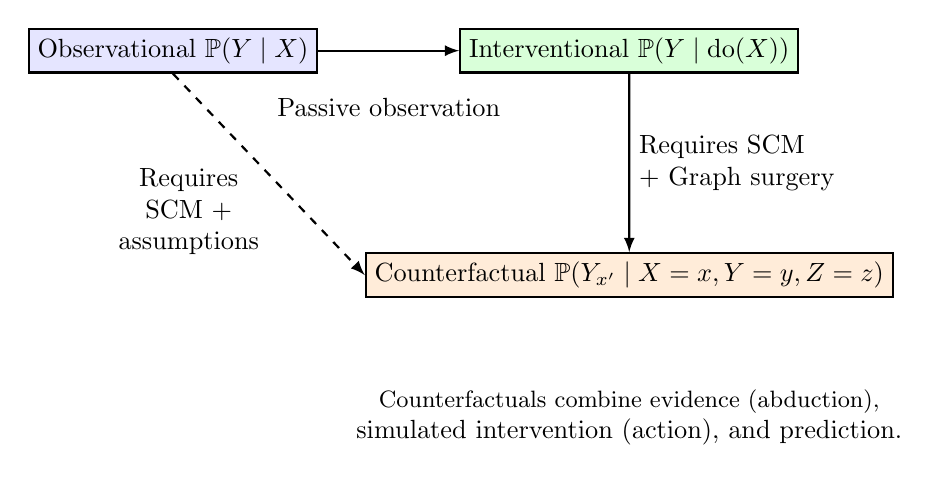
\begin{tikzpicture}[node distance=1.8cm, thick, every node/.style={scale=0.95}]
  % Nodes
  \node[draw, rectangle, fill=blue!10] (obs) {Observational \(\mathbb{P}(Y \mid X)\)};
  \node[draw, rectangle, fill=green!15, right of=obs, xshift=4.3cm] (intv) {Interventional \(\mathbb{P}(Y \mid \mathrm{do}(X))\)};
  \node[draw, rectangle, fill=orange!15, below of=intv, yshift=-1.2cm] (cf) {Counterfactual \(\mathbb{P}(Y_{x'} \mid X=x, Y=y, Z=z)\)};

  % Arrows
  \draw[->] (obs) -- node[below, yshift=-0.5cm] {Passive observation} (intv);
  \draw[->] (intv) -- node[right, align=left] {Requires SCM\\ + Graph surgery} (cf);
  \draw[->, dashed] (obs.south) -- node[left, align=center, yshift=-0.5cm] {Requires \\ SCM + \\ assumptions} (cf.west);

  % Labels
  \node[below of=cf, yshift=-0.1cm, align=center] (note) {\small Counterfactuals combine evidence (abduction),\\ simulated intervention (action), and prediction.};
\end{tikzpicture}
\caption{Illustration of the relationships and requirements between observational, interventional, and counterfactual causal queries.}
\label{fig:causal-query-flow}
\end{figure}

This is where the formal framework of \textit{Structural Causal Models (SCMs)} becomes essential. SCMs, introduced by Judea Pearl \citep{pearl2009causality} who pioneered the development of the theory of Causality (Turing Award 2011), offer a mathematical representation of the causal mechanisms that generate a dataset. In brief, an SCM consists of (i) a graph (in this text, a DAG) \(\mathcal{G}\) structure encoding the underlying causal relationships (ii) a set of structural equations (functional relationships) \( X_i := f_i (\text{Pa}_i, \epsilon_i)\) where \(\text{Pa}_i\) are the parents of \(X_i\) in the DAG and (iii) independent noise terms \(\epsilon_i\) representing unobserved randomness and possible confounders. In a nutshell, these structural equations \textit{encapsulate how each variable in a system is generated from its direct causes (parents in the DAG)}. The strength of such modeling lies in the ability to rigorously represent the causal mechanisms that generate a dataset, enabling the analysis of causal effects and interventions, and the estimation of causal quantities of interest, such as the ATE mentioned previously.

Furthermore, the concept of interventions is a fundamental operation in causal inference, formalized through \textit{do-calculus} by Pearl \citep{pearl1995causal}. The notation \(\mathbb{P}(Y|\text{do}(X=x))\) denotes the distribution of \(Y\) after an intervention on \(X\), directly setting its value to \(x\), irrespective of its natural causes. Such generated datasamples are called \textit{interventional data} in contrast to \textit{observational data} that are obtained from a purely observational perspective of the system. In terms of the SCM, this corresponds to \textit{graph surgery}: removing all incoming edges into \(X\) and replacing its value with a constant. This operation gives rise to a new graph, called the \textit{mutilated graph}, which simulates a world where we have forced \(X\) to be \(x\). This distinction is crucial because in observational data, one only has access to the conditional observational distribution \(\mathbb{P}(Y|X=x)\) which may be influenced by confounding or selection bias. On the other hand, the interventional distribution \(\mathbb{P}(Y|\text{do}(X=x))\) truly captures the causal effect of manipulating \(X\) on \(Y\). So generally, the interested reader may notice that \(\mathbb{P}(Y|X=x)\) (which may represent the outcome of a predictive model) is generally not equal to \( \mathbb{P}(Y|\text{do}(X=x))\)\footnote{They would be equal in the case of no backdoor-confounding path from \(X\) to \(Y\), but this is outside the scope of this thesis.}. Finally, a third important pillar in Causality is the concept of \textit{counterfactuals}, where one can quantify causal queries of the form \textit{"Given that I have observed \(X=0,Y=0\) and \(Z=1\), what would \(Y\) be if \(Z\) had been \(0\)?"}. That is, a counterfactual probability of the form \( \mathbb{P}(Y_{Z=0}=y|X=0, Y=0, Z=1)\). Computation of such queries is evaluated with a three-step procedure known as \textit{abduction}, \textit{action}, and \textit{prediction} using the known SCM \citep{pearl2009causality}. Here, \(Y_{Z=0}\) denotes the potential outcome representing the value that \(Y\) would have taken, in a reality where \(Z=1,X=0\) and \(Y=0\) have been observed. One concrete example of counterfactuals is: "Knowing that Hillary Clinton gave a speech in California and did not win the 2016 presidential election, would she had won had she not given that speech?". Unlike predictive explanations, which are conditional on inputs, counterfactuals model alternative realities rooted deeply in the structural model of the world, essential for decision-making under uncertainty and policy evaluation. Figure \ref{fig:causal-query-flow} and Table \ref{tab:causal-query-comparison} provides an overview of the causal queries discussed so far. 

In ML literature, one also encounters \textit{counterfactual explanations (CFEs)} \citep{guidotti2024counterfactual} which are commonly used as interpretability tools. These CFEs typically answer queries of the form "What minimal change in the input features would have altered the model's prediction?". One must note that they are not counterfactuals in the causal sense: they operate within the predictive model's input-output mapping, without assuming any underlying structural causal model. As a result, suggested changes may be infeasible, non-actionable, or causally meaningless. Table \ref{tab:causal-vs-predictive} provides an overview of the differences discussed between causal and predictive modeling.

\begin{table}[h!]
\centering
\renewcommand{\arraystretch}{1.2}
\begin{tabular}{|p{2.5cm}|p{5cm}|p{3cm}|p{3cm}|}
\hline
\textbf{Query} & \textbf{Description} & \textbf{Causal} & \textbf{Predictive} \\
\hline
Prediction & Predict/Diagnose $Y$ given $X$ & Correct predictions & Correct predictions \\
\hline
What-if & What if I set \(X_1=5\) ? & Correct prediction on $Y$ & Possibly wrong prediction on $Y$ \\
\hline
Decision Making & Optimal \(X_1\) to increase \(Y\) given \(X_2=6\) & Correct decisions & Possibly wrong decisions \\
\hline
Interpretation & Importance of \(X_1\) in affecting \(Y\); features influencing \(Y\) & Correct estimate & SHAP/feature importance may fail \\
\hline
Counterfactual & Example: \(Y=3\) when \(X_3=\) ``yellow''. What if \(X_3=\) ``green''? & Correct estimate & Not possible \\
\hline
Root Cause & What was the initial root cause of a failure? & Correct estimate & Possibly wrong estimates \\
\hline
\end{tabular}
\caption{Comparison of causal vs. predictive modeling across different types of queries.}
\label{tab:causal-vs-predictive}
\end{table}

All the above positive baggage of the theory of Causality is described by Judea Pearl in the \textit{3-step ladder of Causation} \citep{pearl2018book}. Any inference merely by observing associations lies in \textit{level 0} (as in statistical predictive models). The true power of causality belongs to interventions (\textit{level 1}) and counterfactuals (\textit{level 2}). From everyday choices to scientific inquiry, our actions are guided by the belief that certain causes will lead to specific effects. However, causality in real-world scenarios is often probabilistic rather than deterministic. As we have mentioned before, while smoking is a known cause of lung cancer, not all smokers develop the disease. This uncertainty is also where probability theory intersects with causal modeling, allowing us to quantify the likelihood of outcomes given specific causes.

%\begin{figure}[t!]
%\centering
%\begin{tikzpicture}[node distance=1.9cm]
%
%% Levels
%\node (seeing) [level] {Association (Seeing, Observing) \\ \(\mathbb{P}(Y \mid X)\)};
%\node (doing) [level, above=of seeing] {Interventions (Doing) \\ \(\mathbb{P}(Y \mid \mathrm{do}(X))\)};
%\node (imagining) [level, above=of doing] {Counterfactuals (Imagining, \textit{What if...}) \\ \( \mathbb{P}(Y_{x'} \mid X = x, Y = y, Z = z)\)};
%
%% Arrows
%\draw [arrow] (seeing) -- (doing);
%\draw [arrow] (doing) -- (imagining);
%
%% Labels
%\node [labelbox, right=0.6cm of seeing] {Observational ~Data};
%\node [labelbox, right=0.6cm of doing] {Interventional ~Data};
%\node [labelbox, right=0.6cm of imagining] {Abduction + SCM};
%
%\end{tikzpicture}
%\caption{Depiction of Pearl's Ladder of Causation, progressing from association (level 0) to intervention (level 1) and finally to counterfactual reasoning (level 2).}
%\label{fig:ladder-of-causation}
%\end{figure}

Overall, Causality can be split into two main research areas: \textit{causal discovery (CD)}, which aims to identify the true underlying causal relationships from data under certain assumptions and \textit{causal inference (CI)}, which concerns estimation and quantification of treatment effects without exhaustive experimentation. Formally, given a dataset \( \mathcal{D} \sim \mathcal{P}_{\mathcal{D}} \), the goal of causal discovery is to infer the underlying causal model \( \mathcal{G} \sim \mathcal{D} \). Methods developed for causal inference assume the ground truth causal structure as known. In practice, one starts by estimating the ground truth causal model using a causal discovery algorithm. Depending on the method, the discovered causal model may be paired with the estimated functional dependencies of the underlying SCM (e.g. some algorithms assume that data follow a linear generative process, so causal discovery is reduced to estimating the coefficients of the assumed linear model) or simply output the estimated DAG. In either case, one can use standard predictive models to estimate the functional relationships alongside valid adjustment sets to perform causal inference. This bridges causal discovery with interventional effect estimation: identifying optimal intervention strategies, computing ATEs, or performing counterfactual reasoning on outcomes of interest, as described previously. 

In recent years, significant attention has shifted on \textit{causal discovery for time-series (temporal) data} \citep{runge2018causal, runge2019inferring, runge2023causal}. For the unfamiliar reader, such samples are no longer considered i.i.d. as the time dimension is also present. Time-series are widely observed across a domain of environments, as long as data is collected across time intervals and exhibit a temporal order. For example, consider a time series of climate measurements (temperature, humidity, atmospheric pressure) over a day in a city, sampled every fifteen minutes. The resulting data is a sequence of three-dimensional 96 observations, and the corresponding (multivariate) time series is a time-series of length 96. Another concrete example would be a time series of stock prices, where data is collected every day for a year, resulting in a time series of length 365. For the most part, investigating causality for time-series consists as an extension of the theory developed for the static, i.i.d. counterparts, with some additional assumptions and complexities that arise from temporal dependencies, possible feedback loops, non-stationarity of the observed time-series, and unobserved confounding variables. Variables evolve over time, and causal influences can occur both contemporaneously (within the same time-index) and with various time lags (e.g. one day before). Without elaborating extensively in this part of the text, a \textit{contemporaneous} (or \textit{instantaneous}) relationship may occur if causal effects exist within an hourly period in an observed daily time-series. 

Concurrently and much to our benefit, there has been no previous period for ML and artificial intelligence (AI) with as much bloom and research opportunities. The current wave of interest, initiated with ML more than two decades ago and continued with \textit{deep learning (DL)} (the use of large neural network architectures for solving highly-complex, intractable tasks) has provided several radical solutions to numerous research questions, such as image recognition, that no previous AI period ever did. The witnessing of problems that have puzzled the scientific community for decades being deemed solved, like text-to-image generation, is an ongoing process. It is possible that since this ongoing take-off, the AI winter may not be coming anytime soon. 

Even more remarkably, causality for time-series data has only recently found large-scale applications in industrial domains, many years after Pearl's seminal contributions. Terms such as \textit{Causal AIOps} and \textit{Causal AI} correspond to complementing traditional machine learning with causal discovery \& causal inference methods, often based around modern neural architectures for industrial applications. Much to our excitement, \textit{Causal Digital Twins} \citep{jakovljevic2021towards} are also a promising direction, where a causal model is constructed from data to model a real-world system, to perform real-time causal inference and decision making. This enables tasks such as the identification of optimal interventional policies, which are crucial for understanding and correctly interpreting data-driven decisions. This paves exciting research paths for developing new state-of-the-art (SOTA) methods for causality on time-series for solving real-world problems.

\section{Motivation} \label{sec:motivation}

The field of causal discovery has undergone an important paradigm shift with the introduction of deep learning-based approaches. A landmark contribution is the NOTEARS paper by \citet{zheng2018dags}, which recast causal discovery as a continuous optimization scheme with acyclicity constraint, by relaxing the combinatorial nature of the problem. This opened the door to a whole class of differentiable causal discovery methods. In the i.i.d. setting, this led to the introduction of works such as DECI \citep{geffner2024deep}, AVICI \citep{lorch2022amortized} and CSIvA \citep{ke2023learning}, which leverage modern deep neural architectures and approaches to infer causal structure from data. Various works for temporal (time-series) data soon followed, with methods such as TCDF \citep{nauta2019causal}, ACD \citep{lowe2022amortized} and Rhino \citep{gong2023rhino} among others. \citet{assaad2022survey} and \citet{deng2022deep} provide a self-contained review on works for temporal causal discovery, for the interested reader.

Despite their promise, existing approaches face a number of limitations. Classical causal discovery methods for time-series based on conditional independence testing, such as PCMCI \citep{runge2018causal}, suffer from scalability issues due to the exponential number of independence tests required. While these methods are provably sound if infinite sample size is available \citep{spirtes2001causation}, they often fail to generalize in reduced, finite-sample regimes. Score-based methods, which search over graph structures using data likelihood or other criteria, such as DYNOTEARS \citep{pamfil2020dynotears}, can underperform when functional dependencies are complex or nonlinear, on the advantage of faster convergence (as linearity of causal relationships is assumed). Importantly, all of these methods operate on a single input-output pair at a time, which limits their ability to learn from multiple samples and causal graphs of varying sizes, complexities and dynamics. As a result, the challenge of building causal discovery methods that generalize across data distributions and promise high scalability to realistic time-series scenarios remains unresolved.

Meanwhile, the rise of \textit{foundation models} has revolutionized several domains of machine learning. In a nutshell, a foundation model (FM) refers to a pre-trained neural model, trained on large corpuses of data \citep{bommasani2021opportunities}. In natural language processing, the introduction of BERT \citep{devlin2019bert} marked a turning point by demonstrating the power of pretraining Transformer-based \citep{vaswani2017attention} models on massive data corpora, in the context of text translation. Previous works, being reliant on recurrent neural networks (RNNs), have been proven limited by design, in contrast to the Transformer architecture which has efficiently transformed the field of NLP. This was followed by the GPT family, culminating in models like GPT-4 \citep{achiam2023gpt}, which use hundreds of billions of parameters to support robust zero-shot\footnote{The ability of a model to generalize to data that has not been included in training, i.e. does not follow the distribution of the training data.} generalization \citep{radford2018improving, radford2019language}. Foundation models have also emerged in vision and multimodal learning, e.g. CLIP \citep{radford2021learning} and DALL-E \citep{ramesh2021zero}, exhibiting remarkable generalization across diverse downstream tasks. A unifying principle behind these models is that \textit{massive pretraining on varied data can lead to robust representations and inference capabilities without any task-specific supervision}. Recent work has extended this idea to time-series forecasting. Models such as TiMeR and TiMeR-XL \citep{liu2024timer} adopt decoder-only Transformer architectures to autoregressively model temporal sequences. MOIRAI \citep{woo2024unified} uses a masked encoder and patch-based input for forecasting, with model sizes ranging from 14M to 311M parameters. Google's TimesFM \citep{das2024decoder} follows a similar patch-based decoder design, with a 200M parameter footprint. These models demonstrate strong \textit{out-of-distribution (OOD)}\footnote{Performance on datasets that do not follow the distribution of the training data, also known as \textit{zero-shot} in the context of foundation models.} forecasting capabilities, suggesting that general-purpose foundation models for temporal data are viable. An overview of these foundation models, along with their sizes, is shown in Table \ref{tab:model-sizes}. 
 
\begin{table}[ht!]
\centering
\caption{Comparison of foundation model sizes across NLP and time-series forecasting domains.}
\label{tab:model-sizes}
\renewcommand{\arraystretch}{1.3}
\small
\begin{tabular}{|l|c|c|}
\hline
\textbf{Model} & \textbf{Domain} & \textbf{Parameters} \\
\hline
BERT \citep{devlin2019bert} \scriptsize{(Base)} & NLP & 108M \\
GPT-1 & NLP & 117M \\
%GPT-3.5 & NLP & 175B \\
%GPT-4 (est.) & NLP & \(\sim\)1.7T \\
\hline
Timer \citep{liu2024timer} & Time-series Forecasting & 84M\footnote{Model weights available at \url{https://huggingface.co/thuml/timer-base-84m}.} \\
MOIRAI \scriptsize{(Small / Base / Large)} \citep{woo2024unified} & Time-series Forecasting & 14M / 91M / 311M \\
TimesFM \citep{das2024decoder} & Time-series Forecasting & 200M\footnote{Model weights available at \url{https://huggingface.co/google/timesfm-1.0-200m}.} \\
\hline
\end{tabular}
\end{table}

Our work aims to extend this line of research towards causal discovery for time-series data. The concept of \textit{Large Causal Models (LCMs)} envisions a class of deep, pre-trained neural architectures specifically designed for temporal causal discovery. These models are trained on a diverse corpus of multivariate time-series sequences, paired with their corresponding ground-truth structural causal models, with a single aim: \textit{learning robust universal representations capable of performing zero-shot temporal causal discovery with refined lag estimation from arbitrary time-series samples} (Figure \ref{fig:lcm-goal}).

Unlike existing temporal state-of-the-art methods, which are often constrained to small numbers of variables and suffer from significant performance degradation as input dimensionality and model size increases, we showcase robust generalization of our LCMs across varying numbers of variables, time-series lengths, and temporal dynamics. By leveraging both synthetic and \textit{simulated} (realistically generated) datasets, our models aim to capture universal causal structures that are robust across domains, time scales, and data distributions. Moreover, causal discovery using LCMs is performed via a single forward pass over input data, making it significantly faster and scalable than traditional approaches, opening the door for real-time applications such as causal digital twins for decision-making and control.

Constructing foundation models for causal discovery raises several central challenges. First, input dimensionality (as in all pre-trained models) must be carefully considered: the maximum number of variables and timesteps directly impacts both feasibility and generalization. Inputs that are too small limit applicability, while overly large inputs may hurt performance. Second, training data quality and diversity are crucial. While existing approaches rely solely on synthetic data generated from arbitrary SCMs \citep{stein2024embracing}, purely synthetic datasets fail to capture the full complexity of real-world processes. To make matters worse, the availability of ground-truth causal structures from the real-world is scarce to non-existent. \textit{Semi-synthetic data}, based on existing knowledge of real scenarios (such as physical models or approximations of them by stochastic dynamical systems) can offer a pragmatic compromise, but a principled methodology for generating high-quality, diverse, and realistic SCM time-series pairs at scale remains a key open challenge; one which we address in Chapter \ref{chap:data}.

\begin{figure}[ht!]
\centering
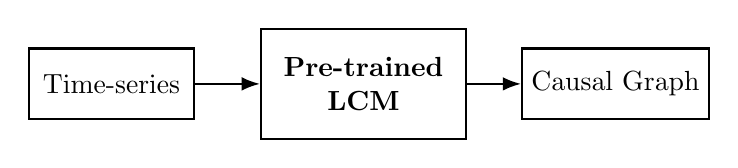
\begin{tikzpicture}[>=Latex,thick]
  % Nodes (absolute, compact layout)
  \node[draw, align=center, minimum width=2.1cm, minimum height=0.9cm] (in)  at (0,0) {Time-series};
  \node[draw, align=center, minimum width=2.6cm, minimum height=1.4cm] (lcm) at (3.2,0) {\textbf{Pre-trained}\\ \textbf{LCM}};
  \node[draw, align=center, minimum width=2.1cm, minimum height=0.9cm] (out) at (6.4,0) {Causal Graph};

  % Arrows
  \draw[->] (in) -- (lcm);
  \draw[->] (lcm) -- (out);
\end{tikzpicture}
\caption{A pre-trained Large Causal Model (LCM) infers a causal graph from an unknown time-series data sequence. (Training uses thousands of pairs of time-series and their corresponding ground-truth causal graphs.)}
\label{fig:lcm-goal}
\end{figure}

\section{Related Work} \label{sec:related-work}

This section provides an overview of recent work connecting causality with deep learning, focusing particularly on attention-based and foundation-model approaches. We highlight methods not only on causal discovery but also on causal inference, as they provide valuable insights for our own work. 

\subsection{Causal Inference with Attention}

The integration of causal inference into deep learning models remains relatively nascent. One notable effort is \textit{Causal Inference with Attention (CIvA)} by \citet{zhang2023towards}, which introduces a self-supervised transformer-based architecture for estimating Average Treatment Effects (ATEs) from observational data. Their approach leverages a primal-dual link between covariate balancing and self-attention, enabling the model to generalize under moderate shifts in causal mechanisms. While effective for ATE estimation, CInA is not designed for causal graph discovery and does not address temporal data.

\subsection{Do-PFN}

A very recent advancement in causal inference is \textit{Do--PFN} by \citet{robertson2025do}, which adapts Prior-data Fitted Networks (PFNs) for causal effect estimation. Rather than discovering the causal structure, Do--PFN focuses on learning to predict interventional outcomes (i.e., conditional interventional distributions, or CIDs) directly from observational data. The model is pre-trained on millions of synthetic datasets derived from randomly sampled SCMs, learning a meta-model capable of in-context causal inference without requiring knowledge of the ground-truth causal graph. While Do-PFN demonstrates impressive performance in both synthetic and semi-real evaluations, including frontdoor and backdoor adjustment cases, it is limited to point estimation tasks such as CID or CATE prediction. Importantly, Do--PFN does not attempt to recover or represent the underlying causal graph or temporal dynamics, which makes it orthogonal to our objective of structure discovery. Moreover, Do-PFN operates on i.i.d. tabular data and does not consider multivariate time-series or lagged causal dependencies. It also scales to graphs up to 10 nodes and degrades with noise, yet improves with dataset size. Do--PFN uses an explicit prior over SCMs and amortizes inference across them. It also captures uncertainty due to unidentifiability, i.e., integrating over model priors.

\subsection{Sample, Estimate, Aggregate}

In the causal discovery domain, \citet{wu2024sample} propose a method that aggregates subgraph-level causal estimates using axial attention alongside global statistical features such as inverse covariance. Although innovative, their method is limited to static (i.i.d.) data and does not extend to time-series or interventional settings. 

\subsection{CSIvA}

Similarly, \citet{ke2023learning} (with \textit{Causal Structure Induction via Attention - CSIvA}), treat causal discovery as a supervised learning task using an autoregressive Transformer decoder with alternating attention, but their framework also targets non-temporal data only and is trained on synthetic SCMs.

\subsection{Causal Pretraining}

\begin{figure}[ht!]
    \centering
    \includegraphics[width=0.65\textwidth]{images/stein_auc2.png}
    \caption{Illustration of the performance of \citet{stein2024embracing} models on the AUC-ROC metric, as a function of input dimensionality and model size. As input dimensionality and model size increase, introduced models show diminishing performance. Model sizes in the legend are defined as in \citet{stein2024embracing}, i.e. from \texttt{12.3K} to over \texttt{391M} parameters, corresponding to observational input dimensions of \(5\) variables and \(3\) lags. Figure adapted from \citet[Figure 3]{stein2024embracing}.}
    \label{fig:stein_auc}
\end{figure}

Closest to our objectives is the recent work of \citet{stein2024embracing}, who propose a collection of causal discovery models which they call \textit{Causal Pretrained Neural Networks (CPNNs)}. They introduce several architectures, from RNNs to Transformers \citep{vaswani2017attention}, and provide pre-trained weights of what they call \texttt{deep} model size. The transformer model (which expresses the current state-of-the-art), based on the Informer \citep{zhou2021informer} architecture, utilizes full attention (instead of sparse attention) and predicts temporal causal graphs from observational time-series data. 

\begin{figure}[h!]
    \centering
    \includegraphics[width=0.95\textwidth]{images/stein_fmri.png}
    \caption{Out-of-distribution performance on \(f\)-MRI semi-synthetic data of the provided transformer-based CPNN. Average True Positive Rate is 0.68. Figure generated using the relevant plotting and inference code provided by the authors.}
    \label{fig:stein_fmri}
\end{figure}

Although it serves as the first work on a foundation model-based approach for temporal causal discovery, it faces several limitations: models are trained solely on synthetic data, constrained to low input dimensionalities (up to 5 variables), serving more as a proof-of-concept rather than a complete generalizable model. This is reflected in the diminishing performance of their introduced models as input both input dimension and model parameters increase, to a point where they perform close to a random guessing\footnote{The existence or not of an edge between two variables can be viewed as a coin flip with a 50\% chance of success.} baseline (Figure \ref{fig:stein_auc} and \citet[Figure 3]{stein2024embracing}). Additionally, provided models do not showcase strong generalization abilities to out-of-distribution (OOD) data (Figure \ref{fig:stein_fmri}), which is a key feature of our proposed models. Importantly, the above observations \textit{do not represent what we envision as a large causal model} and pave the way to many research gaps in the field which we address in this text.


\section{Positioning of Our Work}

Our proposed large causal models (LCMs) extend the foundation model paradigm for temporal causal discovery along three main axes: scalability, data realism, and pretraining strategy. Building on \citet{stein2024embracing}, we develop robust, deep models capable of handling higher-dimensional and complex datasets, evaluating generalization in out-of-distribution scenarios.

\begin{enumerate}
    \item Scalability and Generalization: We demonstrate that temporal causal discovery can be effectively scaled beyond prior limits (up to twelve (12) variables and three (3) lags) without any loss of performance. LCMs maintain robustness under out-of-distribution conditions and support deeper architectures trained on large data corpora.

    \item Realistic Training: We introduce methods for curating high quality training samples, combining synthetic SCMs with realistic causal model generation using the Adversarial Causal Tuning (ACT) process. This approach bridges the gap between synthetic pretraining and real-world deployment.
    
    %\item Realistic Training: We introduce methods for curating high quality training samples, combining synthetic SCMs with realistic causal model generation using the Temporal Causal-based Simulation (TCS) process. This approach bridges the gap between synthetic pretraining and real-world deployment.

    \item Foundation Model-Style Training: We adopt a robust pretraining regime inspired by foundation models, enabling LCMs to learn general causal representations from heterogeneous datasets and adapt zero-shot to new domains.
\end{enumerate}

To our knowledge, LCMs are the first models to combine temporal causal discovery, scalable foundation-style training, and robust out-of-distribution generalization by training on mixtures of synthetic and realistic data.

%To the best of our knowledge, our LCMs are the first causal discovery models that unify all desiderata in Table \ref{tab:related-work}.

Furthermore, we present promising investigations into not only a novel architecture but also on the use of interventional data and incorporation of prior knowledge.  While these directions are motivated by theoretical considerations and promising early evidence, they are presented more as ongoing work rather than established results. Their inclusion reflects our broader goal of developing robust and generalizable causal foundation models for temporal causal discovery.

%\begin{table}[ht]
%\centering
%\caption{Comparison of related work on key desiderata.}
%\label{tab:related-work}
%\begin{tabular}{lcccc}
%\hline
%\textbf{Method} &
%\rotatebox{90}{Temporal} &
%\rotatebox{90}{Pre-trained} &
%\rotatebox{90}{Realistic Data} &
%\rotatebox{90}{Scalable} \\
%\hline
%CInA \citep{zhang2023towards} & No & Yes & No & Yes \\
%Do-PFN \citep{robertson2025do} & No & Yes & Partially & Yes \\
%SEA \citep{wu2024sample} & No & No  & No & No \\
%CSIvA \citep{ke2023learning} & No & No & No & No \\
%CausalPretraining \citep{stein2024embracing} & Yes & Yes & No & No \\
%\textbf{Our work} & \textbf{Yes} & \textbf{Yes} & \textbf{Yes} & \textbf{Yes} \\
%\hline
%\end{tabular}
%\end{table}

%\section{Main Contributions} \label{sec:contributions}
%
%We now provide an overview of our key contributions. These are threefold: the development of a synthetic data generation pipeline for observational\footnote{Also able to generate interventional data, if needed.} data along with their corresponding causal graphs, the Temporal Causal-based Simulation (TCS) framework for generating realistic pairs of causal graphs and time-series samples, and ultimately the design and implementation of our Large Causal Models (LCMs) trained on the data described previously.
%
%\subsubsection{Pipeline for Generating Synthetic Data Pairs}
%
%We design and implement a \textit{pipeline for generating random temporal Structural Causal Models (SCMs) and their corresponding time-series data}. Unlike prior approaches, our pipeline allows generation of larger number of variables, a richer collection of functional dependencies and accounting for sparser edge densities in the causal graph\footnote{Edge density is defined as the ratio of the number of edges to the total number of possible edges. Causal graphs are in general, sparse.}, among others. This contribution constitutes the first step towards curating the training data for the causal discovery task of our LCMs, which is detailed in Chapter \ref{chap:data} and Section \ref{sec:data-synthetic}
%
%\subsubsection{Temporal Causal-based Simulation (TCS)}
%
%Building on the synthetic SCM pipeline, we propose the \textit{Temporal Causal-based Simulation (TCS)} framework for generating realistic pairs of temporal causal graphs and time-series samples. In a nutshell, TCS generates realistic pairs of time-lagged causal graphs and associated time-series samples through a three-phase process: causal graph discovery, functional dependency estimation and noise modeling. Given an observational time-series input from real data, TCS outputs pairs that better reflect the complexity of real-world temporal systems than purely synthetic ones, based on a novel \textit{AutoML} \citep{hutter2019automated} Min-max optimization scheme (\textit{Adversarial Causal Tuning - ACT}) that selects the optimal simulation configuration using \textit{Classifier 2-Sample Tests (C2STs)}. This contribution is presented in detail in Section \ref{sec:data-simulated}.
%
%\subsubsection{Large Causal Models (LCMs)}
%
%Finally, we present \textit{Large Causal Model (LCMs)}, a scalable, pre-trained foundation model approach for temporal causal discovery. Our LCMs introduce several innovations: (i) extended input dimensionality, expanding up to 12 variables and 3 lags (compared to the previous SOTA's 5 variables and limited scalability) based on an Informer \citep{zhou2021informer} architecture and (ii) robust training on a mixture of synthetic and realistically generated data, inspired by findings from \citet{das2024decoder} that such diversity improves generalization and (iii) evaluation on a diverse mixture of synthetic and real-world collections. To the best of our knowledge, this is the first foundation-style model of its kind, trained on a mixture of synthetic and realistically generated data and evaluated in a thorough manner, showcasing robust in-distribution and zero shot out-of-distribution performance.
%
%We also present initial experimental results on extending causal foundation models to leverage interventional data and integrate prior knowledge during both training and causal discovery process, highlighting promising directions for future research.
%

\section{Guide to this Thesis}

\begin{figure}[h!]
\centering
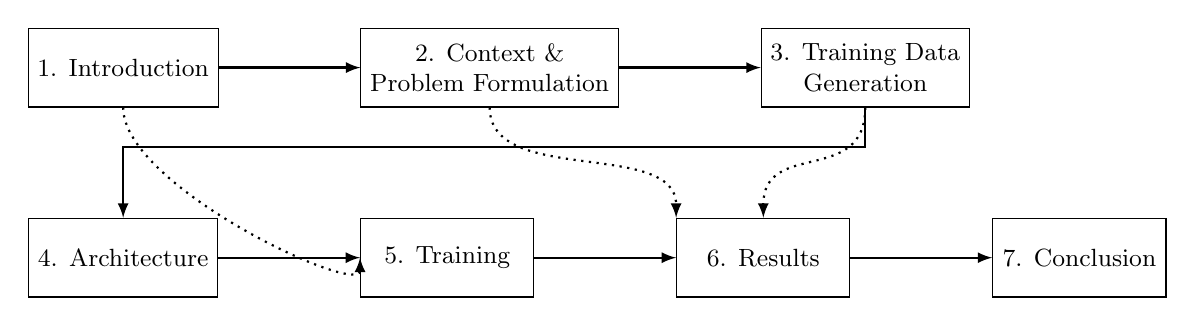
\begin{tikzpicture}[
    node distance=1.4cm and 1.8cm,
    every node/.style={draw, minimum width=2.2cm, minimum height=1.0cm, align=center, font=\small},
    solidarrow/.style={->, thick},
    dottedarrow/.style={->, thick, dotted}
]

% Top row
\node (intro) {1. Introduction};
\node (context) [right=of intro] {2. Context \& \\ Problem Formulation};
\node (data) [right=of context] {3. Training Data \\ Generation};

% Bottom row
\node (arch) [below=of intro] {4. Architecture};
\node (train) [right=of arch] {5. Training};
\node (results) [right=of train] {6. Results};
\node (concl) [right=of results] {7. Conclusion};

% Solid arrows
\draw[solidarrow] (intro) -- (context);
\draw[solidarrow] (context) -- (data);
\draw[solidarrow] (data.south) -- ++(0,-0.5) -| (arch.north);
\draw[solidarrow] (arch) -- (train);
\draw[solidarrow] (train) -- (results);
\draw[solidarrow] (results) -- (concl);

% Dotted cross-links (centered to Results)
\draw[dottedarrow] (intro.south) .. controls +(0,-1) and +(0,-0.5) .. (train.west);
\draw[dottedarrow] (context.south) .. controls +(0,-1.0) and +(0,1.0) .. (results.north west);
\draw[dottedarrow] (data.south) .. controls +(0,-1.0) and +(0,1.0) .. (results.north);

\end{tikzpicture}
\caption{Roadmap of this thesis. Solid arrows denote the main sequential flow of chapters. Dotted arrows indicate supporting or cross-referenced dependencies between chapters.}
\label{fig:thesis-roadmap}
\end{figure}

This section provided a high-level overview of our text. Chapter \ref{chap:problem-formulation} serves as an introduction to needed background, mainly in Causality and briefly to Deep Learning. It introduces Structural Causal Models (SCMs), their temporal extensions and known assumptions. Concerning Deep Learning, we provide a short overview on Deep Learning terminology for the uninitiated reader and elaborate on the Transformer architecture, which forms the backbone of our LCM, and on building blocks of neural nets that we utilize later on. In section \ref{sec:problem-formulation}, we formally define the main objective of our work. Chapter \ref{chap:data} details our synthetic data pipeline and the Temporal Causal Simulation (TCS) \& Adversarial Causal Tuning (ACT) frameworks for generating data pairs for training. Chapter \ref{chap:architecture} is dedicated to the architecture of our LCMs and input handling. Chapter \ref{chap:training} discusses training objectives, optimizers, and regularization methods that are essential for training of LCMs. Chapter \ref{chap:results} evaluates trained LCMs against baselines, with ablation and generalization studies. Chapter \ref{chap:conclusion} concludes the text with contributions, limitations, and future directions. We illustrate a roadmap of this thesis in Figure \ref{fig:thesis-roadmap}.
	%\chapter{Context \& Problem Formulation} \label{chap:problem-formulation}

\begin{chapquote}{\textit{Judea Pearl}}
``As X-rays are to the surgeon, graphs are for causation.''
\end{chapquote}

The main goal of this chapter is to underpin the essential theoretical background and terminology needed to formally define our work:  Causal discovery from time-series data using a foundational neural approach (our LCMs). The purpose of this part is to serve as a conceptual and notational bridge between the high-level motivation discussed in Chapter \ref{chap:introduction} and the following chapters. We focus on Temporal Structural Causal Models (TSCMs) and key assumptions needed for principled causal discovery. Rather than providing a complete treatment of the theory of Causality, our aim is to introduce the necessary formalism tailored to our own setting. For readers seeking a broader perspective on causality, we refer to the seminal works by \citet{pearl2009causality, pearl2018book}, \citet{spirtes2001causation} and \citet{peters2017elements}. For the case of causality and causal discovery in time-series, we point the reader to the works of \citet{runge2018causal, runge2023causal, assaad2022survey, gong2024causal}. We also elaborate on some important aspects of deep learning, as it also serves as an integral part of our work. For a reading on fundamentals, we suggest the textbook by \citet{goodfellow2016deep}. Section \ref{sec:scms} introduces Structural Causal Models, which are then extended to Temporal SCMs (TSCMs) in Section \ref{sec:temp-scms}, while Section \ref{sec:causal-assumptions} outlines the assumptions necessary for causal identifiability and model interpretation. Section \ref{sec:dl} provides a short overview of the necessary deep learning terminology for the unfamiliar reader. Finally, Section \ref{sec:problem-formulation} defines the main objective of our work.


\section{Structural Causal Models} \label{sec:scms}

The framework of Structural Causal Models is fundamental to Causality, as it represents the underlying causal mechanisms that govern an examined system. In order to start formally expressing \textit{\(X \text{ causes } Y\)}, one needs to define the observed variable \(Y\) as a function of \(X \). The notation \(:=\) is introduced to emphasize the asymetric nature of this relationship, rather than merely representing an algebraic equality. That is, \(X\) causes \(Y\), but not vice-versa. In the SCM framework, a variable \(Y\) is modeled as \(Y := f(X, \epsilon)\), where \(f\) is a deterministic (parametric or non-parametric) function, representing the causal mechanism and \(\epsilon\) an exogenous noiseterm which captures, among others, latent, unobserved factors and inherent randomness \citep{peters2017elements}. These noise variables are assumed to be mutually independent across variables and introduce the necessary stochasticity needed to model the causal mechanisms. Assuming no self-causation (a variable causing itself), the relationships between observed variables are qualitatively represented by a \textit{Directed Acyclic Graph (DAG)} where the direct causes of a variable \(X\) are the parents of \(Y\) in the DAG. As such, an edge \(X \rightarrow Y\) in the DAG encodes the causal information that \textit{\(X\) directly causes \(Y\)}. For example, consider the \textit{collider} structure \(X \rightarrow Z \leftarrow Y\), where \(X\) and \(Y\) share the same direct effect. This can be described by the equations \(Z := f(X, Y, \epsilon)\), \( X \sim \epsilon_X, ~Y \sim \epsilon_Y\) where \( \epsilon_X, \epsilon_Y\) are independent noise terms (e.g. sampled from a normal distribution) of \(X\) and \(Y\) respectively. An illustration is shown in Figure \ref{fig:scm}. If one ignores any causal interpretation of the functional mechanisms, this representation turns into a \textit{Structural Equation Model (SEM)}. Formally, we define an SCM as a tuple of (i) a set of \textit{endogenous} variables \(\mathcal{V}\), a set of \textit{exogenous} variables \(\mathcal{U}\) and the set \(\mathcal{F}\) of functions of the form \( f \equiv f(\text{Pa}(V_i),\epsilon_i)\), where \(\text{Pa}(V_i)\) denotes the direct causes of \(V_i\) (parents of \(V_i\) in the DAG), to generate each endogenous variable as a function of other variables. In practice, the functions \(f_i\) are often assumed to follow the form of an \textit{additive noise model (ANM)}. In this, case, the functional relationships are of the form 

\begin{equation}
    V_i := f(\text{Pa}(V_i), \epsilon_i) = f(\text{Pa}(V_i)) + \epsilon_i
\end{equation}

which simplifies estimation and data generation, while still allowing for representing a rich class of linear and non-linear causal mechanisms. In a nutshell, this serves as just another assumption to facilitate causal identifiability and inference.

\begin{figure}[t!]
\centering
\begin{minipage}{0.55\textwidth}
\centering
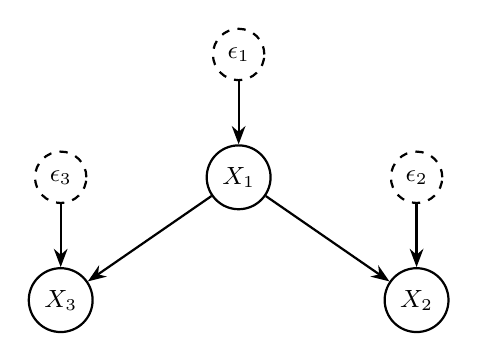
\begin{tikzpicture}[>=Stealth, node distance=1.2cm, every node/.style={circle, draw, minimum size=6mm, thick, font=\small}]		

% Nodes
\node (E1) [dashed] {$\epsilon_1$};
\node (X1) [below=of E1,yshift=0.4cm] {$X_1$};
\node (E2) [right=1.5cm of X1, dashed] {$\epsilon_2$};
\node (X2) [below=of E2,yshift=0.4cm] {$X_2$};
\node (E3) [left=1.5cm of X1, dashed] {$\epsilon_3$};
\node (X3) [below=of E3,yshift=0.4cm] {$X_3$};

% Edges
\draw[->, thick] (E1) -- (X1);
\draw[->, thick] (E2) -- (X2);
\draw[->, thick] (E3) -- (X3);
\draw[->, thick] (X1) -- (X2);
\draw[->, thick] (X1) -- (X3);

\end{tikzpicture}
\end{minipage}%
\hfill
\begin{minipage}{0.4\textwidth}
\centering
\vspace{1em}
\[
\begin{array}{l}
X_1 = f_1(\epsilon_1) \\[0.5em]
X_2 = f_2(X_1,\, \epsilon_2) \\[0.5em]
X_3 = f_3(X_1,\, \epsilon_3)
\end{array}
\]
\end{minipage}
\caption{Illustration of Structural Equation Model for an inverse collider structure \( X \leftarrow Z \rightarrow Y\). Each variable is a function of its direct causes and a noise term.} \label{fig:scm}
\end{figure}


\section{The Temporal Setup} \label{sec:temp-scms}

The case for time-series data can be seen an a natural generalization of the above, but taking into account the additional temporal dimension of data. Let \( \left\{ \mathbf{V}_t \right\}_{t \in \mathbb{Z}} \) denote a multivariate stochastic process, with \(V_t=(V^1_t,\ldots,V^N_t)\) representing the state of the system at time \(t\). A \textit{Temporal Structural Causal Model (TSCM)} consists of the structural assignments

\begin{equation} \label{eq:scm}
V^j_t \;:=\; f_j\bigl(\text{Pa}(V^j_t),\,\epsilon^j_t\bigr), ~\quad j=1,\dots,N,\;\;t\in\mathbb{Z},
\end{equation}

where for each variable index \(j\), \(\epsilon^j_t\) is an independent exogenous noise term, \( \text{Pa}(V^j_t)\;\subseteq\;\{V^i_{t-\tau}:i=1,2,\ldots,N,\;\tau=0,\ldots,,\ell_{\max}\}\setminus\{V^j_t\} \) denotes the \emph{causal parents} of \(V^j_t\) occurring at the same (if the existence of contemporaneous effects is assumed) or earlier time steps \(t-1,t-2,\ldots\), up to a finite maximal lag \(\ell_{\max}> 0\). Analogously to the atemporal case, each function \( f^j\) is the functional deterministic causal mechanism that determines the value of \(V^j_t\) given the direct causes \( \text{Pa}(V^j_t)\) and the corresponding noise term \(\epsilon^j_t\). The TSCM can then be written as a tuple \((\mathcal{G},\mathcal{F}, \mathcal{E})\) where \(\mathcal{G}\) is the causal graph, \(\mathcal{F}\) is the set of functional dependencies \(f^j\) and \(\mathcal{E}\) is the set of noise terms \(\epsilon^j_t\).  

The causal parents \(\text{Pa}(V^j_t)\), also called \textit{direct causes}, are selected from the set \(\{V^j_t, \ldots,  V^j_{t-\ell_\text{max}}\}\). This formalism encodes both lagged and contemporaneous causal effects (\(\ell_\text{max} = 0\)) to be represented, making it suitable for modeling a wide range of dynamical systems. To ensure well-posedness, we restrict all parent sets to occur at most \( \ell_\text{max} \) time-steps in the past, thus disallowing backward in-time causation. Recall that contemporaneous edges \(V^i_t \rightarrow V^j_t\) may occur if causal effects exist beyond the presumptive granularity (e.g. hourly causal mechanisms against a daily assumed lag). Furthermore, it is assumed that the temporal process is governed by a finite horizon of causal interactions and that each variable has a bounded number of causal inputs. Again, the functional relationships between the observed variables are represented by a DAG where edges move forward in time. As a concrete example, consider an observed process with the time-series \( V^1, V^2\) and \(V^3\) with the following causal relationships: Variable \(V^1\) directly causes variable \(V^2\) with lag \(1\) and \(V^2\) directly causes \(V^3\) with lag \(2\). As the process extends through time, so do the edges of the causal graph. The process (and as such the causal edges) may evolve, which makes the causal graph time-dependent. That is, different causal graphs may correspond to different time horizons and time windows. This pivots towards our first definition of the most important causal assumption for time-series data: \textit{Causal Stationarity}.

\begin{definition}[Causal Stationarity, \cite{runge2018causal}] Consider an SCM described as in Equation \ref{eq:scm}. If the causal relationships between variables \((V^i_{t-\tau}, V^j_t )\) for lag \(\tau>0\) also hold for all time-shifted versions \((V^i_{t' -\tau}, V^j_{t'}) \), the described process is \textit{causally stationary}. Informally, the graph structure and noise distribution of the SCM are time-invariant.
\end{definition}

Using the previous example, that means that, for the current timepoint \(t\), there exist causal edges such as \( V^1_{t-1} \rightarrow V^2_t \) and \( V^2_{t-2} \rightarrow V^3_t \). By causal stationarity, these relations also hold for their time-shifted versions: \( V^1_{t'-1} \rightarrow V^2_{t'} \) and \( V^2_{t'-2} \rightarrow V^3_{t'} \) for all \( t' \leq t \). Like in the atemporal case, indirect causation is implied through directed paths. In literature, this invariance of causal effects in time is also referred to as time homogeneity \citep{gong2024causal}.

The causal dependencies implied by a TSCM can be visualized as a directed graph unrolled over time. The cautious reader may have observed that due to the temporal axis, multiple graph abstractions are possible depending on the intended level of granularity. We first define the most complete representation, the \textit{full-time causal graph}:

% Full Time Causal Graph (a)
\begin{figure}[t!]
\centering
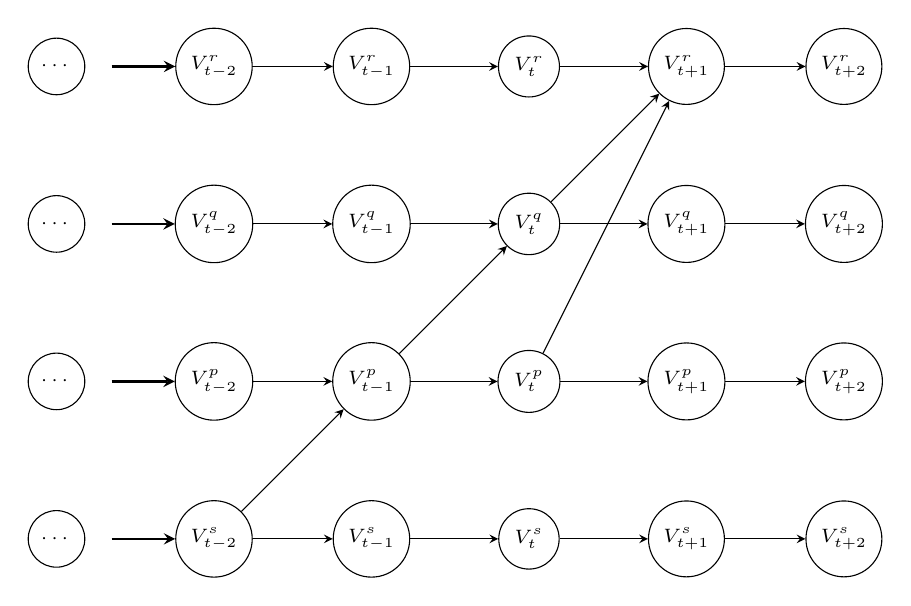
\begin{tikzpicture}[
    every node/.style={circle, draw, minimum size=0.5cm, font=\scriptsize},
    >=stealth,
    ->,
]

% Coordinates and ellipsis
\foreach \i/\y in {r/6, q/4, p/2, s/0} {
    % Main nodes from t-2 to t+2
    \foreach \j/\x in {-2/-4, -1/-2, 0/0, 1/2, 2/4} {
        \node (\i\j) at (\x,\y) {$V^{\i}_{t\ifnum\j<0 \j\else\ifnum\j=0 \else+\j\fi\fi}$};
    }
    % Dots on the far left
    \node at (-6,\y) {$\cdots$};
    % Arrows from dots to first node
    \draw[->, thick] (-5.3,\y) -- (\i-2);
}

% Temporal self-links
\foreach \i in {r,q,p,s} {
    \foreach \j/\k in {-2/-1, -1/0, 0/1, 1/2} {
        \draw (\i\j) -- (\i\k);
    }
}

% Cross-temporal causal edges
\draw (s-2) -- (p-1);
\draw (p-1) -- (q0);
\draw (q0) -- (r1);
\draw (p0) -- (r1);

\end{tikzpicture}
\caption{Full time causal graph: The temporal SCM extends infinitely into the past (indicated by \(\cdots\) and incoming arrows) and shows both auto- and cross-variable lagged dependencies. Notice that in this example, no causal stationarity is assumed.}
\label{fig:full-time-causal-graph}
\end{figure}

\begin{definition}[Full-Time Causal Graph]
Let \(\left\{ \mathbf{V}_t \right\}_{t \in \mathbb{Z}}\) be a multivariate stochastic process governed by a Temporal SCM. The \textit{full-time causal graph} is the infinite directed acyclic graph (DAG) whose nodes are all variables \(V^i_t\) for every \(i \in \{1, \dots, N\}\) and every time step \(t \in \mathbb{Z}\), and whose edges correspond to direct causal relationships \(V^i_{t - \tau} \rightarrow V^j_t\) as defined by the TSCM. This graph includes both within-variable (autoregressive) and cross-variable temporal dependencies across all lags up to \(\ell_{\max}\).
\end{definition}

Figure \ref{fig:full-time-causal-graph} illustrates such a structure, where both temporal self-dependencies and cross-variable influences are made explicit. This infinite graph represents the most faithful unfolding of the SCM in time. If causal stationarity is not assumed (as illustrated), then different causal graphs correspond to different time horizons, further complicating the causal discovery task. Secondly, the full-time causal graph can be truncated to a specific time-horizon, resulting in the \textit{time-lagged (also called \textit{windowed}) causal graph}, with causal edges up to \(\ell_\text{max}\). 

\begin{definition}[Lagged Causal Graph - Window Causal Graph]
A \textit{lagged causal graph} is a directed acyclic graph (DAG) that represents causal relationships between time-shifted variables in a multivariate time-series. Formally, let \(\mathbf{V}_t = \{V^1_t, V^2_t, \dots, V^k_t\}\) denote the set of observed variables at time step \(t\). A lagged causal graph \(\mathcal{G}\) contains directed edges of the form \(V^i_{t-\tau} \rightarrow V^j_t\), where \(\tau \in \{1, 2, \dots, \ell_{\max}\}\) is a positive time lag. An edge \(V^i_{t-\tau} \rightarrow V^j_t\) indicates that \(V^i\) is a direct cause of \(V^j\) with a time lag of \(\tau\).
\end{definition}

An example of a lagged causal graph is illustrated in Figure \ref{fig:temporal-graphs} (a). Finally, the lagged causal graph can be further simplified to a more concise representation, the \textit{summary causal graph}.

\begin{definition}[Summary Causal Graph]
 Given a lagged causal graph \(\mathcal{G}\) with edges of the form \(V^i_{t-\tau} \rightarrow V^j_t\) for various lags \(\tau\), the corresponding summary graph \(\mathcal{S}\) contains an edge \(V^i \rightarrow V^j\) if there exists at least one lag \(\tau\) such that \(V^i_{t-\tau}\) is a direct cause of \(V^j_t\) in \(\mathcal{G}\).
\end{definition}

Essentially, a summary graph is a simplified representation of the lagged causal structure in a time-series, where the temporal information about lags is abstracted away, as shown in Figure \ref{fig:temporal-graphs} (b). The summary graph collapses temporal information and only displays whether a causal relationship exists between two variables, but it does not specify the lag or delay at which the causal influence occurs. Note that from a lagged causal graph one can obtain the summary graph (e.g. from Figure \ref{fig:temporal-graphs} (a) to Figure \ref{fig:temporal-graphs} (b)), but not vice-versa, as the lag of causal relationships is not encoded in the summary structure. Summary graphs that retain temporal information can of course be obtained from the lagged causal graph, but remain outside the scope of our text.   

\begin{figure}[t!]
\centering

% Lagged and Summary Graph Side-by-Side
\begin{minipage}[t]{0.48\textwidth}
\centering
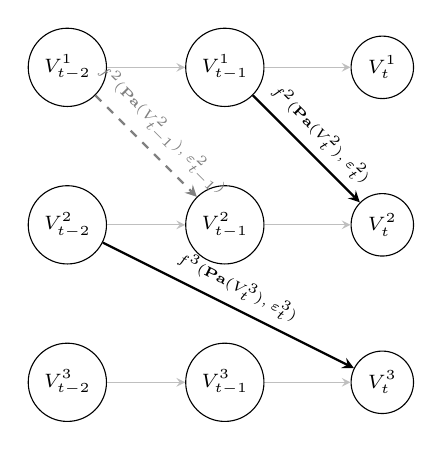
\begin{tikzpicture}[
    varnode/.style={circle, draw, minimum size=0.6cm, font=\scriptsize},
    >=stealth,
    ->,
    dashededge/.style={->, dashed, thick, color=gray},
    solidedge/.style={->, thick},
]

% t-2
\node[varnode] (V1t2) at (0,4) {$V^1_{t-2}$};
\node[varnode] (V2t2) at (0,2) {$V^2_{t-2}$};
\node[varnode] (V3t2) at (0,0) {$V^3_{t-2}$};

% t-1
\node[varnode] (V1t1) at (2,4) {$V^1_{t-1}$};
\node[varnode] (V2t1) at (2,2) {$V^2_{t-1}$};
\node[varnode] (V3t1) at (2,0) {$V^3_{t-1}$};

% t
\node[varnode] (V1t) at (4,4) {$V^1_{t}$};
\node[varnode] (V2t) at (4,2) {$V^2_{t}$};
\node[varnode] (V3t) at (4,0) {$V^3_{t}$};

% Optional: temporal arrows (light gray)
\foreach \i in {1,2,3} {
  \draw[->, gray!50] (V\i t2) -- (V\i t1);
  \draw[->, gray!50] (V\i t1) -- (V\i t);
}

% Causal arrows with functional labels directly on edges
\draw[solidedge] (V1t1) -- (V2t)
  node[midway, above, sloped, font=\tiny, draw=none, fill=none] 
  {$f^{2}(\mathbf{Pa}(V^2_t),\varepsilon^2_t)$};

\draw[dashededge] (V1t2) -- (V2t1)
  node[midway, above, sloped, font=\tiny, draw=none, fill=none] 
  {$f^{2}(\mathbf{Pa}(V^2_{t-1}),\varepsilon^2_{t-1})$};

\draw[solidedge] (V2t2) -- (V3t)
  node[midway, above, sloped, font=\tiny, draw=none, fill=none] 
  {$f^{3}(\mathbf{Pa}(V^3_t),\varepsilon^3_t)$};

\end{tikzpicture}


\vspace{0.5em}
{(a) Lagged causal graph}
\end{minipage}
\hfill
\begin{minipage}[t]{0.48\textwidth}
\centering
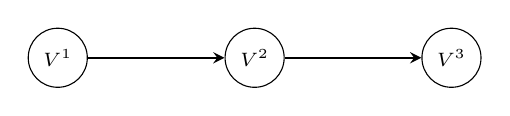
\begin{tikzpicture}[
    every node/.style={circle, draw, minimum size=0.6cm, font=\scriptsize},
    >=stealth,
    ->,
]

\node (V1) at (2,2) {$V^1$};
\node (V2) at (4.5,2) {$V^2$};
\node (V3) at (7,2) {$V^3$};

\draw[->, thick] (V1) -- (V2);
\draw[->, thick] (V2) -- (V3);

\end{tikzpicture}

\vspace{0.5em}
{(b) Summary causal graph}
\end{minipage}

\caption{Illustration of a temporal SCM with max lag \(\ell_{\max}=2\). (a) The lagged causal graph shows variable \(V^1\) causing \(V^2\) with lag 1 and \(V^2\) causing \(V^3\) with lag 2. Dashed edges encode the assumption of causal stationarity, meaning that the same causal dependencies recur over time. Functional dependencies between lagged variables are shown directly on the edges. (b) The summary causal graph discards time lag information, representing only the aggregated causal influences.}
\label{fig:temporal-graphs}
\end{figure}

\section{Probabilistic Quantifications} \label{sec:bns}

To introduce our next causal assumptions, one needs to understand how causal structures relate to probabilistic reasoning, by the formalism of \textit{Bayesian networks (BNs)}. BNs provide a compact representation of a joint probability distribution using a directed acyclic graph. Each node corresponds to a random variable, and each directed edge represents a statistical dependence.

Briefly, a Bayesian network is defined as a pair \((\mathcal{G}, \mathbb{P})\), where \(\mathcal{G} = (\mathbf{V}, \mathcal{E})\) is a DAG with nodes \(\mathbf{V} = \{X_1, \dots, X_n\}\), and \(\mathbb{P}\) is a joint distribution over \(\mathbf{V}\), which factorizes, according to the chain rule, based on the structure of \(\mathcal{G}\). That is, each variable \(X_i\) is conditionally independent of its non-descendants given its parents \(\mathrm{Pa}(X_i)\) in the graph:

\begin{equation}
\mathbb{P}(X_1, \dots, X_n) = \prod_{i=1}^n \mathbb{P}(X_i \mid \mathrm{Pa}(X_i)).
\end{equation}

This factorization, which \citet{bengio2019meta} call \textit{disentangled factorization}, provides both computational efficiency and semantic clarity: each conditional distribution models a local dependency, and the global distribution emerges from their composition. Compared to SCMs which explicitly model causal mechanisms through assignments \(X_i := f_i(\mathrm{Pa}(X_i), \epsilon_i)\), BNs represent probabilistic dependencies only. While every SCM induces a Bayesian Network (through the distribution entailed by its noise and mechanisms), the converse does not hold; Bayesian Networks may not capture the directionality or manipulability implied by causality, so interventions and counterfactuals are not applicable. If one assumes causal interpretation on the edges, the resulting BN can be treated as a \emph{causal BN}. In a nutshell, the key advantage of Bayesian Networks lies in their ability to encode and reason about conditional independencies, which are central to many causal discovery approaches.


\section{Causal Assumptions} \label{sec:causal-assumptions}

We now elaborate on causal assumptions needed for performing identifiability of the true causal graph and consequently, sound causal inference. We have already elaborated on the assumption of causal stationarity in Section \ref{sec:temp-scms}. All causal discovery algorithms are governed by a set of assumptions, regarding the statistical properties of the data and the underlined structure of the causal model. Is is thus evident that making and understanding causal assumptions is also vital for correct interpretation not only of the discovered causal structure. We define the following assumptions in a way to be applied to either a (standard) causal graph or analogously to a temporal causal graph.

\begin{definition}[Causal Markov Condition, \citep{spirtes2001causation}] Let \(\mathcal{G}\) be a causal graph with vertex set \(\mathbf{V}\) and \(\mathbb{P}\) a probability distribution over \(\mathbf{V}\), generated by the causal structure induced by \(\mathcal{G}\). Then \(\mathcal{G}\) and \(\mathbb{P}\) satisfy the Markov Condition if and only if \(~\forall ~W \in \mathbf{V}\), \(W\) is independent of its non-descendants (non causal effects) given its parents (direct causes) on \(\mathcal{G}\).
\end{definition}

Essentially, the Causal Markov Condition assures that conditional independences between variables are exactly those entailed by the causal graph (i.e. by d-separation).

\begin{definition}[Faithfulness, \citep{spirtes2001causation}] Let \(\mathcal{G}\) be a causal graph and \(\mathbb{P}\) a probability distribution over \(\mathbf{V}\). We say that \(\mathcal{G}\) and \(\mathbb{P}\) are faithful to each other if and only if (iff) the all and only the independence relations of \(\mathbb{P}\) are entailed by the Causal Markov condition of \(\mathcal{G}\). Specifically, \(\mathcal{G}\) and \(\mathbb{P}\) satisfy the Faithfulness Condition if-f every conditional independence relation true in \(\mathbb{P}\) is entailed by the Causal Markov Condition applied to \(\mathcal{G}\).
\end{definition}

In other words, given a causally sufficient set of variables \(\mathcal{U}\) in a population \(N\), \textit{every} conditional independence relation that holds in the density over \(\mathcal{U}\) \textit{is entailed by the local directed Markov condition for the causal DAG of \(N\)}. The key argument behind assuming faithfulness of the true causal graph and the corresponding distribution induced by observed data is that non-faithfulness would lead to determinism in the observed system. As everything would cause everything and no stochasticity is involved, performing causal queries would prove invalid.  

\begin{definition}[Causal Sufficiency, \citep{spirtes2001causation}] A set \(\mathbf{V}\) of variables is causally sufficient for a population iff in the population every common cause of any two or more variables in \(\mathbf{V}\) is in \(V\), or has the same value for all units in the population. The common cause \(Z\) of two or more variables in a DAG \(X \leftarrow Z \rightarrow Y\) is called a \textit{confounder of \(X\) and \(Y\)}. Hence causal sufficiency implies no unobserved confounders. The notion of causal sufficiency is being used without explicitly mentioning the population.
\end{definition}

\begin{figure}[ht!]
\begin{multicols}{2}
	\begin{center}
		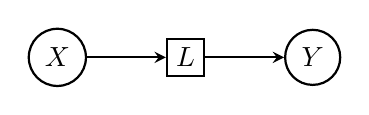
\begin{tikzpicture}[->,>=stealth,thick]
			% X -> L -> Y
			\node[draw, circle] (XLY1) {$X$};
			\node[draw, rectangle,right=of XLY1] (L1) {$L$};
			\node[draw, circle,right=of L1] (Y1) {$Y$};
			
			\draw[->] (XLY1) -- (L1);
			\draw[->] (L1) -- (Y1);
		\end{tikzpicture}
	\columnbreak

		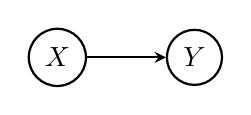
\begin{tikzpicture}[->,>=stealth,thick]
			% X <-> Y
			\node[draw, circle] (XY1) {$X$};
			\node[draw, circle,right=of XY1] (Y1) {$Y$};
			
			\draw[->] (XY1) -- (Y1);
		\end{tikzpicture}
	\end{center}
\end{multicols}

\begin{multicols}{2}
	\begin{center}
		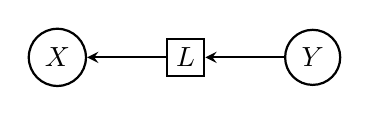
\begin{tikzpicture}[->,>=stealth,thick]
			% X <-> L <-> Y
			\node[draw, circle] (XLY2) {$X$};
			\node[draw, rectangle,right=of XLY2] (L2) {$L$};
			\node[draw, circle,right=of L2] (Y2) {$Y$};
			
			\draw[<-] (XLY2) -- (L2);
			\draw[<-] (L2) -- (Y2);
		\end{tikzpicture}
	
	    \columnbreak
	    
		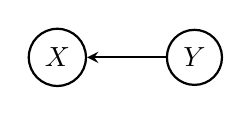
\begin{tikzpicture}[->,>=stealth,thick]
			% X <-> Y
			\node[draw, circle] (XY2) {$X$};
			\node[draw, circle,right=of XY2] (Y3) {$Y$};
			
			\draw[<-] (XY2) -- (Y3);
		\end{tikzpicture}
	\end{center}
\end{multicols}

\begin{multicols}{2}
		\begin{center}
		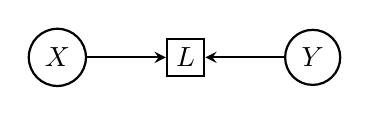
\begin{tikzpicture}[->,>=stealth,thick]
			% X <-> L <-> Y
			\node[draw, circle] (XLY2) {$X$};
			\node[draw, rectangle,right=of XLY2] (L2) {$L$};
			\node[draw, circle,right=of L2] (Y2) {$Y$};
			
			\draw[->] (XLY2) -- (L2);
			\draw[<-] (L2) -- (Y2);
		\end{tikzpicture}
	\end{center}
    \columnbreak
	\begin{center}
		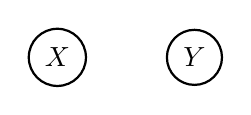
\begin{tikzpicture}[->,>=stealth,thick]
			% X <-> Y
			\node[draw, circle] (XY2) {$X$};
			\node[draw, circle,right=of XY2] (Y3) {$Y$};
			
		\end{tikzpicture}
	\end{center}
\end{multicols}

\begin{multicols}{2}
	\begin{center}
		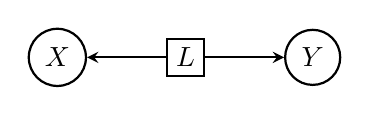
\begin{tikzpicture}[->,>=stealth,thick]
			% X <-> L <-> Y
			\node[draw, circle] (XLY2) {$X$};
			\node[draw, rectangle,right=of XLY2] (L2) {$L$};
			\node[draw, circle,right=of L2] (Y2) {$Y$};
			
			\draw[<-] (XLY2) -- (L2);
			\draw[->] (L2) -- (Y2);
		\end{tikzpicture}
	\end{center}
	
	\columnbreak
	
	\begin{center}
		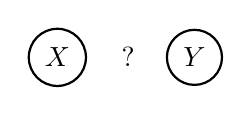
\begin{tikzpicture}[->,>=stealth,thick]
			\node[draw, circle] (XY2) {$X$};
			\node[draw, circle,right=of XY2] (Y3) {$Y$};
			\node at (0.9,0) {?};
		\end{tikzpicture}
	\end{center}
\end{multicols}
\caption{Illustrations for the presence of a hidden confounder \(L\) for two variables \(X,Y\), in the case of atemporal data. In the first case, where \(X\) indirectly causes \(Y\) with \(L\) acting as a mediator, we observe that \(Dep(X,Y)\) so we infer \(X \rightarrow Y\), and similarly \(X \leftarrow Y\) in the second case. In the third case where \(X\) and \(Y\) share a hidden common effect, we infer \(Indep(X,Y)\) and thus discover no edge between \(X\) and \(Y\). However, in the case of \(L\) being a hidden common cause of \(X\) and \(Y\), there exists no DAG that captures the dependencies.}
\label{fig:dag-conf}
\end{figure}

To put it simply, causal sufficiency is the \textit{asumption of no unobserved variables}. Unobserved variables are called \textit{latent} or \textit{hidden}. The fact that DAGs are unable to adequately capture latent confounders becomes apparent in the example at Figure \ref{fig:dag-conf}, for the case of i.i.d. data. The assumption can be adapted similarly for the case of time-series, where one can assume latent confounders may exist at a predefined time-lag. For example \(V^1_{t}\) and \(V^2_{t}\) may be confounded by the latent variable \(V^3_{t-1}\). SCMs without unobserved confounders are also called \textit{Markovian models} as the noise terms of the variables are independent. The observed variables in SCMs with unobserved confounding can have dependent noise terms, called \textit{semi-Markovian models}.

It must be noted that in practice, not all variables in the underlying SCM are measured. A projected causal graph on the observed subset is represented as an \textit{Acyclic Directed Mixed Graph} (ADMG), in which a bidirected arrow \(V^i_{t-\tau}\leftrightarrow V^j_t\) indicates the presence of an unobserved common cause with lag \(\tau\). For atemporal data, causal structures that enable marginalization of an SCM (a model with a subset of variables) exist \citep{richardson2002ancestral}, but remain completely outside our scope. This formulation also underlies algorithms for causal discovery under latent confounding, or when inferring contemporaneous effects where directionality is unknown.

\begin{figure}[h]
\centering
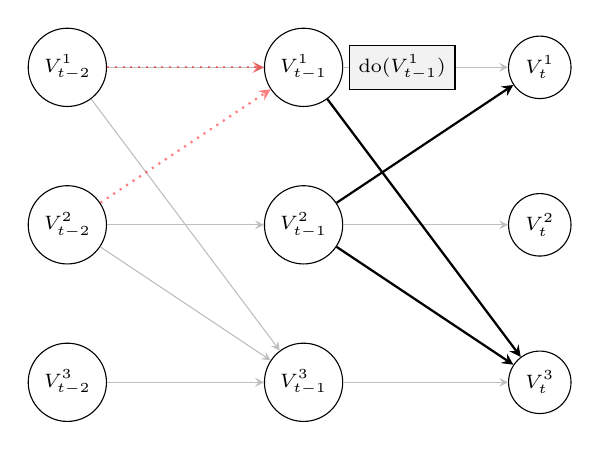
\begin{tikzpicture}[
    every node/.style={circle, draw, minimum size=0.6cm, font=\scriptsize},
    >=stealth,
    ->,
    solidedge/.style={->, thick},
    removededge/.style={->, red, dotted, thick, opacity=0.5},
    interbox/.style={rectangle, draw, minimum width=0.5cm, minimum height=0.4cm, font=\tiny, fill=black!5}
]

% Nodes at t-2
\node (V1t2) at (0,6) {$V^1_{t-2}$};
\node (V2t2) at (0,4) {$V^2_{t-2}$};
\node (V3t2) at (0,2) {$V^3_{t-2}$};

% Nodes at t-1
\node (V1t1) at (3,6) {$V^1_{t-1}$};
\node (V2t1) at (3,4) {$V^2_{t-1}$};
\node (V3t1) at (3,2) {$V^3_{t-1}$};

% Nodes at t
\node (V1t) at (6,6) {$V^1_{t}$};
\node (V2t) at (6,4) {$V^2_{t}$};
\node (V3t) at (6,2) {$V^3_{t}$};

% Temporal identity edges (gray)
\foreach \i in {1,2,3} {
  \draw[->, gray!50] (V\i t2) -- (V\i t1);
  \draw[->, gray!50] (V\i t1) -- (V\i t);
}

% Causal edges
\draw[->, gray!50] (V1t2) -- (V3t1);     % V^1_{t-2} -> V^3_{t-1}
\draw[solidedge] (V1t1) -- (V3t);        % V^1_{t-1} -> V^3_t
\draw[->, gray!50] (V2t2) -- (V3t1);     % V^2_{t-2} -> V^3_{t-1}
\draw[solidedge] (V2t1) -- (V1t);        % V^2_{t-1} -> V^1_t
\draw[solidedge] (V2t1) -- (V3t);        % V^2_{t-1} -> V^3_t

% Removed incoming edges to V1_{t-1}
\draw[removededge] (V1t2) -- (V1t1);     % V^1_{t-2} -> V^1_{t-1} (self-dependence, optional)
\draw[removededge] (V2t2) -- (V1t1);     % V^2_{t-2} -> V^1_{t-1}

% Intervention label
\node[interbox, right=2pt of V1t1] {\scriptsize do($V^1_{t-1}$)};

\end{tikzpicture}
\caption{A dense lagged causal graph with an intervention on \( V^1_{t-1} \), where \(V^2\) directly causes \(V^1\) \& \(V^3\) with lag 1 and \(V^1\) directly causes \(V^3\) with lag 1. The intervention \( \text{do}(V^1_{t-1}) \) removes all incoming edges to \( V^1_{t-1} \), shown as red dotted lines, while preserving its downstream influence on \( V^3_t \). The interventional value replaces the natural dynamics of \( V^1_{t-1} \), breaking any backdoor paths through its original causes.
}
\label{fig:interv-example}
\end{figure}

As we have seen in Chapter \ref{chap:introduction}, the first rung that differentiates a probabilistic model with a causal model is the ability to perform interventions, that is, modifying the internal causal mechanisms of the examined system. We define interventions for the temporal setting, which only differs in the temporal dimension of the variables. TSCMs allow interventions to be performed in a simple manner: Modify the structural assignment in the SCM of a variable \(X^k\) to \(x\). This corresponds to a \textit{hard intervention} at a specific timestep \(t\). The resulting interventional distribution \(\mathbb{P}(Y_t|\text{do}(X^k_t=x))\) captures the causal effect of setting \(X\) to \(x\). The reader should recall that the observational and interventional distributions may differ because non-causal associations (e.g., due to confounders) are blocked under interventions. In the causal graph, this corresponds to performing \textit{graph surgery}, by removing all incoming edges to \(X^k_t\) and replacinb the structural equation with \(X^k_t:=x\), due to what is known as the \textit{modularity assumption}. An example is illustrated in Figure \ref{fig:interv-example}. One may also apply different interventions to different variables \(X^i_t, X^j_t\), (\textit{multiple interventional targets}) at the same timestep, resulting in an interventional distribution \( \mathbb{P}(Y_t | \text{do}(X^i_t=x^i_t, X^j_t=x^j_t))\). For soft interventions, as the name may suggest, instead of explicitely modifying the structural assignment, one adds a noise term (either sampled from a known parametric distribution like a Gaussian, or sampled from a prior distribution) to the structural assignment. Consequently, interventions allow us to define causality in a much more rigid manner: A variable \(X^i\) causes \(X^j\) if an intervention on \(X^i\) leads to a direct change in \(X^j\). Conclusively, do-calculus provides a set of transformation rules to express interventional (and counterfactual, although outside of our scope) distributions in terms of observable quantities, given a true or discovered causal graph. It underpins identification results, determining whether a causal effect can in principle be recovered from observational data alone or whether additional assumptions or interventional data are required. For causal discovery algorithms, handling of interventional data leads further into correct identifiability of the true causal graph, which may not be possible with observational data alone. 

\section{Brief Deep Learning Overview} \label{sec:dl}

This section aims to provide a high-level overview of deep learning for the unfamiliar reader, which is the second important pillar our work is based on. 

The backbone of deep learning is the concept of \textit{artificial neural network (ANN)}, abbreviated as neural network (NN). Such a network consists of a collection of connected units named neurons. The name stems from the introduction of the first model, Rosenblatt's Multilayer Perceptron (MLP) \citep{rosenblatt1958perceptron}, which loosely mimics the connection of biological neurons in the brain. Each neuron is connected to other neurons like a synapse in the brain, with signal being propagated throught the network using weights associated with the connections, which are real numbers. The larger the number, the stronger the connection.

\begin{figure}[h]
    \centering
    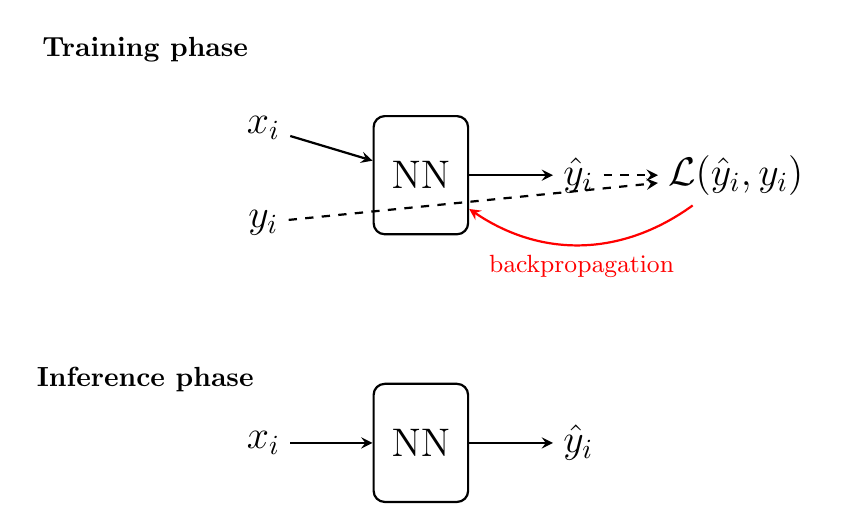
\begin{tikzpicture}[>=stealth, thick, node distance=1.8cm]
        % Training phase
        \node at (-1.5, 2) {\textbf{Training phase}};
        \node (xtrain) at (0,1) {\Large $x_i$};
        \node (ytrain) at (0,-0.2) {\Large $y_i$};
        \node[draw, rounded corners, minimum width=1.2cm, minimum height=1.5cm] (nntrain) at (2,0.4) {\Large NN};
        \node (yhattrain) at (4,0.4) {\Large $\hat{y}_i$};
        \node (loss) at (6,0.4) {\Large $\mathcal{L}(\hat{y}_i, y_i)$};

        % Training arrows
        \draw[->] (xtrain) -- (nntrain);
        \draw[->] (nntrain) -- (yhattrain);
        \draw[->, dashed] (ytrain) -- (loss);
        \draw[->, dashed] (yhattrain) -- (loss);
        \draw[->, thick, red] (loss) to[bend left=35] node[midway, below] {\small backpropagation} (nntrain);
        % Inference phase
        \node at (-1.5, -2.2) {\textbf{Inference phase}};
        \node (xtest) at (0,-3) {\Large $x_i$};
        \node[draw, rounded corners, minimum width=1.2cm, minimum height=1.5cm] (nntest) at (2,-3) {\Large NN};
        \node (yhattest) at (4,-3) {\Large $\hat{y}_i$};
        % Inference arrow
        \draw[->] (xtest) -- (nntest);
        \draw[->] (nntest) -- (yhattest);

    \end{tikzpicture}
    \caption{Illustration of neural network training and inference. During training, both input-output pairs \((x_i, y_i)\) are provided to compute the loss \(\mathcal{L}(\hat{y}_i, y_i)\) and update model parameters via backpropagation. During inference, only the input \(x_i\) is given, and the trained network produces an estimated output \(\hat{y}_i\).}
    \label{fig:nn-train-infer}
\end{figure}

Similarly to supervised learning algorithms, a neural network assumes a data input and constructs an output, based on a collection of data instances, in order to find a suitable representation between them, via a process called \textit{training}. By processing such ground truth input and output pairs, training the model employs a \textit{supervised learning scheme} (see Figure \ref{fig:nn-train-infer}). In practice, training the model refers to adjusting its set of trainable parameters (such as the weight between neurons as illustrated before) in order to find the relationship between the input and target data pairs (assuming it exists). Training such a model consists of numerous important steps. As training consists of a mathematical optimization approach (since the problem is intractable), the goal is to minimize an objective function (loss function) that measures the error in performance, often as the absolute difference between the model's estimated outputs and the ground truth targets. Minimization of such a function is attained by the adjustment of the trainable parameters, which occurs iteratively as dictated by the training \textit{optimizer}, based on gradients computed through \textit{backpropagation} \citep{lecun1988theoretical, werbos2002backpropagation}. Backpropagation applies the chain rule of calculus in reverse (illustrated in Figure \ref{fig:building-blocks}), computing how much each parameter contributed to the error signal. This allows the optimizer to make informed adjustments. Common optimizers include Stochastic Gradient Descent (SGD) \citep{ruder2016overview} and Adam \citep{kingma2015adam}, both of which aim to efficiently navigate the high-dimensional loss landscape.

Once trained, the model can generalize to unseen data in the \textit{inference phase}, where it takes only input \(x_i\) and outputs a prediction \(\hat{y}_i\). Neural network models are known as universal approximators \citep{hornik1989multilayer}. This illustrates that in cases where statistical, machine learning, or even very simple methods fail due to the intractable nature of the function \(f\) between input and output, it becomes significant to consider fitting a neural network model.

Progress in neural networks and deep learning has often been driven by the development of general-purpose architectures that outperform prior methods across a wide range of tasks. Some advancements stem from novel ideas that reshape the field, while others result from the resurgence of older techniques enabled by increased data availability and computational power. Early models such as perceptrons \citep{rosenblatt1958perceptron} laid the foundation for modern neural networks, but their inability to represent non-linearly separable functions, such as XOR \citep{minsky1969perceptrons}, led to skepticism and a temporary stagnation in research. During the 1980s and 1990s, more expressive models were proposed, including self-organizing maps (SOMs) \citep{kohonen1982self}, Hopfield networks \citep{hopfield1982neural} and Boltzmann machines \citep{ackley1985learning}, all of which introduced new paradigms in unsupervised learning, associative memory and energy-based modeling. With the resurgence of deep learning, driven by larger datasets and modern hardware, architectures like feedforward networks, convolutional neural networks (CNNs) \citep{lecun1989backpropagation}, recurrent neural networks (RNNs) \citep{rumelhart1986learning} and LSTMs \citep{hochreiter1997long} became dominant in practical applications. Meanwhile, methods such as support vector machines (SVMs) \citep{cortes1995support} and conditional random fields (CRFs) \citep{lafferty2001conditional} contributed significantly to structured prediction tasks before deep learning approaches took center stage. A key turning point came with the introduction of Transformers \citep{vaswani2017attention}, which moved beyond the limitations of recurrence-based models by relying entirely on attention mechanisms. This shift enabled greater parallelism and improved the ability to capture long-range dependencies, particularly in sequential and structured data. Transformers have since become the backbone of modern foundation models, which aim to generalize across diverse tasks by leveraging vast amounts of data, compute, and expressive representations, an idea that also underpins the work proposed in this thesis.

A neural network consists of multiple \textit{layers}, which may be of the same kind or of different kind, the combination of which can be selected in almost any desired order. A \textit{sequential} architecture consists of layers that are linearly stacked, that is, each layer receives input from only its previous layers and only outputs to its forward layers. The first layer is usually referred to as the \textit{input} layer and the last one as the \textit{output} layer, with the in-between layers referred as \textit{hidden layers} (unscreen blocks). In a way, such a neural architecture can be thought as a stack of building blocks, each of which is responsible for a specific task, from bottom to top (Figure \ref{fig:building-blocks}). All layers consist of different number of parameters (real numbers, vectors or matrices) based on their design. The parameters that are tunable during training are called \textit{trainable} or \textit{learnable parameters}. The collection \(\theta\) of trainable parameters represent the neural network \(f_\theta\). Typically those are the weights (noted by \(W\), \(w\), or \(U\), \(u\)) and biases (notated \(b\)). Depending on the layer's defined operation, these weights are applied to its input \(x\), and by adding the biases \(b\), one obtains its resulting output \(y\). This output will then be fed as input into the next layer and so forth, until the output layer delivers the final estimation of the model. Layers that do not introduce any trainable parameters exist, such as ones that apply operations (e.g. averaging, pooling etc.). They are usually added in order to prepare the data from the previous layer to be fed to the upcoming layers. They may also be applied by taking the network's final output layer and formulating the final predictions of the overall model.

\begin{figure}[ht!]
    \centering
    \begin{tikzpicture}
        % Draw the module
        \draw[thick] (-2, 1) rectangle (2, -1);
        \node at (0, 0) {$f$};
        
        % Input x
        \draw[->, thick, green!50!black] (-3, 0) -- (-2, 0);
        \node[above, green!50!black] at (-2.5, 0) {$x$};
        
        % Output y
        \draw[->, thick, green!50!black] (2, 0) -- (4, 0);
        \node[above, green!50!black] at (2.5, 0) {$y$};
        
        % Gradients
        \draw[<-, thick, red] (-3, -0.5) -- (-2, -0.5);
        \node[below, red] at (-2.5, -0.5) {$\frac{\partial E}{\partial x}$};
        
        \draw[<-, thick, red] (3, -0.5) -- (2, -0.5);
        \node[below, red] at (2.5, -0.5) {$\frac{\partial E}{\partial y}$};
        
        \node[red] at (0, -0.8) {$\frac{\partial y}{\partial x}$};
        
        % Chain rule
        \node[red] at (-2.5, -1.5) {$\frac{\partial E}{\partial x} = \frac{\partial E}{\partial y} \cdot \frac{\partial y}{\partial x}$};

        % Lego placeholder
        \node at (7, 0) {\includegraphics[width=5cm]{images/building_blocks.jpg}};
    \end{tikzpicture}
    \caption{Training deep neural networks can be thought as building blocks, leaving architecture and capabilities to the imagination, with gradients being computed during backpropagation.} \label{fig:building-blocks}
\end{figure}

Apart from selecting the architecture of the model, consisting of the type, amount and order of layers, there are other types of parameters to choose from within each specific layer. Such are called \textit{hyperparameters} such as weight initializers, stride, dilation rate, padding etc. In order to successfully train a network, optimal selection of layers, parameters and hyperparameters, as well as their initialization, are all crucially important. Overall, assembling a neural network model after defining the problem at hand is a non-trivial and demanding task. It requires familiarity with the specific problem, creativity, competence and knowledge within the area of neural networks, plus being informed about the latest advancements and state-of-the-art approaches. It should be noted that selection of the ideal architecture and parameters is a different field at first place, as inevitably to this day it still requires careful fiddling, guessing, experimental trial-and-error proceduces and at many times ad-hoc approaches that are empirically shown to improve the state-of-the-art. Finally, although simple in theory, training deep models in practice presents challenges such as vanishing gradients, overfitting, and instability. Techniques like normalization layers, residual connections, and regularization help mitigate these issues. A discussion on how some of the above issues are mitigated is presented in Chapter \ref{chap:training}.

\begin{figure}[t!]
\centering
\begin{minipage}[t]{0.48\textwidth}
\centering
\vspace{0pt}
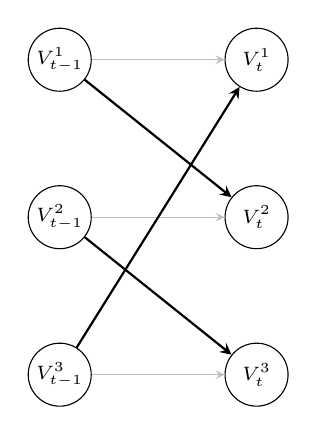
\begin{tikzpicture}[
    every node/.style={draw, circle, minimum size=0.8cm, font=\scriptsize, inner sep=0pt},
    >=stealth,
    ->,
    solidedge/.style={->, thick},
    temporal/.style={->, gray!50},
]

% t-1
\node (V1t1) at (0,4) {$V^1_{t-1}$};
\node (V2t1) at (0,2) {$V^2_{t-1}$};
\node (V3t1) at (0,0) {$V^3_{t-1}$};

% t
\node (V1t) at (2.5,4) {$V^1_t$};
\node (V2t) at (2.5,2) {$V^2_t$};
\node (V3t) at (2.5,0) {$V^3_t$};

% Temporal arrows (gray)
\foreach \i in {1,2,3} {
  \draw[temporal] (V\i t1) -- (V\i t);
}

% Causal edges (example)
\draw[solidedge] (V1t1) -- (V2t);
\draw[solidedge] (V2t1) -- (V3t);
\draw[solidedge] (V3t1) -- (V1t);

\end{tikzpicture}

\vspace{0.3em}
\textbf{(a) Lagged causal graph ($\ell_{\max}=1$)}
\end{minipage}%
\hfill
\begin{minipage}[t]{0.48\textwidth}
\centering
\vspace{0pt}
\renewcommand{\arraystretch}{1.2}
\setlength{\tabcolsep}{6pt}

\textbf{(b) Lagged adjacency tensor slice at lag \(1\)} \\[0.3em]
\(\mathbb{A}^{(0)}\)
\vspace{1.5em}

\begin{tabular}{c|ccc}
 & $V^1_{t-1}$ & $V^2_{t-1}$ & $V^3_{t-1}$ \\
\hline
$V^1_t$ & 0 & 0 & \textbf{1} \\
$V^2_t$ & \textbf{1} & 0 & 0 \\
$V^3_t$ & 0 & \textbf{1} & 0 \\
\end{tabular}

\vspace{1.5em}
%\scriptsize
\textbf{Interpretation:} $\mathbb{A}^{(0)}_{ji}=1$ indicates a directed edge $V^i_{t-1} \!\rightarrow\! V^j_t$.  For $\ell_{\max}=1$, the lag index is $\ell=0$.
\end{minipage}
\vspace{0.5em}
\caption{Illustrative example of a lagged causal graph with \(\ell_{\max}=1\) (left) and its corresponding lagged adjacency tensor (right), for a three-variable case and \(\ell_{\max}=1\). The tensor entry \(\mathbb{A}_{ji\ell_{\max}-\ell}\) indicates whether a directed causal edge from \(V^i_{t-\ell}\) to \(V^j_t\) exists. The LCM performs causal discovery by inferring \(\hat{\mathbb{A}}\), aiming to recover the true adjacency tensor \(\mathbb{A}\).}
\label{fig:lagged-tensor-example}
\end{figure}


\section{Problem Formulation} \label{sec:problem-formulation}

Formally, we seek to construct a \textit{pre-trained neural architecture capable of learning causal graphs from time-series data}. Recall from Section \ref{sec:setting} that the objective of causal discovery is to infer the underlying causal graph \( \mathcal{G} \sim \mathcal{D} \) of a dataset \( \mathcal{D} \sim \mathcal{P}_{\mathcal{D}} \). Our task is to build a \textit{large causal model} (LCM), a foundation model capable of performing causal discovery directly from time-series data, outputting a temporal causal DAG from varying input lengths, domains, and underlying causal mechanisms. Let \(\mathbf{X} = \{ \mathbf{X}_t \}_{t=1}^{n} \in \mathbb{R}^{n \times k}, \quad \mathbf{X}_t = (X_t^1, \ldots, X_t^k) \in \mathbb{R}^k\) denote a multivariate time series with \(n\) timesteps and \(k\) variables. The goal of an LCM is to infer a time-lagged causal graph that captures the directed temporal dependencies among the variables. Specifically:

%\begin{definition}[Large Causal Model]
A \textit{large causal model (LCM)} is a parametric function \(f_\theta\) mapping a multivariate time series \(\mathbf{X}\) to a \textit{lagged causal adjacency tensor}

\begin{equation}
\mathbf{X} \xrightarrow{f_\theta} \hat{\mathbb{A}},
\end{equation}

where \(\hat{\mathbb{A}} \in [0,1]^{k \times k \times \ell_{\max}}\). Each entry \(\hat{\mathbb{A}}_{j,i,\ell_{\max}-\ell}\) represents the model's confidence in the directed causal relationship \(X^i_{t-\ell} \to X^j_t\). The maximum lag \(\ell_{\max}\) is a fixed hyperparameter bounding temporal dependencies, analogous to assumptions in classical methods such as PCMCI \citep{runge2018causal}.
%\end{definition}

Unlike large language models or time-series forecasting foundation models that rely on self-supervision, causal discovery \textit{lacks natural self-supervised signals}. The ground-truth causal structure cannot be inferred from data alone, as it is fundamentally unidentifiable without external assumptions or supervision. Therefore, training follows a \textit{supervised learning scheme}, where pairs of ground truth lagged causal graphs and corresponding time-series samples are provided, generated from a known TSCM. This is illustrated in Figure \ref{fig:lagged-tensor-example}. 

As in neural networks (Figure \ref{fig:nn-train-infer}), two distinct phases are involved: (i) \textit{training}, where the model learns to map time-series data to causal graphs by provided with pairs of time-series data and their corresponding causal graphs in order to minimize its loss function; and (ii) \textit{inference (causal discovery)}, where the model (in constant time), once trained, directly outputs the predicted causal graph for unseen time-series data in the form of a lagged adjacency tensor \(\hat{\mathbb{A}}\), that best approximates the ground truth \(\mathbb{A}\). Figure \ref{fig:lcm-train-infer} conceptually illustrates the training and inference phase.

\begin{figure}[t!]
  \centering
   \makebox[\textwidth][c]{%
    \includegraphics[width=1.3\textwidth]{images/causal-foundation-model.pdf}
  }
  \caption{Training step (left) and inference (causal discovery) step (right) of a large causal model \(f_\theta\), represented as a sequence of blocks. During training, the model learns to map input time-series \(\mathbf{X}\) to causal graphs by minimizing a supervised loss between the predicted graph \(\mathcal{G}_{\text{pred}}\) and ground-truth \(\mathcal{G}_{\text{gt}}\). During inference, the pre-trained model directly outputs \(\mathcal{G}_{\text{pred}}\) for unseen inputs.}
  \label{fig:lcm-train-infer}
\end{figure}

To make the problem well-posed under a supervised learning setting, we assume (i) sufficient overlap between training and test distributions \citep{ke2023learning, stein2024embracing, wu2024sample}, (ii) causal assumptions (described in Table \ref{tab:causal-assumptions}), and (iii) bounded temporal dependencies via fixed \(\ell_{\max}\). This formulation highlights the need for large and diverse training collections of temporal data and their corresponding causal graphs. In practice, \(\hat{\mathbb{A}}\) corresponds to a \textit{soft prediction tensor}: it assigns a confidence score to each potential lagged edge rather than a hard decision. To evaluate performance against the ground truth, these scores are binarized via a thresholding operator \(\hat{\mathcal{G}} = 1\{\hat{\mathbb{A}} \geq \tau\}\) (elaborated in Chapter \ref{chap:training}). Different values of \(\tau\) yield different precision-recall trade-offs, summarized using ROC/AUC and related metrics in Chapter \ref{chap:results}. Additionally, in order to handle samples and TSCMs of varying number of samples, variables and lags, a padding mechanism must be implemented as in conventional foundation models. A thorough discussion of the above is provided in Chapter \ref{chap:architecture}.
	%\chapter{Data Generation} \label{chap:data}

\begin{chapquote}{\textit{Abraham Lincoln}}
``If I had six hours to chop down a tree, I'd spend the first four sharpening the axe.''
\end{chapquote}

A central limitation of current causal discovery methods, either in the temporal or i.i.d. setting, is the exclusive reliance on synthetic datasets for their evaluation, benchmarking and recently, for foundational-inspired methods (Section \ref{sec:related-work}), training. This chapter outlines our methodologies for generating vast data instances\footnote{We refer to a pair of a multivariate time-series and its corresponding causal graph as a \textit{data instance} or simply dataset, when no ambiguity exists regarding the form of data. Multiple pairs of data instances are referred to as a \textit{data collection.}} to support robust training of our large causal models. Synthetic data generation pipelines are typically constructed using predefined causal structures and known functional dependencies from randomly generated SCMs. While such approaches offer precise control and clarity over the data generation process, they often fail to capture the complexity and statistical idiosyncrasies of real-world time-series. To address this, we propose generation methods of both \textit{synthetic} and \textit{simulated} (realistically generated) data. Briefly, we opt for training on a mixture of both synthetic and simulated datasets. 

We begin with an introduction to the context of data generation (Section \ref{sec:data-introduction}) and proceed by outlining the main challenges for causal discovery (Section \ref{sec:data-challenge}). The remainder is structured as follows: Section \ref{sec:data-synthetic} outlines the generation process of synthetic data pairs, which serve as a learning foundation for our Large Causal Models. Section \ref{sec:data-simulated} introduces the \textit{Temporal Causal-based Simulation (TCS)} framework, a modular and model-agnostic generative method for causal models and corresponding time-series samples, as well as the \textit{Adversarial Causal Tuning (ACT)} module, which enables fine-tuning of TCS based on a Min-max optimization approach. Unlike traditional synthetic data generators in literature, our methodology learns the structural and functional dependencies, as well as the noise distribution, directly from time-series samples, and by allowing fine-tuning of the process further enhances the realism of generated causal models and bridges the domain gap between synthetic training and applicability to real-world scenarios. This part serves as a crucial component for enhancing the generalization performance of our LCMs, allowing us to leverage data of higher quality for not only training, but also evaluation and benchmarking. Section \ref{sec:data-training} covers the curation of training and validation pairs used for model training, as well as the construction of our benchmark datasets. Finally, Section \ref{subsec:shardification} provides an overview of our approach for partitioning data into shards for efficient training of LCMs.

\section{Introduction} \label{sec:data-introduction}

In the foundation model paradigm, model performance and generalization is closely tied to training data quality and diversity \citep{bommasani2021opportunities}. In the same way foundation models for natural language processing (e.g. Large Language Models-LLMs like the family of GPTs \citep{radford2019language, brown2020language, achiam2023gpt}) and computer vision (e.g. CLIP \citep{radford2021learning}, DALL-E \citep{ramesh2021zero}) rely on vast and heterogeneous data collections to fully capture the complexities of the real world in order to generalize effectively, a foundation model for causal discovery would require training data that reflect the complexities and properties of real-world causal systems.

For the most part, obtaining real data-cases is a straightforward task for domains unrelated to causality. Consider for example the case of constructing a neural model for recognizing images (such as dogs, cats, a glass bottle etc.). Real-world images are widely available online and can even be collected easily nowadays. For a supervised learning like image classification, it is then a matter of \textit{annotating} each image with its ground truth label. Such labeled image collections have already been curated, such as Imagenet \citep{deng2009imagenet}. A similar scenario exists for time-series forecasting models as well \citep{hahn2023time, kim2025comprehensive}. Foundation models for time-series forecasting have been developed and trained on such data collections, such as the Transformer XL \citep{dai2019transformer}, the Informer \citep{zhou2021informer} etc.

An ongoing challenge in causal discovery is obtaining real data-cases, as it represents a much more nuanced task that generating purely synthetic ones. In the absence of real-world data and causal graph pairs, existing works regarding causal discovery on both \textit{iid} and temporal data tend to focus on using either on (i) \textit{purely synthetic} samples (causal models with randomized Erd\H{o}s-Renyi \citep{brouillard2020differentiable} or Barab\'{a}si-Albert \citep{barabasi1999emergence} structures) or (ii) \textit{semi-synthetic}, based on existing knowledge of real cases and scenarios (e.g., simulated Markov processes of physical systems). Examples of such datasets include the Kuramoto model of coupled oscillators \citep{kuramoto1975self, lowe2022amortized} and brain connectivity models such as \(f\)MRI \citep{smith2011network}. Observational data from synthetic causal models are then generated through \textit{ancestral sampling} \citep[Section 4.2.5]{murphy2023probabilistic} from the specified temporal SCM, and interventional data, if needed, in a similar manner. While this approach provides full control over the form of the causal structure and resulting causations, it leads to inherent limitations: synthetic data generation operates under idealized assumptions, including fully specified models, simplified noise distributions, absence of latent confounding, noisy interactions etc. As a result, generated data often fail to capture the complexity, heterogeneity, and non-stationary characteristics of real-world time-series. Real time-series samples are vastly available, but each one must be accompanied with its ground truth causal mechanism, from which data samples are generated from. As many causal assumptions on which causal discovery and causal inference methods are built upon (as elaborated in Chapter \ref{chap:problem-formulation}) are unknown or unlikely to hold in such real-world systems, the need for realistic data cases is even more pressing.

Regarding training of foundation models, the authors of TimesFM \citep{das2024decoder} articulate this principle clearly in the context of time-series forecasting: \\

\begin{chapquote}{\textit{Rajat Sen and Yichen Zhou}, TimesFM authors\footnote{\url{https://research.google/blog/a-decoder-only-foundation-model-for-time-series-forecasting} (Last Accessed: May 2025).}}
``Synthetic data helps with the basics... Real-world data adds real-world flavor... This helps TimesFM understand the bigger picture and generalize better when provided with domain-specific contexts not seen during training.''
\end{chapquote}

This sharp observation holds equally true for foundation models for causal discovery: synthetic data encode fundamental structural and temporal dependencies, while realistic data capture the statistical irregularities and intractable functional complexities inherent in real-world systems.

Surprisingly, causal discovery methods, including recent foundation models presented in Section \ref{sec:related-work} such as CP \citep{stein2024embracing}, SEA \citep{wu2024sample} and Do-PFN \citep{robertson2025do} are trained exclusively on synthetic datasets. Such models are rarely exposed to the structural uncertainty, noise variability or irregular patterns present in real data. Furthermore, their evaluation is typically restricted to synthetic benchmarks, limiting their demonstrated generalization capacity in practical deployment scenarios.

To address the above concerns, our work adopts a dual-strategy approach for data generation. Alongside a conventional yet rigid synthetic data generation pipeline from temporal SCMs, we introduce realistically generated datasets constructed using Adversarial Causal Tuning - ACT, inspired by AutoML \citep{hutter2019automated}. In short, the method generates time-series and corresponding lagged causal graphs by learning directly from real data samples. It decomposes the data generation process into three modular phases: (i) discovery of the causal graph, (ii) approximation of the functional dependencies and (iii) noise distribution modeling, all under a Min-max fine tuning scheme for optimal causal model selection. In this way, we allow generation of time-series that are both causally coherent and statistically realistic.

%To address the above concerns, our work adopts a dual-strategy approach for data generation. Alongside a conventional yet rigid synthetic data generation pipeline from temporal SCMs, we introduce realistically generated datasets constructed using the \textit{Temporal Causal-based Simulation} (TCS) framework. TCS generates time-series and corresponding lagged causal graphs by learning directly from real data samples. In short, it decomposes the data generation process into three modular phases: (i) discovery of the causal graph, (ii) approximation of the functional dependencies and (iii) noise distribution modeling, all under a Min-max fine tuning scheme for optimal causal model selection (\textit{Adversarial Causal Tuning - ACT}) inspired by AutoML \citep{hutter2019automated}. In this way, we allow generation of time-series that are both causally coherent and statistically realistic.

\section{The Challenge} \label{sec:data-challenge}

The task of generating synthetic instances is evidently a more straightforward problem than the one of generating realistic ones. Various works that address synthetic causal data generation have been introduced, in both temporal and atemporal settings \citep{cinquini2021boosting, wen2021causal}, yet few assess the realism and quality of generated data. Concerning time-series, methods taking into account sophisticated and configurable generative frameworks for both data and the causal structure itself exist (such as \cite{lawrence2020cdml}). Methods such as Causal Chambers by \citet{gamella2024causal} for generating realistic time-series data from physical systems under controlled experimental conditions have also been recently introduced. A key difference between our approach and theirs is that our proposed pipeline remains fully algorithmic, enabling scalable and diverse data generation, instead of a closed and controlled experimental setup. The work of \citet{stein2024embracing} also includes a synthetic generator of time-series, as well as the Tigramite package by \cite{runge2019inferring}. A shortcoming of these works is that during ancestral sampling over the causal graph, cuasal effects may grow too large due to the functional relationships used, thus resulting in values outside floating point range. This issue is handled by re-instantiating the sampling process, which can prove time consuming and cumbersome for generating thousands of instances. What's more, some chosen functional relationships or parametric assumptions about the noise distributions may result in causal graphs that are either too trivial for the model to generalize or too hard for the model to extract any meaningful context. Furthermore, the work of \citet{stein2024embracing}, although it follows an additive time-invariant SCM formulation for samples, it directly proceeds by randomly populating the lagged adjacency tensor, which remains of questionable soundness, as no TSCM is directly introduced. Finally, graphs may prove to be too dense (causal graphs should be, in general, sparse), which may lead the model to either overfit or underfit the data. We take into consideration the above points for the introduction of our own synthetic generation pipeline to output coherent time-lagged causal graphs for training and evaluation of our LCMs.

In the case of real-world data, the challenge is much more complex. The main argument against the sole use of synthetic dta is that reliance on data generated under idealized assumptions, e.g., additive noise models, pre-defined structural priors, or linear interactions, limits data quality and as such the generalization capabilities of our LCMs (i.e. Figure \ref{fig:stein_fmri} in Chapter \ref{chap:introduction}). As we elaborate in detail in Section \ref{sec:data-simulated}, common evaluation protocols for realistic data generators use single-metric comparisons \citep{cheng2024causaltime}, which do not fully capture the generative realism or causal fidelity. What's more, assumptions of both purely synthetic and semi-synthetic causally generated data are unlikely to hold in practice, as real-world models are subject to inherent restrictions and do not fit under closed conditions assumed by such methods. Generating datasets that are both causally coherent and statistically realistic remains a core challenge addressed in this work. We call such datasets \textit{simulated} data.

The assumption (stemming from adopting a supervised learning approach as elaborated in Section \ref{sec:problem-formulation}), that \textit{distributions of training and test data cases must highly overlap}, poses another fundamental challenge in data generation. As one may expect, a supervised classification model (not limited to a neural network) trained on linear instances is expected to perform poorly on non-linear cases. This simple observations further highlights the need for \textit{curating a large data collection with various complexities, sizes and causal properties for training and evaluation}. For synthetic cases, this includes a wide family of graph sizes, node degrees, functional relationships and noise distributions, among others. 

To extend the limited dimensionality from five (\(5\)) variables of \citet{stein2024embracing} to more than double (twelve (\(12\))), the need for constructing an optimal curation of both synthetic and simulated data remains even more significant. The challenge of constructing a vast collection of data (among other number of variables, lags of causal relationships, functional dependencies etc.) is evident in order to avoid degradation of model performance as input dimensionality and model parameters increase (Figure \ref{fig:stein_auc} in Chapter \ref{chap:introduction}).

Finally, one should be accounting for causal assumptions that are not only reflected in the training data but also in the assumptions of the model. For instance, consider generating observational samples from a causal structure \(X_{t} \leftarrow Z_{t-1} \rightarrow Y_{t}\) where \(Z\) is assumed to be a latent confounder and then removed from the corresponding SCM. A model that assumes causal sufficiency would potentially infer (based on these observational samples) a directed edge between \(X_t\) and \(Y_{t}\) (of any lag), which clearly is not the case and results in false interpretation of discovered causal relationships.

\section{Generating Synthetic Causal Models} \label{sec:data-synthetic}

Recall from Chapter \ref{chap:problem-formulation} that we formulate causal mechanisms as a (temporal) SCM, represented by a tuple \((\mathcal{G}, \mathcal{F}, \mathcal{E})\), where \(\mathcal{G}\) is the causal DAG (TSCM), \(\mathcal{F}\) the set of functional dependencies, and \(\mathcal{E}\) the set of noise distributions. Loosely speaking, a generator of random TSCMs and observational samples thus consists of a two-step process. First, a causal DAG instance \(\mathcal{G}\) is sampled from a predefined family of DAGs \(\mathbb{G}\) with various random properties. These may include the number of nodes, edge density (e.g., in-degree and out-degree distributions), the maximum number of lags \(\ell_\text{max}\) in the case of temporal SCMs, and the overall graph structure (e.g., uniform distribution of degrees). With the causal structure known, functional dependencies \( f_i = f(V^i_t | \text{Pa}(V^i_t))\) are sampled for each \(X_i \in \mathcal{G}\) given its parents in the DAG, from known functional families \(\mathcal{F}_1, \ldots,\mathcal{F}_k\), along with noise distributions \( \epsilon_i \sim \mathcal{E}_1, \ldots, \mathcal{E}_m\). For nodes \(V^i_t\) where \(\text{Pa}(V^i_t) = \emptyset\), values are sampled directly from the assumed noise distribution. With both the causal structure and quantitative dependencies defined, the second step consists of generating samples from the SCM.

To illustrate sample generation, consider a simple i.i.d. example with three variables \(X, Y, Z\) and the causal DAG described by the collider \(X \rightarrow Z \leftarrow Y\). This causal graph is associated with the functional dependency \(Z := f(X,Y,\epsilon_Z)\) and noise distributions \(X \sim \epsilon_X\), \(Y \sim \epsilon_Y\). Observational samples are obtained by respecting the topological order of the DAG and generating samples recursively over the descendants (similar to ancestral sampling in latent variable models \citep{murphy2023probabilistic}). For instance, one sample may be \(X = 0.02, Y=0.12\) and \(Z = f(0.02,0.12,0.03) = 1\), where values from the noise distributions are substituted into the functional dependencies.

The topology of each synthetic SCM depends on the random graph generation method. Two main methods exist for random DAG generation in the literature. The first follows the \textit{Erd\H{o}s-Renyi (ER)} paradigm \citep{fienberg2012brief}, as in \citet{hagberg2008exploring}, with variations also used by \citet{brouillard2020differentiable} and \citet{ke2022learning}. Generation begins with an empty graph for a given number of nodes, then randomly and equiprobably picks directed edges to add based on a probability \(p\). Unlike \citet{hagberg2008exploring}, acyclicity checks are applied to reject edges that would introduce cycles, as shown in Algorithm \ref{alg:erdos-renyi}. This process produces approximately uniform node degree distributions.

The second approach, the \textit{Barab{\'a}si-Albert (BA)} algorithm \citep{hagberg2008exploring,barabasi1999emergence}, generates scale-free graphs whose degree distribution follows a power law. Such networks exhibit a “rich-get-richer” phenomenon where a few nodes accumulate disproportionately many connections, a property often seen in real-world networks like social graphs.

In our experiments, we adopt the \textit{Erd\H{o}s-Renyi} method for generating \textit{random lagged temporal causal graphs} (Figure \ref{fig:temporal-graphs} (a)), as it allows fine-grained control over edge probabilities and density. In time-series settings, the additional temporal dimension must be considered. Since we are interested in lagged causal graphs, Algorithm \ref{alg:erdos-renyi} is adapted as follows: the number of nodes \(V\) is sampled from a discrete uniform distribution \(\mathcal{U}(V_\text{min}, V_\text{max})\), the edge probability \(p\) from \(\mathcal{U}(0, 1)\), and the maximum causal effect lag \(\ell_\text{max}\) from \(\mathcal{U}(1, \ell_\text{max})\). The resulting time-lagged graph contains \(V \cdot \ell_\text{max}\) lagged nodes at timesteps \(\tau=1, \dots, \ell_\text{max}\) and \(V\) nodes at the current timestep \(\tau=t\). Directed edges (heading forward through time) are added randomly according to the chosen \(p\), ensuring acyclicity. Furthermore, \textit{no contemporaneous edges are assumed}, i.e., edges of the form \(V^i_l - V^j_l\) do not exist.

The \textit{Barab{\'a}si-Albert} model, while useful for studying scale-free networks, tends to create overly connected hubs that are less representative of causal graphs in scientific domains, and is therefore left unconsidered.

 \begin{algorithm}
 \caption{Erd\H{o}s-R\'{e}nyi DAG generator} \label{alg:erdos-renyi}
 \begin{algorithmic} [1]
 \renewcommand{\algorithmicrequire}{\textbf{Input:}}
 \renewcommand{\algorithmicensure}{\textbf{Output:}}
 \REQUIRE $n$, $p$
 \ENSURE  a DAG $\mathcal{G}$
  \STATE initialize $\mathcal{G}$, $\mathcal{G}^{'}$ as empty directed graphs with $n$ nodes
  \STATE initialize $edges$ with all the possible directed arcs in $\mathcal{G}$, $m=n \cdot p$
\WHILE {$|edges|>0$ and (number of edges in $\mathcal{G} \le m$)}
    \STATE $e \leftarrow \text{pop(shuffle(edges))}$
    \IF {$p \le$ random uniform sample in $[0,1]$}
        \STATE $D \leftarrow \mathcal{G}^{'}$
        \STATE add $e$ to $D$
        \IF {$V$ has a cycle}
            \STATE $D \leftarrow \mathcal{G}^{'}$
        \ELSE 
            \STATE add $e$ to $\mathcal{G}$
            \STATE add $e$ to $\mathcal{G}^{'}$
        \ENDIF
    \ENDIF
\ENDWHILE
\RETURN $\mathcal{G}$ 
\end{algorithmic}
\end{algorithm}

After generating the DAG structure with the desired properties, functional dependencies \(f^j (\text{Pa}( V^j_t), \epsilon^j_t)\) for each variable \(V^j_t \in \mathcal{G}\) are sampled from known functional families \(\mathcal{F}_1, \ldots, \mathcal{F}_k\), along with the corresponding noise distributions. This finalizes the SCM, from which observational data can be sampled.

Generation of samples is carried out using causal ancestral sampling, similar to ancestral sampling in latent variable models (LVMs) \citep{murphy2023probabilistic}. In short, variables without parents are sampled from their noise distributions, and variables with parents are computed from their functional dependencies, respecting topological order. In the temporal case, parent variables are fetched from lagged causal parents, and initial “warm-up” samples are discarded to ensure stability in the generated time-series, following \citet{runge2018causal}. Assuming a known time-lagged SCM \(\mathcal{G}\) with maximum lag \(\ell_{\text{max}}\), the process is described in Algorithm \ref{alg:scm-ancestral-sampling}.

\begin{algorithm}[ht!]
\caption{Temporal SCM Ancestral Sampling (ANCESTRAL)}
\label{alg:scm-ancestral-sampling}
\begin{algorithmic}[1]
\renewcommand{\algorithmicrequire}{\textbf{Input:}}
\renewcommand{\algorithmicensure}{\textbf{Output:}}
\REQUIRE{Temporal Causal Graph \( \mathcal{G} \), max lag \( \ell_\text{max} \), number of timesteps \( T \), number of warmup steps \( W \)}
\ENSURE Generated time-series $\{\mathbf{X}_t\}_{t=1}^{T}$
\STATE Initialize $X^i_{t=0}$ for all $i \in \{1, \dots, N\}$ with random noise
\FOR{$t = W + \ell_{\text{max}} + 1$ to $T$}
    \FOR{each variable $X^i_t$ in topological order of $\mathcal{G}$}
        \STATE Determine lagged parents $\mathrm{Pa}_{X^i_t} \gets \{X^j_{t-k} \mid (X^j, X^i) \in \mathcal{G}, 1 \leq k \leq \ell_{\text{max}}\}$
        \STATE Compute $X^i_t \gets f_i(\mathrm{Pa}_{X^i_t}) + \epsilon^i_t$
    \ENDFOR
\ENDFOR
\RETURN $\{\mathbf{X}^i_t\}_{W+\ell_{\text{max}}}^{T}$
\end{algorithmic}
\end{algorithm}

We now elaborate on the generation hyperparameters used for synthetic sample creation. We select \(V_\text{min}=3, V_\text{max}=12\) and \(\ell_{\text{max}} = 3\). Two-variable SCMs are trivial under our assumptions (edges move forward in time and no latent confounders exist). The choice \(V_{\max}=12\) more than doubles the dimensionality of current state-of-the-art datasets, while \(\ell_{\max}=3\) balances (i) realism in short-term dependencies and (ii) tractability in training. Sampling graphs up to these limits aligns with the design constraints of our LCMs (as discussed in Section \ref{sec:problem-formulation} and Chapter \ref{chap:architecture}). A summary of these parameters is shown in Table \ref{tab:scm-parameters}.

\begin{table}[h]
\centering
\caption{Summary of synthetic SCM generation parameters.} \label{tab:scm-parameters}
\begin{tabular}{lllp{5cm}}
\toprule
\textbf{Parameter} & \textbf{Range / Values} & \textbf{Sampling}\\
\midrule
\# Variables \( N \) & 3 to 12 & Uniform discrete \\
\# Lags \( \ell_{\max} \) & 1 to 3 & Uniform discrete \\
Functional dependencies & See Table \ref{tab:functions} & Uniform discrete \\
Noise distributions & See Table \ref{tab:noise-dists} & Categorical \\
Edge probabilities \( p_{\text{edge}} \) & Dynamic & Categorical \\
\bottomrule
\end{tabular}
\end{table}

To prevent pathological graph densities, \(p_\text{edge}\) is scaled adaptively to the number of possible lagged edges \(E=N^2 \cdot \ell_{\max}\). Specifically, \(p_\text{edge}\) is sampled from a discrete set of values inversely proportional to \(E\), with categorical weights favoring sparsity (Table \ref{tab:p-edge-ranges}). If no edges are sampled during graph generation, \(p_\text{edge}\) is iteratively increased by \(1\%\) until a valid graph is obtained. This dynamic adjustment ensures diversity across sparse, medium, and dense regimes while maintaining realism. Additionally, \(p_\text{edge}\) is upper bounded by \(0.15\) to avoid dense graphs.

\begin{table}[h]
\centering
\caption{Functional dependencies used in synthetic SCM generation.} \label{tab:functions}
\begin{tabular}{lll}
\toprule
\textbf{Family} & \textbf{Functional form} & \textbf{Description} \\
\midrule
Linear & \(f(x) = a x + b\); & Additive linear effect \\
       & \(f(x_1, x_2) = a_1 x_1 + a_2 x_2 + b\) & Linear combination of parents \\
\midrule
Non-linear & \(f(x) = \alpha_nx^n + \ldots \alpha_0x_0 \); & Polynomial \\
           & \(f(x) = e^x \); & Exponential Transformation \\
           & \(f(x) = \sin(x)\); & Sinusoidal \\
           & \(f(x_1, x_2) = x_1 x_2\); & Multiplicative interaction \\
           & \(f(x) = \log(1 + |x|)\); & Logarithmic transformation \\
\midrule
Bounded & \( f(x) = \tanh(x) \) & Hyperbolic tangent (bounded in \([-1,1]\)) \\
        & \( f(x) = \sigma(x) \) & Sigmoid \( \big(\frac{1}{1+e^{-x}}\big) \) \\
\bottomrule
\end{tabular}
\end{table}

\begin{table}[h]
\centering
\caption{Noise distributions used in synthetic SCMs.} \label{tab:noise-dists}
\begin{tabular}{lll}
\toprule
\textbf{Name} & \textbf{Distribution} & \textbf{Parameters} \\
\midrule
Gaussian & \( \mathcal{N}(\mu, \sigma^2) \) & \(\mu=0, \sigma=0.25\)\\
Uniform & \( \mathcal{U}(a, b) \) & \( a=0, b=1 \) \\
\bottomrule
\end{tabular}
\end{table}

Functional forms include linear, polynomial, multiplicative, bounded, and sinusoidal mappings, selected from Table \ref{tab:functions}. Each causal edge is assigned a strength coefficient \(\alpha_{ji\lambda} \sim \mathcal{U}(0.3, 0.5)\), controlling the contribution of each parent variable. These coefficients populate the nonzero entries of the lagged adjacency tensor \(\mathbb{A} \in \mathbb{R}^{V \times V \times \ell_{\text{max}}}\), interpreted as edge-level causal strengths rather than causal effect estimates. Noise distributions are sampled from those listed in Table \ref{tab:noise-dists}.

Finally, each synthetic sample is padded or truncated to a fixed sequence length \(L_\text{max}=500\) and variable dimension \(V_\text{max}=12\) to ensure batch processing and model input compatibility (see Section \ref{sec:input-handling}).

\begin{table}[h]
\centering
\caption{Edge probability values used for different synthetic causal graph densities. \(E\) denotes the number of possible lagged edges.} \label{tab:p-edge-ranges}
\begin{tabular}{ccccl}
\toprule
\textbf{Edge Regime} & \textbf{Threshold} & \textbf{Values} & \textbf{Weights} & \textbf{Notes} \\
\midrule
Small graphs & \( E < 100 \) & \( \frac{3}{E}, \frac{5}{E}, \frac{7}{E} \) & \( 0.6, 0.3, 0.1 \) & Promotes sparsity \\
Medium graphs & \( 100 \le E < 200 \) & \( \frac{5}{E}, \frac{7}{E}, \frac{9}{E} \) & \( 0.6, 0.3, 0.1 \) & Moderate edge density \\
Large graphs & \( E \ge 200 \) & \( \frac{9}{E}, \frac{12}{E}, \frac{15}{E} \) & \( 0.6, 0.3, 0.1 \) & Higher density permitted \\
\bottomrule
\end{tabular}
\end{table}

\section{Generating Simulated  Pairs} \label{sec:data-simulated}

In contrast to synthetic data, simulated (realistically generated) data aim to reflect the underlying causal dynamics of real-world systems by reverse-engineering the structural and functional dependencies from actual time-series. Essentially, we address the problem of generating time-series data from a causal model with the same distribution as a given real dataset, that is, constructing a probabilistic causal digital twin. 

For this purpose, we introduce the \textit{Temporal Causal-based Simulation (TCS)} framework, a modular and model-agnostic generative \footnote{A generative model is a type of machine learning model designed to learn the underlying probability distribution of a dataset and is therefore capable of generating new, synthetic data samples that are statistically and structurally similar to the training data.} method for generating time-series along with their temporal causal graphs, which incorporates a fine-tuning process for optimal model selection called \textit{Adversarial Causal Tuning (ACT)}. Generated data is not only statistically coherent but also maintains interpretable causal consistency, making it suitable for training and benchmarking of our Large Causal Models.

Ideally, what one is looking for is the ability to generate data that is both realistic and comparable to real-world cases, and as such a way to discrimimate between simulated data of good and poor quality. In literature, there exist various methods for asserting whether two data samples resemble each other. One way to measure similarity between (observed) real and synthetic data is by the \textit{Maximum Mean Discrepancy (MMD)} \citep{gretton2006kernel} metric. MMD measures the distance between two probability distributions by embedding the data into a reproducing kernel inner-product space and calculating the difference in the mean embeddings. The MMD score is given by \(\text{MMD}^2(X, Y) = \mathbb{E}_{X, X}[k(X, X)] + \mathbb{E}_{Y, Y}[k(Y, Y)] - 2\mathbb{E}_{X, Y}[k(X, Y)]\), where \(X\) and \(Y\) are the real and synthetic data samples respectively and the expectations are taken over all points in the selected data batch. 

A more useful way to assess data similarity is using \textit{Classifier 2-sample tests (C2STs)}. The main idea behind C2STs, introduced by \citet{gretton2012kernel}, is to train a machine learning classifier \(f_\theta\) to distinguish samples \(X=\left\{x_1,\ldots,x_n\right\} \) sampled from distribution \(P\) against samples \(Y = \left\{y_1,\ldots,y_m\right\}\) sampled from distribution \(Q\). Intuitively, if the null hypothesis \(H_0: P = Q\) holds, then the classifier (trained on the labeled training set \(\mathcal{D} = \left\{ (x_i, 0)\right\} \cup \left\{ (y_j, 1)\right\}\)) should be unable to distinguish between samples and should demonstrate performance close to \(1/2\), or chance level when evaluated on a holdout test set. By performance, we refer to the AUC-ROC score of the classifier \citep{bradley1997use}, to which we refer to as \textit{discrimimation score} \(\mathrm{AUC}_D\). As \citet{lopez2017revisiting} demonstrated, classifier 2-sample tests offer several attractive properties for evaluating data similarity, such as assessing the quality of samples generated by models where the likelihood is intractable (cannot be computed analytically) but sampling from the generating process is tractable.

To highlight our contributions in realistic data generation, we present key arguments against the suitability of the work by \citet{cheng2024causaltime} for training and evaluating our LCMs. It remains the closest to our work, in the sense that it is applicable to time-series and has been introduced as a method to benchmark causal discovery algorithms. However, it faces several shortcomings. It begins by fitting a residual-based neural network (\textit{causally disentangled neural network - CDNN}), based on either an MLP or an LSTM architecture, to model a \textit{vector autoRegressive (VAR)} process, using all historical variables for a specified maximum lag; it then extracts a \textit{hypothetical causal graph (HCG)} based on computed feature importance values, using methods such as deep Shapley additive exPlanations (DeepSHAP) \citep{lundberg2017unified}, while being able to generate data auto-regressively from the fitted model. As the authors themselves point out throughout their paper, the extracted HCG using feature importance does not constitute causal discovery and does not represent a causal model. As such, causal queries are not possible and the discovered graph does not represent a causal digital twin. As their extracted hypothetical causal graph represents a \textit{summary graph} with no lag information and not a \textit{lagged causal graph} (Figure \ref{fig:temporal-graphs}), its scope remains limited. Additionally, although a generative mechanism for data exists by the fitted model, it does not reflect or approximate the underlying TSCM mechanism. Consequently, generation of interventional samples is unfeasible: the resulting process may generate temporally correlated samples, but not reason causally, e.g. to estimate \(P(Y|\text{do}(X=x))\). 

\begin{figure}[ht!]
    \centering
    \begin{minipage}[t]{0.32\textwidth}
        \centering
        \includegraphics[width=0.99\linewidth]{images/figures/t-a.png}
        \label{fig:tsne-a}
    \end{minipage}%
    \hfill
    \begin{minipage}[t]{0.32\textwidth}
        \centering
        \includegraphics[width=0.99\linewidth]{images/figures/t-b.png}
        \label{fig:tsne-b}
    \end{minipage}%
    \hfill
    \begin{minipage}[t]{0.32\textwidth}
        \centering
        \includegraphics[width=0.99\linewidth]{images/figures/t-c.png}
        \label{fig:tsne-c}
    \end{minipage}

    \vspace{15pt}

    \caption{t-SNE \citep{maaten2008visualizing} projections of original and simulated data across different datasets. Optimized C2ST variants outperform standard methods (e.g., MMD) in detecting distributional differences, even when visual separability is low.}
    \label{fig:tsne}

    \vspace{15pt}
\end{figure}

Furthermore, CausalTime relies on a single discriminator to evaluate its simulation quality in addition to the MMD metric. As shown in Figure \ref{fig:tsne} leads to misleading conclusions about the quality of generated data. Data are projected in the plane using t-SNE \citep{maaten2008visualizing}, and the discriminator is trained to distinguish between real and generated data. In Figure \ref{fig:tsne} (a), only the support vector classifier (SVC)-based C2ST is able to distinguish simulated from original samples, which have been generated using trigonometric functions. The other two C2STs, based on logistic regression (LR) and long-short-term memory (LSTM) are unable to do so, with an \(\mathrm{AUC}_D\) of \(0.52\) and \(0.61\) respectively. A similar experimental scenario is shown in Figure \ref{fig:tsne} (b) on the \texttt{AirQualityUCI} dataset where an optimized\footnote{An optimized classifier refers to a model whose hyperparameters or configuration are tuned to maximize its performance (e.g., \(\mathrm{AUC}_D\)), whereas an unoptimized classifier uses default or untuned parameters.} LSTM classifier discriminates, while the unoptimized one fails. Finally, Figure \ref{fig:tsne} (c) reveals the inadequacy of the maximum mean discrepancy metric, as although it is close to zero and data seem indistinguishable with the naked eye, an optimized LSTM classifier is still able to separate them. Consequently, the need for introducing a causal model generator by utilizing optimized C2STs is clear.

\subsection{Temporal Causal-based Simulation (TCS)} \label{subsec:tcs}

This subsection is dedicated to the main generative method for producing realistic time-series data and their respective time-lagged causal graph, called \textit{Temporal Causal-based Simulation (TCS)}, depicted in Figure \ref{fig:pipeline-part-a}. Our method can be summarized briefly by the following statement: \textit{Select the model that generates simulated data which, despite our best efforts, are indistinguishable from the real training data}. By best efforts, we refer to the fine-tuning phase. We summarize the formulation as follows: (i) a \textit{Generation phase}, where a module performs a search in the space of causal models by generating TSCMs and (ii) a \textit{Tuning phase}, where another module searches the space of discriminators to distinguish between real and simulated data, called \textit{Adversarial Causal Tuning (ACT)}. The above procedure leads to a Min-max selection scheme, similarly to generative adversarial networks (GANs) \citep{goodfellow2014generative}. We now describe the main phases of the TSCM search space and ACT.

\begin{figure}[tbp]
    \centering
    \includegraphics[width=\textwidth]{images/figures/pipeline_aaa.png}
    \caption{
        Given a multivariate time-series sample of real data, the method begins by estimating the lagged causal graph through temporal causal discovery (\textit{Phase 1}). It then estimates the functional dependencies between variables using a wide range of forecasters (\textit{Phase 2}). Based on the predictions of these forecasters, it learns the noise distribution through a variety of density estimation methods (\textit{Phase 3}). Each combination of methods for Phases 1, 2 and 3 constitutes a configuration for TCS, that results in a unique \textit{temporal causal model}. By considering different configurations, TCS creates a search space for the temporal causal model that best describes the real data.
    }
    \label{fig:pipeline-part-a}
\end{figure}

\subsubsection{Generation of TSCMs}

\paragraph{Phase 1: Causal Discovery}

Initially, TCS retrieves the data's causal structure. To achieve this, the method employs a variety of causal discovery methods for temporal data, either established as a gold standard or express the current state-of-the-art. Specifically, we consider the algorithms \textit{PCMCI} \citep{runge2018causal} and \textit{DYNOTEARS} \citep{pamfil2020dynotears}. PCMCI is a CD method based on conditional independence testing, serving as a temporal extension of PC \citep{spirtes2001causation} established through literature, while DYNOTEARS constitutes an extension of the NOTEARS \citep{zheng2018dags} CD algorithm on temporal data, based on continuous optimization. These methods are also used as benchmarks for evaluating our trained LCMs and are discussed in detail at Section \ref{sec:baselines}.

We now describe the generation of TSCMs with some mathematical rigor. Given a multivariate time-series dataset \( \mathcal{D} \) over \( \mathbf{V} \), the first phase performs temporal causal discovery using an CD algorithm dependent on a given parameter configuration \( \mathbf{B}_\text{CD} \) (e.g. for DYNOTEARS, the regularization constants \( \lambda_\mathbf{W}, \lambda_\mathbf{A} \in \mathbf{B}_\text{CD} \)). That is, obtain: 

\begin{equation}\label{eq:phase-cd}
\mathcal{G}, \left\{ \mathbf{Pa}_{X^i} \right\}_{i \in \mathbf{V}} \leftarrow \text{CAUSAL\_ALG}(\mathcal{D}, \mathbf{B}_\text{CD})
\end{equation}

It is crucial to highlight that the outcome of all the considered time-series CD methods are \textit{lagged causal graphs}, that not only serve as an expressive representation of the causal model for training our LCMs, but also able to preserve the temporal structure of data for further use. We describe TCS in Algorithm \ref{alg:tcs}. It should also be noted that as causal discovery algorithms are governed by a set of causal assumptions, sampled data from TCS, as well as input data to the method, are assumed to follow these assumptions. The algorithms and their assumptions are selected to align with the causal assumptions of our LCMs, in Chapter \ref{chap:architecture}. 

\begin{algorithm}[t]
\caption{Temporal Causal-Based Simulation (TCS-SIMULATE)}
\label{alg:tcs}
\begin{algorithmic}[1]
\renewcommand{\algorithmicrequire}{\textbf{Input:}}
\renewcommand{\algorithmicensure}{\textbf{Output:}}
\REQUIRE Real time-series dataset $\mathcal{D} = \{\mathbf{X}_t\}_{t=1}^{T}$ over variable set $\mathbf{V}$; sample size $n$; causal discovery configs $\{\mathbf{B}_{CD}\}$; functional dependency estimator configs $\{\mathbf{B}_{pred}\}$; noise estimation configs $\{\mathbf{B}_{noise}\}$; ACT parameters $(D, \{C_d\}, \alpha, n_{perm})$
\ENSURE Optimal causal model $s_{\text{best}}$, generated dataset $\mathcal{D}'_{s_{\text{best}}}$, and discriminator score $\mathrm{AUC}_{\text{best}}$
\STATE $\mathcal{S} \gets \text{GENERATE\_TSCM\_CONFIG\_SPACE}(\{\mathbf{B}_{CD}\}, \{\mathbf{B}_{pred}\}, \{\mathbf{B}_{noise}\})$
\STATE $\mathcal{R} \gets \emptyset$
\FOR{each configuration $s \in \mathcal{S}$}
    \STATE Obtain $\mathbf{b}_{CD}$, $\mathbf{b}_{pred}$, $\mathbf{b}_{noise}$ from $s$
    \STATE $(\mathcal{G}_s, \mathbf{Pa}_s) \gets \text{CAUSAL\_ALG}(\mathcal{D}, \mathbf{b}_{CD})$ \COMMENT{Phase 1: Causal discovery}
    \STATE Initialize $\mathcal{F}_s \gets \emptyset$, $\mathcal{E}_s \gets \emptyset$
    \FOR{each variable $X^i \in \mathbf{V}$}
        \IF{$\mathbf{Pa}_{X^i} \neq \emptyset$}
            \STATE $f_{X^i} \gets \text{FIT}(X^i, \mathbf{Pa}_{X^i}, \mathbf{b}_{pred})$
            \STATE $R_{X^i} \gets X^i - f_{X^i}(\mathbf{Pa}_{X^i})$
        \ELSE
            \STATE $R_{X^i} \gets X^i - \mathbb{E}[X^i]$
        \ENDIF
        \STATE $\mathcal{F}_s \gets \mathcal{F}_s \cup \{f_{X^i}\}$
    \ENDFOR
    \FOR{each variable $X^i \in \mathbf{V}$}
        \STATE $\epsilon^i \gets \text{FIT}(R_{X^i}, \mathbf{b}_{noise})$
        \STATE $\mathcal{E}_s \gets \mathcal{E}_s \cup \{\epsilon^i\}$
    \ENDFOR
    \STATE $\mathcal{D}'_s \gets \text{ANCESTRAL}(\mathcal{G}_s, \mathcal{F}_s, \mathcal{E}_s, n, T)$ \COMMENT{Ancestral sampling}
    \STATE $\mathcal{R} \gets \mathcal{R} \cup \{(s, \mathcal{G}_s, \mathcal{F}_s, \mathcal{E}_s, \mathcal{D}'_s)\}$
\ENDFOR
\STATE $(s_{\text{best}}, \mathrm{AUC}_{\text{best}}) \gets \text{ACT}(\mathcal{S}, \mathcal{D}, D, \{C_d\}, \alpha, n_{perm})$
\RETURN $s_{\text{best}}, \mathcal{D}'_{s_{\text{best}}}, \mathrm{AUC}_{\text{best}}$
\end{algorithmic}
\end{algorithm}


\paragraph{Phase 2: Estimation of Functional Dependencies} 

After the causal structure of the data has been retrieved, we estimate the functional dependencies between variables by fitting forecasting methods on the past (lagged) parent values of each variable. We incorporate three model options for the forecasting task. The first consists of classic \textit{Random Forest} (RF) \citep{breiman2001random} models on lagged data representations according to the maximum discovered time lag \(\ell_\text{max}\) during the fist phase of the algorithm. The second option incorporates the \textit{AD-DSTCN}, a 1-D Convolutional forecaster utilized by \citet{nauta2019causal} in their proposed TCDF method. The last addition to our forecaster options is the TimesFM foundation model for time-series forecasting, introduced by \citet{das2024decoder}. Considering the time-series \(X^i\), we now apply (or fit) a predictive model \(f\) on its lagged parents \(\text{Pa}_{X^i}\), to obtain an approximation of the functional dependency as in the SCM formulation. Mathematically, 

\begin{equation}\label{eq:phase-fr}
f(X^i \mid \text{Pa}_{X^i}) \gets \text{FIT}(X^i, \text{Pa}_{X^i}, \mathbf{B}_\text{pred})
\end{equation}

where \(\text{FIT}\) corresponds to the predictive algorithm used. Like in the causal discovery phase, \(\mathbf{B}_\text{pred}\) is the algorithm-dependent parameter configuration. We depict the set of the fitted functional dependencies for each node as \(\mathcal{F}\).

\begin{table}[t]
\centering
\caption{Search spaces for TSCMs and Discriminators (C2STs).} \label{tab:search-spaces}
\scriptsize
\renewcommand{\arraystretch}{1.1}
\setlength{\tabcolsep}{5pt}

\begin{tabular}{@{}lll@{}}
\toprule
\textbf{Method} & \textbf{Hparam} & \textbf{Values} \\
\midrule
\multicolumn{3}{c}{\textbf{(a) TSCM Search Space}} \\
\midrule
\multirow{2}{*}{PCMCI \citep{runge2018causal}}
    & n\_lags & \{2, 3\} \\
    & n\_reps & \{10\} \\

\midrule
\multirow{6}{*}{DYNOTEARS \citep{pamfil2020dynotears}}
    & n\_lags & \{1, 3\} \\
    & $\lambda_w$, $\lambda_a$ & \{0.1\} \\
    & max\_iter & \{100\} \\
    & n\_reps & \{10\} \\
    & Thresholded / Threshold & \{True / 0.05\} \\

\midrule
DENSE (FC Baseline) & Graph Type & Fully Connected \\

\midrule
\multirow{1}{*}{Random Forest \citep{breiman2001random}}
    & n\_estimators & \{100, 500, 1000\} \\

\midrule
\multirow{4}{*}{AD-DSTCN (TCDF) \citep{nauta2019causal}}
    & num\_levels & \{0, 2\} \\
    & epochs & \{1000\} \\
    & kernel\_size / dilation\_c & \{(2,2), (3,3)\} \\
    & lr & \{0.01, 0.001\} \\

\midrule
TimesFM \citep{das2024decoder} & Model Type & Foundational Forecaster \\

\midrule
Noise Models & noise\_approx. & \{\texttt{est}, \texttt{normal}, \texttt{uniform}, \texttt{spline}, \texttt{nvp}\} \\

\midrule
\multicolumn{3}{c}{\textbf{(b) Discriminator (C2ST) Search Space}} \\
\midrule

\multirow{4}{*}{SVM}
    & C & \{1.0, 0.75, 0.5, 0.25\} \\
    & Kernel & \{\texttt{linear}, \texttt{poly}, \texttt{rbf}\} \\
    & Degree & \{3\} \\
    & Gamma & \{\texttt{auto}, \texttt{scale}\} \\

\midrule
\multirow{7}{*}{LSTM}
    & Batch Size & \{32, 64\} \\
    & Hidden Size & \{128, 256\} \\
    & Layers & \{2, 3\} \\
    & Dropout & \{0.05, 0.1\} \\
    & Seq. Len & \{10, 20\} \\
    & Epochs & \{10, 50\} \\
    & LR & \{0.0001, 0.001\} \\

\bottomrule
\end{tabular}
\end{table}

\paragraph{Phase 3: Estimation of Noise Distribution}

The estimation of functional dependencies is followed by the estimation of the true noise distribution for each variable. The predictions of the fitted forecasting models are utilized to obtain the residual terms by subtracting the real data values of the corresponding time-steps. In case a variable at hand has no deduced causal parents from Phase 1, a trivial predictor can be used, as the mean of the observed values, a solution dependent on the assumption of time-series stationarity. The result of this process corresponds to the empirical distribution of the noise, which is then utilized along additional noise estimation methods. That is, for a variable \( X_i \) and a noise configuration \(\mathbf{B}_\text{noise}\), fit the noise estimator \(\epsilon_i \leftarrow \text{FIT}(\mathbf{B}_\text{noise})\).

Additionally, we also consider two neural approaches for the estimation of the noise distribution. These consists of Neural Spline Flows \citep{durkan2019neural} and a simplistic version of the RealNVP model \citep{dinh2016density}. Finally, a known parametric distribution for the noise of the data is utilized (e.g., Normal) and the empirical noise distribution is used to fit its parameters (e.g., mean and variance). The set of all fitted noise estimators for each node is depicted as \(\mathcal{E}\).

Table \ref{tab:search-spaces} provides an overview of the implemented methods for each phase, along with their hyperparameter configurations. Their successive application results in the creation of a TSCM \((\mathcal{G}, \mathcal{F}, \mathcal{E})\), consisting of the discovered causal structure \( \mathcal{G}\) (\textit{phase 1}), functional dependencies \( f^i \in \mathcal{F}\) (\textit{phase 2}) and noise distributions \( \epsilon^i_t \in \mathcal{E}\) (\textit{phase 3}), all of which are derived from the provided original time-series using the selected methods per phase. We now describe the methodology for obtaining the optimal configuration of the TSCM that best fits the original data through ACT.


\subsection{Adversarial Causal Tuning (ACT) \label{subsec:adversarial_causal_tuning}}

\begin{figure}[tbp]
    \centering
    \includegraphics[width=\textwidth]{images/figures/pipeline_bbb_sp2.png}
    \caption{%
        Inspired by AutoML practices and the adversarial learning paradigm of GANs, TCS leverages C2ST as discriminators to assess the quantitated temporal causal models. Each causal model generates synthetic data, which are discriminated against the real data by a robust AutoML pipeline of C2ST models. TCS returns the causal model with the \textit{minimum} discrimination score (\(\mathrm{AUC}_D\)) against the \textit{maximum} performance discriminator.
    }
    \label{fig:pipeline-part-b}
\end{figure}

We leverage on the multiple available options per phase during the TSCM generation, to create a search space \(C\) for the optimal configuration of TCS. At its highest capacity, this search space consists of all possible unique combination of methods (adjusting also for different hyperparameter settings) for all three phases, resulting in the creation of thousands of candidate temporal causal models. To adjust for running efficiency, we restrict the possible simulation configurations to orders of magnitude of tens. To identify the causal model that best describes the original data, each created instance must be assessed based on the similarity of its sampled data empirical distribution to the empirical distribution of the original data. 

Recall that concerning the use of complex parameterized evaluation methods such as C2STs, hyperparameter configuration plays a significant role, especially in case of high-dimensional data with complex functional dependencies (e.g., Figure \ref{fig:tsne}). In general, different metrics may prove to have independent behavior, especially in high dimensions, as shown in \citet{goudet2018learning}. Inspired by the AutoML \citep{hutter2019automated} domain, a configurable discriminator search space is created, with a grid-based search performed to find the C2ST that bests discriminates between generated and original data.

The classifiers that we consider as possible C2ST discriminators include the \textit{Support Vector Classifier (SVC)} \citep{hearst1998support} and the \textit{Long Short-Term Memory-based Classifier (LSTMC)} \citep{hochreiter1997long}, both optimized though hyperparameter tuning \citep{hutter2019automated}, in order to obtain the discriminator that yields the highest \(\mathrm{AUC}_D\). 

By running this process for each candidate causal model, we thus avoid underfit discrimination. This approach highly resembles a discreet, non-differentiable version of adversarial learning in GANs \citep{goodfellow2014generative}, as both the temporal SCM and the discriminator are optimized in parallel while competing with each other. The C2ST problem is deduced to a Min-max selection scheme as follows: Define a set of classifiers \(D\), each with a set of configurations \( C_d = \left\{ c_{d,1}, c_{d,2}, \ldots, c_{d,n} \right\} \). For each classifier \(d \in D\) and configuration \(c \in C_d\), we compute the discriminative score \(d_c\) of the classifier. From these configurations, the maximum discriminative score is selected across the set of lowest scores. That is, optimize with Min-max selection as \[\displaystyle \min_{c \in C} \max_{d \in D} d_c \] The maximization step can be interpreted as \textit{"For each TSCM configuration \(c\), obtain the highest discriminative score across the classifiers"}, while the minimization step as \textit{"Among all TSCM configurations, select the configuration with the lowest maximum score, which depicts the least discriminative, yet optimal case"}. 

In the end, TCS returns the configuration of the optimal temporal causal model, along with the discrimination score and the optimized configuration of the discriminator. This is shown in Figure \ref{fig:pipeline-part-b}, and in pseudocode form in Algorithm \ref{alg:act}.  The considered hyperparameter search spaces for the classifiers (adversarial space) are shown in Table \ref{tab:search-spaces}.

\begin{algorithm}[t]
\caption{Adversarial Causal Tuning (ACT)}
\label{alg:act}
\begin{algorithmic}[1]
\renewcommand{\algorithmicrequire}{\textbf{Input:}}
\renewcommand{\algorithmicensure}{\textbf{Output:}}
\REQUIRE Candidate TCS configurations $\mathcal{S} = \{s_1, \dots, s_m\}$; real test set $\mathcal{D}$; discriminator space $D$; discriminator configuration grids $\{C_d\}_{d \in D}$; significance level $\alpha$; number of permutations $n_{perm}$
\ENSURE Optimal TCS configuration $s_{\text{best}}$ and discrimination score $\mathrm{AUC}_{\text{best}}$
\STATE $\mathcal{R} \gets \emptyset$ \COMMENT{Store best discriminator result for each TCS configuration}
\FOR{each configuration $s \in \mathcal{S}$}
    \STATE $\mathcal{D}'_s \gets \text{SIMULATE}(s)$ \COMMENT{Generate dataset via TCS}
    \STATE $\mathrm{AUC}^s_{\text{best}} \gets -\infty$, $\text{Disc}^s_{\text{best}} \gets \text{None}$, $\text{Cfg}^s_{\text{best}} \gets \text{None}$
    \FOR{each discriminator $d \in D$}
        \FOR{each configuration $c \in C_d$}
            \STATE $\mathrm{AUC}^{c}_{d} \gets \text{TRAIN\_EVAL}(d, c, \mathcal{D}, \mathcal{D}'_s)$
            \IF{$\mathrm{AUC}^{c}_{d} > \mathrm{AUC}^s_{\text{best}}$}
                \STATE $\mathrm{AUC}^s_{\text{best}} \gets \mathrm{AUC}^{c}_{d}$
                \STATE $\text{Disc}^s_{\text{best}} \gets d$
                \STATE $\text{Cfg}^s_{\text{best}} \gets c$
            \ENDIF
        \ENDFOR
    \ENDFOR
    \STATE $\mathcal{R} \gets \mathcal{R} \cup \{(s, \mathrm{AUC}^s_{\text{best}}, \text{Disc}^s_{\text{best}}, \text{Cfg}^s_{\text{best}})\}$
\ENDFOR
\STATE Select configuration $s_o \in \mathcal{R}$ with the lowest $\mathrm{AUC}^s_{\text{best}}$
\STATE Retrieve associated $\text{Disc}_o, \text{Cfg}_o, \mathrm{AUC}_o$
\STATE $\mathcal{E} \gets \{s_o\}$ \COMMENT{Set of statistically equivalent configurations}
\FOR{each configuration $s \in \mathcal{R} \setminus \{s_o\}$}
    \STATE Obtain $probs_o, probs_s, \mathrm{AUC}_o, \mathrm{AUC}_s$ from their discriminators
    \STATE $p \gets \text{PERM\_TEST}(y_{\text{test}}, probs_o, probs_s, \mathrm{AUC}_o, \mathrm{AUC}_s, \alpha, n_{perm})$
    \IF{$p \ge \alpha$}
        \STATE $\mathcal{E} \gets \mathcal{E} \cup \{s\}$ \COMMENT{Add statistically equivalent configuration}
    \ENDIF
\ENDFOR
\STATE $s_{\text{best}} \gets$ configuration in $\mathcal{E}$ with fewest edges in its causal graph
\RETURN $s_{\text{best}}, \mathrm{AUC}^{s_{\text{best}}}_{\text{best}}$
\end{algorithmic}
\end{algorithm}


\subsubsection{Sparsity Penalty}

A drawback of the proposed method is that it may occasionally favor dense graph outputs to more realistic candidate solutions of phase 1, being statistically beneficial during the next phases. To avoid this, we adopt a \textit{sparsity penalty strategy} following \citet{biza2022oct}. Specifically, a permutation-based statistical hypothesis test is introduced on whether two classifiers have statistically equivalent scores. The permutation test assumes as null-hypothesis that two given classifiers have statistically equivalent \(\mathrm{AUC}_D\) scores and uses as its statistic the difference between these two discriminative scores. At its core, the permutation test swaps the per sample predicted probabilities of two classifiers and then re-calculates and compares the permuted outcomes to the ground-truth. If the \(p-\text{value}\) computed by the permutation test is larger than the significance level \(\alpha\), then the comparing \(\mathrm{AUC}_D\)s are considered equivalent. By default, a significance level of \(\alpha=0.05\) and 1000 permutations is used to compute the \(p-\text{value}\). It should be noted that no significant computational overhead is introduced with sparsity penalty, as the only operations performed is the swapping of predictions and the calculation of the permuted \(\mathrm{AUC}_D\) scores. Detailed steps are described in Algorithm \ref{alg:statistical-equivalence-test}. Through this, candidate causal models from the TSCM search space that are statistically equivalent to the best-performing one are filtered. All such candidate models are compared against their sparsity, with the sparsest one being selected, thus avoid the problem of favoring the trivial solution of dense graphs during the search for the optimal causal model.

\begin{algorithm}[t]
\caption{AUC Statistical Equivalence Test (PERM\_TEST)}
\label{alg:statistical-equivalence-test}
\begin{algorithmic}[1]
\renewcommand{\algorithmicrequire}{\textbf{Input:}}
\renewcommand{\algorithmicensure}{\textbf{Output:}}
\REQUIRE Test set labels $y_{\text{test}}$; discriminator test predicted probabilities on the optimal TCSM output $probs_{o}$; discriminator test predicted probabilities on a candidate TCSM output $probs_{i}$; discrimination scores $\mathrm{AUC}_o$ and $\mathrm{AUC}_i$; significance level $\alpha$; number of permutations $n_{perm}$
\ENSURE \textit{True} or \textit{False} for statistical equivalence
\STATE $t_{obs} \gets |\mathrm{AUC}_{o} - \mathrm{AUC}_{i}|$
\STATE $ctr \gets 0$
\FOR{$p = 1$ to $n_{perm}$}
    \STATE $w^{p}_{l} \gets \text{SAMPLE\_PERMUTATION\_INDICES()}$ \COMMENT{Sample indices to swap uniformly}
    \STATE $(probs^{o}_{w}, probs^{i}_{w}) \gets \text{SWAP}(probs_{o}, probs_{i}, w^{p}_{l})$ \COMMENT{Permute sampled indices}
    \STATE $\mathrm{AUC}_{o}^{w} \gets \text{EVALUATE}(y_{\text{test}}, probs^{o}_{w})$
    \STATE $\mathrm{AUC}_{i}^{w} \gets \text{EVALUATE}(y_{\text{test}}, probs^{i}_{w})$
    \STATE $t_{p} \gets |\mathrm{AUC}_{o}^{w} - \mathrm{AUC}_{i}^{w}|$
    \IF{$t_{p} > t_{obs}$}
        \STATE $ctr \gets ctr + 1$
    \ENDIF
\ENDFOR
\STATE $pvalue \gets \frac{ctr}{n_{perm}}$
\IF{$pvalue \ge \alpha$}
    \STATE \textbf{return} True
\ELSE
    \STATE \textbf{return} False
\ENDIF
\end{algorithmic}
\end{algorithm}


\subsection{Evaluation of Simulation Quality} \label{sec:sim-results}

In this section, the capabilities of the proposed \textit{ACT} mechanism are evaluated across two main axes: (i) the ability to accurately recover causal structures from temporal data and (ii) the capacity to simulate realistic temporal dynamics across synthetic and real-world cases. These evaluation experiments aim to assess the robustness of ACT in causal discovery and its competitiveness in temporal data generation against both causal\footnote{Although it has been discussed that CausalTime is not based on a causal model, it is placed in this category for our comparison due to its context.} and non-causal baselines.

The main evaluation metrics for these experiments are: (i) the \textit{Structural Hamming Distance (SHD)} \citep{tsamardinos2006max} for assessing causal structure discovery, computed betweeen the estimated and ground-truth graphs. SHD quantifies the number of graph operations (edge additions, deletions, or reversals) required to match the true graph, where a lower value indicates higher structural accuracy. A reversal accounts for two operations, while a deletion or addition for one. This metric is used to evaluate TCS in Figure \ref{fig:sparsity_penalty}. (ii) \textit{Adjacency-based AUC}, notated \(\mathrm{AUC}_{adj}\). Following \citet{cheng2024causaltime} and \citet{stein2024embracing}, we compute an AUC score based on adjacency matrices of predicted and ground-truth DAGs. The predicted adjacency probabilities are thresholded to \(\tau=0.05\) and compared against the true structure; both matrices are flattened before computing their AUC. This score evaluates the ML efficacy of learned causal structures and is distinct from the sample-level discrimination score \(\mathrm{AUC}_D\) introduced previously.

\subsubsection{Evaluation of the Estimated Causal Structure} \label{subsubsec:sparsity_experiment}

To assess the ability of ACT to correctly infer causal relationships, we generate synthetic datasets with varying levels of complexity. Each dataset consists of ten (10) variables, modeled as an additive noise TSCM with non-linear functional dependencies and Gaussian noise. The underlying causal graphs differ in edge density, ranging from three (3) to thirty (30) edges, thus simulating increasing structural difficulty. These datasets are generated as elaborated in Section \ref{sec:data-synthetic}. Two experimental scenarios are considered: (i) \textit{Fully Connected Candidate Graphs} and \textit{Oracle Ground Truth Candidate Graphs}. 

The first setup examines whether ACT avoids the trivial fully-connected causal structure when such a configuration is included in the search space. Nineteen (19) synthetic datasets are analyzed \textit{(C1)}, each processed by ACT both \textit{with} and \textit{without} the sparsity penalty term. Our results indicate that the sparsity-regularized runs successfully avoided the trivial fully connected solution in all 19 cases, while 8 out of 19 non-regularized runs incorrectly selected it, especially in the case of denser graphs (more than 10 edges). This demonstrates the critical role of sparsity regularization in guiding ACT toward parsimonious causal graphs.

In the second setup, the true causal graph is included as a candidate solution (oracle) in Phase 1, to test whether ACT is able to recover it correctly. With sparsity penalty enabled, ACT successfully identifies the correct causal graph in 16 out of 19 cases (\(\text{SHD}=0\)). Without the sparsity penalty, the true structure is recovered in only 8 out of 19 cases. However, even in mismatched cases, the estimated graphs exhibit low SHD scores, indicating that our method is able to recover solutions that are close to the ground truth. 

\begin{figure*}[t]
    \centering
    \includegraphics[width=\textwidth]{images/figures/sparsity_penalty_random_v3.png}
    (a) \hspace{6.5cm} (b)
    \hfill
    \caption{\textbf{(a)}: Parallel calls of TCS with (w/) and without (w/o) the sparsity penalty, while providing a fully-connected lagged causal graph (referred as \textit{dense graph}) in the \(1^{st}\) phase outputs. The selected causal graphs are compared to the ground truth through SHD, where low SHD scores mean the graphs resemble each other. Calls with sparsity penalty successfully avoid the fully connected graph as a candidate solution at all cases. On the other hand, calls without sparsity penalty end up selecting the fully connected graph 8 out of 19 times, especially for denser cases with 11 or more edges in the ground truth. \textbf{(b)}: Parallel calls of TCS with and without the sparsity penalty, while providing the ground-truth as an oracle lagged causal graph in the \(1^{st}\) phase outputs. Similarity measured through SHD, as in (a). In the vast majority of 16 out of 19 cases, calls with the sparsity penalty successfully chose the oracle graph as the optimal solution. In contrast, calls without the sparsity penalty were able to identify the oracle graph only in 7 out of 19 cases. The results in both (a) and (b) establish the sparsity penalty as a necessary part of TCS.}
    \label{fig:sparsity_penalty}
\end{figure*}

\subsubsection{Comparison to the State-of-the-Art} \label{subsubsec:sim-comparison}

Next, we evaluate the ability of ACT to generate realistic temporal data perform a comparison against both causal and non-causal simulation approaches. The considered methods are (i) \textit{CausalTime} \citep{cheng2024causaltime}, a predictive-modeling-based simulator that captures feature importance but does not perform explicit causal discovery, (ii) \textit{CPAR} \citep{zhang2022sequential}, a conditional probabilistic auto-regressive generative model implemented within the \textit{SDV} framework \citep{patki2016synthetic} and (iii) \textit{TimeVAE} \citep{desai2021timevae}, a variational autoencoder model for time-series generation, implemented via the \textit{SynthCity} library \citep{qian2023synthcity}.

All considered methods are evaluated on both synthetic and real-world datasets, created in accordance with Section \ref{sec:data-training}. For each dataset, 2000-sample sequences are drawn using a block bootstrap approach \citep{gonccalves2011discussion,hardle2003bootstrap}, repeated 10 times in order to compute standard errors. Additionally, the preprocessing protocol of \citep{cheng2024causaltime} is adopted, including linear interpolation for missing values. It should be once more noted that a comparison is inherently unfair, as causal simulation faces a much complex task: ACT generates complete Temporal Structural Causal Models (TSCMs), while CausalTime and other baselines operate at the correlation level without any causal interpretability.

\begin{table}[h!]
\centering
\caption{Benchmarks against non-causal simulation: Comparison of TCS/ACT against causal (CausalTime) and non-causal (CPAR, TimeVAE) simulation methods. Despite solving a more complex causal task, ACT achieves comparable discrimination scores (\(\mathrm{AUC}_D\)) across datasets, often outperforming CausalTime. Lower \(\mathrm{AUC}_D\) values (in \textcolor{red}{red}) indicate more realistic simulations.}
\vspace{8pt}
\setlength{\tabcolsep}{4pt}
\begin{tabular}{lcccc}
\toprule
\multirow{2}{*}{\textbf{Dataset}} & \multicolumn{4}{c}{\textbf{Method}} \\
\cmidrule(lr){2-5}
 & \textbf{TCS (ACT)} & \textbf{CausalTime} & \textbf{CPAR} & \textbf{TimeVAE} \\
\midrule
WTH & $0.85 {\scriptscriptstyle{\pm 0.01}}$ & $0.80 {\scriptscriptstyle{\pm 0.00}}$ & $0.99 {\scriptscriptstyle{\pm 0.00}}$ & $0.98 {\scriptscriptstyle{\pm 0.00}}$ \\
AirQualityUCI & $0.99 {\scriptscriptstyle{\pm 0.01}}$ & $0.83 {\scriptscriptstyle{\pm 0.00}}$ & $0.99 {\scriptscriptstyle{\pm 0.00}}$ & $0.95 {\scriptscriptstyle{\pm 0.00}}$ \\
AirQualityMS & $0.97 {\scriptscriptstyle{\pm 0.00}}$ & $0.84 {\scriptscriptstyle{\pm 0.00}}$ & $0.98 {\scriptscriptstyle{\pm 0.00}}$ & $0.99 {\scriptscriptstyle{\pm 0.00}}$ \\
ETTh1 & $0.92 {\scriptscriptstyle{\pm 0.00}}$ & $0.80 {\scriptscriptstyle{\pm 0.00}}$ & $0.95 {\scriptscriptstyle{\pm 0.00}}$ & $0.91 {\scriptscriptstyle{\pm 0.00}}$ \\
ETTm1 & $0.93 {\scriptscriptstyle{\pm 0.00}}$ & $0.82 {\scriptscriptstyle{\pm 0.00}}$ & $0.96 {\scriptscriptstyle{\pm 0.00}}$ & $0.91 {\scriptscriptstyle{\pm 0.00}}$ \\
Bike Usage & $0.88 {\scriptscriptstyle{\pm 0.01}}$ & $0.77 {\scriptscriptstyle{\pm 0.00}}$ & $0.90 {\scriptscriptstyle{\pm 0.00}}$ & $0.83 {\scriptscriptstyle{\pm 0.00}}$ \\
Outdoors & $0.99 {\scriptscriptstyle{\pm 0.00}}$ & $0.83 {\scriptscriptstyle{\pm 0.00}}$ & $0.99 {\scriptscriptstyle{\pm 0.00}}$ & $0.81 {\scriptscriptstyle{\pm 0.00}}$ \\
\midrule
$f$MRI & \textcolor{red}{\textbf{0.71}} ${\scriptscriptstyle{\pm 0.01}}$ & $0.78 {\scriptscriptstyle{\pm 0.01}}$ & \textcolor{red}{\textbf{0.74}} ${\scriptscriptstyle{\pm 0.02}}$ & $0.75 {\scriptscriptstyle{\pm 0.00}}$ \\
%Finance & $0.99 {\scriptscriptstyle{\pm 0.00}}$ & $0.78 {\scriptscriptstyle{\pm 0.00}}$ & $0.99 {\scriptscriptstyle{\pm 0.00}}$ & $0.86 {\scriptscriptstyle{\pm 0.00}}$ \\
C1 & \textcolor{red}{\textbf{0.57}} ${\scriptscriptstyle{\pm 0.00}}$ & $0.77 {\scriptscriptstyle{\pm 0.00}}$ & \textcolor{red}{\textbf{0.63}} ${\scriptscriptstyle{\pm 0.01}}$ & $0.81 {\scriptscriptstyle{\pm 0.00}}$ \\
\bottomrule
\end{tabular}
\label{tab:non-causal}
\end{table}

Despite addressing the challenging task of causal data generation, ACT achieves \(\mathrm{AUC}_D\) values on par with or better than purely statistical generators, especially on synthetic and semi-synthetic datasets. While non-causal models such as CPAR and TimeVAE focus solely on reproducing correlations, ACT is unique in its ability to produce a complete TSCM. As such, although causal data generation remains a challenging task, our proposed framework remains competitive while being the only approach that returns the estimated TSCM from data. 

A shortcoming of using the Min-max search scheme of ACT, together with the sparsity penalty when attempting to generate hundreds of thousands of instances for training an LCM model is the significant computational overhead. For instance, considering three options for causal discovery, five for functional relationship estimation and two for noise estimator (not taking into account any configurable hyperparameters of each method), this would result in generating a search space of 30 configurations, from which one would select a single data instance. This greatly reduces the amount of training pairs one is able to generate, thus deeming it inefficient for our end scope regarding training pair generation for LCMs. It remains however a significant contribution of this work towards realistic causal data generation itself, as well as for curating datasets for benchmarking causal discovery algorithms. 

\section{Generation of Interventional Samples} \label{sec:data-interventions}

So far our discussion concerned generation of temporal SCMs and observational data from their causal structure. As introduced methodologies (Sections \ref{sec:data-synthetic} and \ref{sec:data-simulated}) output causal models. From these causal models, observational data are then generated. The final pillar of data generation concerns the creation of interventional samples. As elaborated in Chapter \ref{chap:problem-formulation}, an intervention \( \text{do}(V^i_t) = x_t\) corresponds to replacing the functional dependency of \(V^i_t\) in the time-lagged SCM at timestep \(t\) with \( V^i_t := x_t\), in the case of a hard intervention and \( V^i_t := f(\text{Pa}(V^i_t), \epsilon_{V^i}) + x_t \) in the case of a soft intervention. The general method for performing anestral sampling in the TSCM to obtain interventions is illustrated in Algorithm \ref{alg:scm-interventional-sampling}.  

\begin{algorithm}[h]
\caption{Temporal SCM Interventional Sampling (INTERVENTION)}
\label{alg:scm-interventional-sampling}
\begin{algorithmic}[1]
\renewcommand{\algorithmicrequire}{\textbf{Input:}}
\renewcommand{\algorithmicensure}{\textbf{Output:}}
\REQUIRE Temporal Causal Graph $\mathcal{G}$, number of timesteps $T$, max lag $\ell_{\max}$, number of warmup steps $W$, intervention probability $p_{\text{int}} \in [0,1]$, variable-wise value ranges $\mathcal{R} = \{[v_i^{\min}, v_i^{\max}]\}_{i=1}^N$
\ENSURE Interventional time-series sample $\{\mathbf{X}_t\}_{t=1}^{T}$, intervention mask $\mathbf{B} \in \{0,1\}^{T \times N}$
\STATE Initialize $X^i_0$ for all $i \in \{1, \dots, N\}$ with random noise
\STATE Initialize intervention mask $\mathbf{B} \gets \mathbf{0} \in \{0,1\}^{T \times N}$
\FOR{$t = W + \ell_{\max} + 1$ to $T$}
    \FOR{each variable $X^i_t$}
        \IF{Bernoulli$(p_{\text{int}}) = 1$}
            \STATE Sample intervention value $x^i_{\text{int}} \sim \mathcal{U}(v_i^{\min}, v_i^{\max})$
            \STATE Set $X^i_t \gets x^i_{\text{int}}$
            \STATE Set $B_{t,i} \gets 1$
        \ELSE
            \STATE Determine lagged parents:
            \STATE \hspace{1em} $\text{Pa}(X^i_t) \gets \{X^j_{t-k} \mid (X^j, X^i) \in \mathcal{G},\; 1 \leq k \leq \ell_{\max}\}$
            \STATE Compute $X^i_t \gets f_i(\text{Pa}(X^i_t)) + \epsilon^i_t$
        \ENDIF
    \ENDFOR
\ENDFOR
\RETURN $\{\mathbf{X}_t\}_{W+\ell_{\max}}^{T}$, $\mathbf{B}$
\end{algorithmic}
\end{algorithm}

In this work, data collections containing interventions are performed by hard interventions, uniformly sampled from the observational domain of each variable, i.e. \( v^i \sim \mathcal{U}(V_i^{\min}, V_i^{\max})\). Such sampling is performed at each generated timestep and thus accounts for multiple interventional targets. The purpose of the above is two-fold: First, it ensures that interventions remain realistic and within the natural range of the variables, avoiding extreme or implausible values that could distort the dynamics or violate the underlying causal constraints. Second, it promotes diversity and coverage in the interventional data themselves, allowing the model to observe and learn causal effects across the full suport of each variable's distribution. 

Each of these interventional samples is also paired with a \textit{binary intervention mask}, which indicates which variables were intervened on at each timestep. Formally, the mask is \( \mathbf{B} \in \{0,1\}^{T \times N} \), where \( B_{t,i} = 1 \) if variable \( X^i \) was intervened on at timestep \(t\), and \(B_{t,i} = 0\) otherwise. This formulation accounts for both single as well as multiple interventional targets. This does not only serve as a way to test performance of LCMs when training with interventional data as well, but also provide important information for a possible meta-analysis of these data, as an important component of the generation pipeline. The way interventional samples along with the intervention mask are handled by LCMs in particular is explained in Chapter \ref{chap:architecture}.

\section{Curating Training \& Evaluation Data Pairs} \label{sec:data-training}

In this section we provide an overview of the data curation process used to generate the data pairs used for training and evaluation of our LCMs. Three different types of datasets are considered: synthetic (following Section \ref{sec:data-synthetic}), simulated (following Section \ref{sec:data-simulated}) and semi-synthetic. Sections \ref{subsec:data-training-semisynth}, \ref{subsec:data-training-synth} and \ref{subsec:data-training-sim} provide a detailed description of each category of data corpora considered.

\subsection{Semi-synthetic} \label{subsec:data-training-semisynth}

For inference and evaluation purposes, we additionally consider \textit{semi-synthetic} data collections, which combine mechanistic or physically motivated processes, constructed using either domain knowledge or known physical models. Such datasets provide an intermediate bridge between fully synthetic causal structures (where ground truth is known by construction) and real-world observational data (where causal ground truth is unknown or uncertain). 

The \textit{\(f\)MRI} datasets are based on the collection introduced by \citet{smith2011network}, simulating blood-oxygen-level dependent (BOLD) responses across multiple brain regions. Each dataset models the neural activation time-series of a set of interconnected brain regions, with inter-regional causal connectivity defined according to a ground-truth directed network and the hemodynamic response modeled by the non-linear balloon model of \citet{buxton1998dynamics}. This results in temporally smooth, non-linearly coupled time-series that realistically emulate the noise and temporal dependencies observed in empirical \(f\)MRI recordings.  

From the full available collection of 27 datasets with 5, 10 and 15 variables, with sample lengths ranging from 50 to 5000 time steps, we restrict attention to datasets containing at least 500 observations, and exclude the 15-dimensional case to align with our input dimension constraints. This yields a final subset of 26 datasts, denoted as the \textit{\(f\)MRI} collection. The \textit{\(f\)MRI5} collection represents a smaller subset including only 5-dimensional networks. 

To complement the limited number of \(f\)MRI datasets and further assess the ability of our LCMs to capture complex, nonlinear dynamics, we also include semi-synthetic data generated from the Kuramoto model of coupled phase oscillators \citep{kuramoto1975self}. Briefly, the Kuramoto model describes the time evolution of oscillator phases \(\theta_i(t)\) as

\begin{equation}
\frac{d\theta_i}{dt} = \omega_i + \frac{K}{N} \sum_{j=1}^{N} a_{ij} \sin(\theta_j - \theta_i),
\end{equation}

where \(\omega_i\) represents the intrinsic frequency of oscillator \(i\), \(K\) controls the coupling strength, and \(a_{ij}\) encodes the adjacency (causal) structure of interactions among oscillators. The implementation from \citet{lowe2022amortized} is adopted, generating both 5-variable and 10-variable configurations with 1000 realizations each and a fixed maximum lag of 1. 

For all considered semi-synthetic datasets, the known causal connectivity is provided in the form of directed adjacency matrices, which we convert into the lagged adjacency tensor representation described in Section \ref{sec:problem-formulation} and Chapter \ref{chap:architecture} to enable correct comparison of the ground truth with the output of our LCMs. An overview of all semi-synthetic dataset collections is presented in Table \ref{tab:semi-synthetic-datasets}.

\begin{table}[!t]
\centering
\small
\caption{Overview of semi-synthetic time-series dataset collections.}
\vspace{5pt}
\begin{tabular}{|c|c|c|c|c|c|}
\hline
\textbf{Collection} & \textbf{Datasets} & \textbf{Vars} & \textbf{Timesteps} & \textbf{Max Lag} & \textbf{Rels.} \\
\hline
\(f\)MRI5 & 21 & 5 & 1200--5000 & 1 & Non-linear \\
\(f\)MRI & 26 & 5--10 & 1200--5000 & 1 & Non-linear \\
\(\text{Kuramoto}5\) & 1000 & 5 & 500 & 1 & Non-linear \\
\(\text{Kuramoto}10\) & 1000 & 10 & 500 & 1 & Non-linear \\
\hline
\end{tabular}
\label{tab:semi-synthetic-datasets}
\end{table}

\subsection{Synthetic} \label{subsec:data-training-synth}

In addition to the proposed synthetic generation pipeline (Section \ref{sec:data-synthetic}), the synthetic data generator proposed by \citet{stein2024embracing} is also considered as an evaluation test set. Their formulation is based on what they refer to as a \textit{time-invariant SCM with additive noise} (independent Gaussian noise) terms and time-invariant functional mechanisms (thus enforcing causal stationarity), where functional relationships are determined by the lagged adjacency tensor \(\mathbb{A}\) and remain fixed across time. Their generation protocol begins by sampling a random lagged adjacency tensor \(\mathbb{A}\) of predefined dimensionality. It then randomly selects non-zero elements of \(\mathbb{A}\) to generate a single training example, based on a \textit{link threshold parameter} \(\rho \in (0,1)\), which determines the probability \(1 - \rho\) of including a causal edge in the adjacency tensor. A higher threshold would thus enforce sparser graphs. Each non-zero element is assigned a functional dependency \(f_{ij}^{\ell}\) drawn from a predefined collection of functional families, including the non-linear transformations shown in Table \ref{tab:stein-functions} while linear cases are created with a \textit{Vector Autoregressive Model (VAR)} form. From there, observational samples are generated.

As mentioned in Section \ref{sec:data-challenge}, the authors attempt to guarantee stability of generated data samples by forcing boundness of the generated samples into a predefined interval. We found that the non-linear functions \(\text{clamp}_{-0.5,0.5}(x)\), \(x^2\) and \(\frac{1}{x}\) contribute negatively to the stability and computational efficiency of the generator and were thus not considered. To populate each non-zero entry, the authors sample unifomly from a pre-defined range of causal strength values, while various variances are selected for the independent noise terms. Min-max normalization is also applied just like in our generation mechanism.

\begin{table}[ht!]
\centering
\caption{Function families used for nonlinear datasets, Linear cases are parameterized as VAR models, while the nonlinear set (NL) is drawn from a pool of transformations, with one sampled per edge.}
\label{tab:stein-functions}
\begin{tabular}{ll}
\toprule
\textbf{Family} & \textbf{Functional forms} \\
\midrule
Linear & $f(x) = a x + b$ \\
Nonlinear (basic) & $e^x, \; \sin(x), \; \cos(x), \; |x|, \; x$ \\
Nonlinear (bounded/activations) & $\sigma(x), \; \mathrm{ReLU}(x), \; \log(\sigma(x))$ \\
\bottomrule
\end{tabular}
\end{table}

%\begin{table}[ht!]
%\centering
%\caption{Synthetic datasets adapted from the \citet{stein2024embracing} generator to curate the \texttt{S\_Joint} collection. 
%All datasets use additive Gaussian noise ($\sigma^2=0.5$), link threshold $\tau=0.85$, Min-max normalization, and are padded to 5 variables and $\ell_{\max}=3$. }
%\label{tab:stein-datasets}
%\begin{tabular}{llll}
%\toprule
%\textbf{Variables} & \textbf{Max lag} & \textbf{Function class} & \textbf{Coeff. range} \\
%\midrule
%3   & 1--3 & Linear (VAR)   & [0.3, 0.5] \\
%3   & 1--3 & Non-linear (Table \ref{tab:stein-functions}) & [0.3, 0.5] \\
%3   & 1--3 & Linear (VAR) & [0.3, 0.5] \\
%5   & 1--3 & Non-linear (Table \ref{tab:stein-functions}) & [0.3, 0.5] \\
%%7   & 1--3 & same as above & [0.3, 0.5] \\
%%9   & 1--3 & same as above & [0.3, 0.5] \\
%%10  & 1--3 & same as above & [0.3, 0.5] \\
%%12  & 1--3 & same as above & [0.3, 0.5] \\
%\bottomrule
%\end{tabular}
%\end{table}

Using the above generator, we curated a set of dataset collections spanning \(3-5\) variables, with \(\ell_{\max}=3\) and both linear (L) and non-linear (NL) functional forms. These datasets are aggregated into the \texttt{S\_Joint} corpus, which includes \(82,000\) training, \(9,000\) validation, and \(9,000\) test samples. This collection serves as in-distribution, holdout datasets for ablation and generalization studies.

Beyond these external generators, the \texttt{Synth\_230k} corpus is introduced using the synthetic generation pipeline from Section \ref{sec:data-synthetic}, which is used to train large-scale LCMs. The collection extends the diversity of created samples, supporting up to 12 variables and three lags, as well as and ensuring causal stationarity by construction, and consisting of an 80\% training, 10\% validation and 10\% test set as before. Importantly, it surpasses prior training set fforts by more than twofold in total instance count.

\begin{table}[ht!]
\centering
\caption{Overview of synthetic time-series dataset collections used in this work. L denotes linear and NL non-linear. Sizes correspond to 80\% training, 10\% validation, and 10\% test splits.}
\label{tab:synthetic-datasets}
\begin{tabular}{lcccccc}
\toprule
\textbf{Collection} & \textbf{Size} & \textbf{Vars} & \textbf{Timesteps} & \textbf{Max Lag} & \textbf{Rels.} & \textbf{Obs./Interv.} \\
\midrule
\texttt{S\_joint} & 100k & 3--5 & 500 & 1--3 & L, NL & Observational \\
\texttt{Synth\_230k} & 230k & 3--12 & 500 & 1--3 & L, NL & Observational \\
\bottomrule
\end{tabular}
\end{table}


\subsection{Simulated} \label{subsec:data-training-sim}

For the selection of real-data to generate simulated samples, we adopt datasets well-used throughout the deep learning time-series forecasting literature \citep{hahn2023time}, from a variety of real-world domains. These include domains of power, weather, and transportation. The \textit{ETTh1} and \textit{ETTm1} data collections \citep{wu2021autoformer} record hourly and quarter-hourly measurements respectively of electricity transformers, as well as oil and load temperature in a two-year span between July 2016-2018. The \textit{WTH} dataset \citep{jiang2023fecam} consists of 35064 hourly atmospheric measurements, including temperature, humidity, wind speed, direction and pressure starting from January 1st 2010. The \textit{AirQualityUCI} corresponds to 12 hourly measurements of metal oxide chemical sensors in an Italian city. The \textit{bike-usage} dataset contains 52584 hourly wire and infrared sensor measurements of both bike and pedestrian data at the Burke-Gilman Trail in King County, Washington\footnote{Data is \href{https://data.seattle.gov/Transportation/Burke-Gilman-Trail-north-of-NE-70th-St-Bicycle-and/2z5v-ecg8}{publicly available} by the City of Seattle Open Data Portal (last accessed Oct 26, 2024).}, for a total of 5 time-series, while the \textit{Outdoors} dataset contains outdoor BME280 sensor measurements from Nanning, China between February 21st 2016 and November 25th 2016, for a total of 1440 time-steps. Lastly, we include the \textit{Air\_Quality} dataset, consisting of hourly data from 36 monitoring stations across China, as available in the work of \citet{cheng2024causaltime}. An overview is provided in Table \ref{tab:real-datasets}.

\begin{table}[h!]
\centering
\caption{Overview of real time-series datasets used as inputs to the TCS algorithm for generating simulated data pairs.}
\vspace{10pt}
%\resizebox{0.55\textwidth}{!}{%
\begin{tabular}{|c|c|c|c|c|c|}
\hline
\textbf{Dataset} & \textbf{Variables} & \textbf{Timesteps} & \textbf{Granularity} & \textbf{Start Date} & \textbf{Domain} \\ 
\hline
WTH & 12 & 35064 & 1 hour & 01/01/2020 & Weather \\ 
ETTh1 & 7 & 17420 & 1 hour & 07/01/2016 & Power \\ 
ETTm1 & 7 & 69680 & 15 min & 07/01/2016 & Power \\ 
Air\_Quality & 36 & 8760 & 1 hour & - & Weather \\
AirQualityUCI & 12 & 9357 & 1 hour & 03/10/2024 & Weather \\
Bike-usage & 5 & 552584 & 1 hour & 01/01/2014 & Transportation \\
Outdoors & 3 & 1440 & 1 sec & 21/02/2016 & Environmental \\
\hline
\end{tabular}
%}
\label{tab:real-datasets}
\end{table}

For any of these input time-series, we verify for stationarity using the \textit{Augmented Dickey-Fuller test} \citep{dickey1979distribution} (ADF), described in Algorithm \ref{alg:dickey-fuller}. In case non-stationarity is observed, it is normalized using finite differences up to second order. This step assures that data fed into training our LCMs do not possess extreme trends, possibly resulting in unstable training. We illustrate the pseudocode in Algorithm \ref{alg:dickey-fuller}. We follow the python implementation of \texttt{statsmodels} with maximum lag order \( 12 \cdot \left(\frac{T}{100}\right)^{1/4} \) where \(T\) is the number of observed timesteps.

\begin{algorithm}[ht!]
\caption{Dickey-Fuller Test (ADF)} \label{alg:dickey-fuller}
\begin{algorithmic}[1]
\renewcommand{\algorithmicrequire}{\textbf{Input:}}
\renewcommand{\algorithmicensure}{\textbf{Output:}}
\REQUIRE Time-series data $\{y_t\}_{t=1}^{T}$, maximum lag order $p$
\ENSURE Test statistic $\tau$, p-value, decision on unit root
\STATE Compute first differences: $\Delta y_t \gets y_t - y_{t-1}$ for $t = 2, \dots, T$
\STATE Construct regression design matrix with:
    \begin{enumerate}
        \item Regressor $y_{t-1}$
        \item Deterministic terms (constant, trend) if included
        \item Lagged differences $\Delta y_{t-k}$ for $k = 1, \dots, p$
    \end{enumerate}
\STATE Estimate regression by OLS:
    \[
    \Delta y_t = \alpha + \beta t + \gamma y_{t-1} + \sum_{k=1}^p \phi_k \Delta y_{t-k} + \epsilon_t
    \]
\STATE Extract test statistic $\tau \gets \hat{\gamma} / \mathrm{SE}(\hat{\gamma})$
\STATE Compare $\tau$ against Dickey-Fuller critical values
\IF{$\tau < \tau_{\text{critical}}$}
    \STATE Reject null hypothesis (series is stationary)
\ELSE
    \STATE Fail to reject null hypothesis (series has a unit root)
\ENDIF
\RETURN Test statistic $\tau$, p-value, decision
\end{algorithmic}
\end{algorithm}

Ultimately, we introduce a large-scale \textit{simulated} dataset collection, denoted \texttt{sim\_45K}. These datasets are derived from real multivariate time-series sources by simulating causal models under the Temporal Causal-based Simulation (TCS) framework (Subsection \ref{subsec:tcs}). Starting from well-established real-world datasets in the time-series forecasting literature \citep{lai2018modeling, wu2023timesnet}, we generate realistic causal variants using three main data augmentation techniques: (i) \textit{Time-window subsampling:} extracting multiple overlapping or disjoint temporal segments from long sequences to simulate diverse initial conditions and phase shifts; (ii) \textit{Node subset sampling:} selecting variable subsets to emulate local subsystem dynamics and improve structural diversity, and (iii) \textit{Estimator variability:} varying the causal estimation and simulation parameters within ACT to produce multiple realizations of plausible causal graphs from a single base dataset.

This procedure yields over 45,000 high-quality simulated instances that preserve the statistical structure of real data while offering known causal ground truth. Together with the synthetic corpora (\texttt{synth\_230k}), these datasets form the combined large-scale training corpus \texttt{synth\_230k\_sim\_45k}, which is \textit{used for training large-scale LCMs}. The combined dataset totals \textit{more than 275,000 examples}, more than double the size of previous causal time-series foundations. Additionally, the \texttt{AirQualityMS} dataset is introduced as a realistic out-of-distribution benchmark, from which we create \(50\) simulated instances by ACT for further evaluating our trained models.

In addition to purely synthetic and simulated collections, we curated a set of \textit{mixture datasets} designed to empirically investigate the optimal balance between synthetic and realistic (simulated) data during large-scale model training, in line with recent findings by \citet{das2024decoder} as elaborated in Section \ref{sec:data-challenge}. To this end, we curate four mixture datasets with varying ratios of synthetic to simulated data, based on the \texttt{synth\_230k\_sim\_45k} dataset, each consisting of \(50,000\) paired instances. All datasets preserve consistent temporal characteristics, with variable count in the range \([3,12]\), maximum lag \(\ell_{\max}=3\) and 500 time steps. Only data composition is altered. Each collection follows an 80\% / 10\% / 10\% split for training, validation, and test data as in the previous cases, as shown in Table \ref{tab:mixture-datasets}.

\begin{table}[ht!]
\centering
\caption{Mixture dataset subsets curated to explore the effect of varying synthetic-to-simulated ratios on training dynamics and generalization. Each subset contains 50k data pairs.}
\label{tab:mixture-datasets}
\begin{tabular}{lcccc}
\toprule
\textbf{Collection} & \textbf{Size (pairs)} & \textbf{Synthetic (\%)} & \textbf{Simulated (\%)} \\
\midrule
\texttt{mix\_100s\_0sim} & 50k & 100 & 0 \\
\texttt{mix\_80s\_20sim} & 50k & 80 & 20 \\
\texttt{mix\_50s\_50sim} & 50k & 50 & 50 \\
\texttt{mix\_20s\_80sim} & 50k & 20 & 80 \\
\bottomrule
\end{tabular}
\end{table}

These collections are introduced in Chapter \ref{chap:results} to explore the optimal combination of simulated and synthetic data instances for training large-scale LCMs and hether they benefit out-of-distribution performance compared to training on synthetic data alone.

\begin{table}[ht!]
\centering
\caption{
Overview of the large-scale synthetic and simulated dataset collections used for training, ablation, and evaluation of large causal models (LCMs). Each dataset follows a 80\%/10\%/10\% split for training, validation, and test data. \texttt{Synthetic\_230k} forms the primary synthetic corpus; \texttt{Sim\_45K} comprises simulated (real-derived) data for realism evaluation; \texttt{Synth\_230k\_sim\_45k} is their combined mixture used for large-scale training and mixture analysis; and \texttt{S\_Joint} (adapted from \citet{stein2024embracing}) supports ablation studies under varying causal configurations.}
\label{tab:final-train-collections}
\begin{tabular}{lcccc}
\toprule
\textbf{Collection} & \textbf{Type} & \textbf{Instances} & \textbf{Vars} & \textbf{Lags} \\
\midrule
\texttt{Synthetic\_230k} & Synthetic (Section \ref{sec:data-synthetic}) & 230k & 3--12 & 1--3 \\
\texttt{Sim\_45K} & Simulated (Section \ref{sec:data-simulated})& 45k & 3--12 & 1--3 \\
\texttt{Synth\_230k\_sim\_45k} & Mixture & 275k & 3--12 & 1--3 \\
\texttt{S\_Joint} & Synthetic (\citet{stein2024embracing}) & 100k & 3--5 & 1--3 \\
\bottomrule
\end{tabular}
\end{table}

Finally, we also introduce a synthetic corpus combining observational and interventional samples, \texttt{Synth\_40k}, which is introduced for preliminary experiments in Chapter \ref{chap:results} to explore the effect of interventions on the performance of LCMs. As the name suggests, it consists of forty thousand synthetic instances, of the same splits as the previous collections, up to \(5\) variables and \(\ell_{\max}=3\). Each instance consists not only of the ground truth lagged causal graph and the observed time series, but also of the intervened samples, created as in Section \ref{sec:data-interventions}.


\subsection{Data Shardification} \label{subsec:shardification}

Given the large scale of the combined dataset (totaling more than 275,000 paired instances), it becomes impractical to load the entire collection into memory simultaneously during training. To address this limitation, we adopt a \textit{shardification} approach, in which the dataset is partitioned into multiple serialized files (\texttt{.pt} shards), each containing a manageable subset of samples. This design allows efficient storage, distribution, and access to data instances without compromising training throughput.

To support seamless access across all shards, a custom data loader is introduced, treating the collection of sharded files as a single, unified dataset. During training, shards are loaded on demand (only the file corresponding to the currently accessed index range is read into memory, while previous shards are released). This loading mechanism substantially reduces memory footprint and enables training on systems with limited resources, while maintaining constant-time indexing behavior for random sample retrieval.

Each shard is dynamically wrapped by the main data loader, which applies standardized preprocessing steps such as normalization, temporal alignment, and fixed-length padding or truncation to \(L_{\max}\). To prevent data leakage across shards, all samples are deeply cloned before returning, guaranteeing memory isolation and reproducible sampling.

At the beginning of each training epoch, the shard order is randomized to promote data diversity and prevent potential overfitting to shard-specific distributions. The result is an efficient, scalable data pipeline that allows LCMs to be trained over hundreds of thousands of simulated and synthetic causal time-series pairs without exceeding hardware memory limits.
	%\chapter{Architecture} \label{chap:architecture}

\begin{chapquote}{\textit{Steve Jobs}}
``The design is not just what it looks like and feels like. Design is how it works.''
\end{chapquote}

Previous chapters established the theoretical and methodological ground for a scalable, data-driven foundation-model approach to temporal causal discovery. This chapter focuses on the architectural design of LCMs. In contrast to explicit statistical or structural constraints, LCMs must intrinsically learn to represent complex temporal dynamics and generalize across heterogeneous data distributions. The goal is first, to formalize the key design considerations and characteristics that guide causal discovery under the foundation model paradigm, and second, to present the detailed architectural components that realize the above.

Section \ref{sec:arch-objectives} outlines the guiding principles that foundation models must adhere to. Section \ref{sec:input-handling} discusses the preprocessing and input mechanisms required to handle variable-length and multivariate time-series, including normalization and padding strategies for both the input sequences and the corresponding ground-truth causal graphs. Section \ref{sec:arch-informer} provides an overview of the model, describing its major computational blocks and their purpose. Section \ref{sec:novel-architecture} introduces a novel LCM design that promises enhanced performance through various architectural refinements. Finally, Section \ref{sec:scope-expansion} presents a preliminary exploration of two natural extensions that highlight the LCM's potential as a more versatile causal foundation model: the integration of interventional samples (Section \ref{subsec:scope-interventions}) and the incorporation of prior knowledge (Section \ref{subsec:scope-prior}). These investigations serve as a proof-of-concept for future comprehensive work. 


\section{Introduction} \label{sec:arch-introduction}

\section{Objectives \& Considerations} \label{sec:arch-objectives}

The primary objective of the Large Causal Model (LCM) is to learn a robust and generalizable mapping from multivariate time-series to their corresponding lagged causal graphs. To achieve this, the architecture must satisfy several key desiderata that arise from the challenges of temporal causal discovery under the foundation model paradigm.

First, the model must be capable of learning from highly heterogeneous datasets that vary in size, dimensionality, and underlying temporal dynamics. This diversity demands flexible neural representations that can adapt to varying numbers of variables, time horizons, and sampling frequencies. Second, the model must exhibit strong \textit{generalization} and zero-shot inference capabilities, performing reliably on unseen domains or data distributions outside the training corpus. Third, it must process variable-length input sequences, analogous to how large language models (LLMs) handle text sequences of differing lengths. Finally, inference should be computationally efficient and ideally constant-time with respect to the number of variables, contrasting with the exponential complexity of constraint-based causal discovery algorithms.

These requirements render traditional causal discovery algorithms and classical variational inference approaches inadequate for large-scale, heterogeneous settings. Variational methods, while conceptually elegant, typically operate on single datasets and rely on restrictive assumptions about noise distributions and graph sparsity, limiting their scalability. Consequently, we turn to neural architectures inspired by foundation models in time-series forecasting and natural language processing, where large-scale supervised pretraining has demonstrated powerful generalization properties. In particular, the \textit{Transformer architecture} offers a compelling foundation due to its flexibility, parallelizability, and capacity to capture long-range dependencies.

A central design decision in the LCM is therefore the adoption of a Transformer-based backbone \citep{vaswani2017attention}. The self-attention mechanism underlying Transformers allows efficient modeling of pairwise dependencies across time and variables, while its modular structure scales effectively across dataset sizes and modalities. This flexibility aligns closely with the requirements of temporal causal discovery, where causal effects may occur across arbitrary time lags and between heterogeneous variables. To motivate this choice, we contrast the Transformer with prior neural architectures traditionally used in time-series modeling, namely recurrent networks, convolutional models, and variational inference-based approaches.

\begin{table}[ht!]
\centering
\caption{Comparison of candidate neural architectures for temporal causal discovery.}
\label{tab:arch-comparison}
\renewcommand{\arraystretch}{1.2}
\begin{tabular}{p{2.8cm} p{4.2cm} p{5.2cm}}
\toprule
\textbf{Architecture} & \textbf{Strengths} & \textbf{Limitations} \\
\midrule
RNNs / LSTMs / GRUs \citep{hochreiter1997long, cho2014learning} 
& Capture sequential order; effective for short-term dependencies. 
& Sequential updates hinder scalability; vanishing gradients limit long-range modeling; fixed input sizes. \\
\addlinespace
Temporal CNNs \citep{oord2016wavenet, bai2018empirical, nauta2019causal} 
& Parallelizable; dilated convolutions extend receptive field; efficient training. 
& Local receptive fields; difficulty modeling irregular or long-range causal effects. \\
\addlinespace
Variational Methods \citep{lowe2022amortized, yang2021causalvae, deng2022deep, gong2022rhino} 
& Probabilistic treatment of uncertainty; principled latent structure modeling. 
& Computationally expensive for large graphs; rigid noise assumptions; limited scalability. \\
\addlinespace
Transformers \citep{stein2024embracing, das2024decoder, woo2024unified} 
& Highly scalable; capture long-range and irregular dependencies; adaptable to heterogeneous data. 
& High computational cost; careful design of embeddings and normalization required. \\
\bottomrule
\end{tabular}
\end{table}

Among the architectures explored for temporal representation learning and causal discovery, recurrent models such as LSTMs and GRUs \citep{hochreiter1997long, cho2014learning} were historically favored for their ability to capture sequential dependencies, yet their sequential nature limits scalability and parallelism. Temporal convolutional networks (TCNs) \citep{oord2016wavenet, bai2018empirical, nauta2019causal} introduced dilated convolutions to increase receptive fields, improving efficiency while still struggling with non-stationary or long-range effects. Variational approaches \citep{lowe2022amortized, yang2021causalvae, deng2022deep, gong2022rhino} offer probabilistic interpretability but often suffer from computational inefficiency and restrictive prior assumptions. In contrast, Transformer-based architectures \citep{vaswani2017attention, stein2024embracing, das2024decoder, woo2024unified} have emerged as the most flexible and scalable foundation for temporal causal modeling, capable of capturing heterogeneous, long-range dependencies and supporting large-scale training paradigms such as those employed in Large Causal Models (LCMs).

\textit{Recurrent Neural Networks (RNNs)} and their gated variants, such as \textit{Long Short-Term Memory (LSTM)} \citep{hochreiter1997long} and \textit{Gated Recurrent Units (GRUs)} \citep{cho2014learning}, represent early deep learning approaches to temporal modeling. While well-suited for short-range dependencies, their inherently sequential computation precludes efficient parallelization and introduces training bottlenecks for large-scale data. Furthermore, despite improvements in gating mechanisms, RNNs suffer from vanishing gradient issues that hinder the modeling of long-range dependencies \citep{bengio1994learning}, making them less suitable for discovering causal relations spanning multiple time lags or variable types.

\textit{Convolutional Neural Networks (CNNs)} adapted to sequential data alleviate some of these limitations by enabling parallel computation and expanded receptive fields through dilated convolutions \citep{bai2018empirical}. Temporal CNNs, such as \textit{WaveNet} \citep{oord2016wavenet}, have achieved strong performance in sequence modeling tasks. However, their inductive biases remain inherently local (the scope of dependencies captured is tied to kernel size and dilation rate) which restricts their ability to model irregular or long-range causal effects. Such locality biases are misaligned with causal discovery, where dependencies may exist across non-contiguous time steps or arbitrary variable pairs.

\textit{Variational approaches} to causal discovery conceptualize causal structures as latent variables and optimize corresponding evidence lower bounds (ELBOs) \citep{yang2021causalvae, lowe2022amortized, deng2022deep, gong2022rhino}. Although theoretically principled, they quickly become intractable as the number of variables or maximum lag increases. Moreover, their reliance on dataset-specific optimization and fixed-size input assumptions limits their applicability to heterogeneous temporal data and precludes large-scale pretraining.

\textit{Graph Neural Networks (GNNs)} provide a complementary framework for modeling structured relational data. Their permutation-invariant aggregation mechanisms (such as mean or sum pooling) allow learning representations that respect the symmetries of causal graphs. Recent studies in temporal-spatial causal discovery leverage GNN layers to aggregate information across variables while maintaining temporal coherence \citep{job2025exploring, langbridge2023causal, geffner2024deep}. Inspired by this, our LCM architecture integrates GNN-like aggregation over the feature dimension within the Transformer's attention-based framework, enabling a balance between permutation invariance and expressive temporal modeling. This hybrid design harmonizes the strengths of Transformers and GNNs, offering a unified and scalable architecture for temporal causal discovery.

In contrast, the Transformer offers several properties that are directly aligned with the desiderata of constructing an LCM. The concept of \textit{self-Attention} enables the model to capture long-range and irregular dependencies between variables without explicit assumptions of locality. Parallelization of the self-attention mechanism allows computational scalability to large and diverse datasets, a requirement for training foundation-like causal models. Moreover, by leveraging a large training corpus, Transformers have been shown to perform robust zero-shot generalization to new domains, addressing a core limitation of both classical algorithms and variational methods. For the above reasons, a Transformer backbone is selected, specifically designed for temporal causal discovery, for all introduced models. Table \ref{tab:arch-comparison} summarizes the comparative architectural considerations discussed above.

\begin{table}[ht]
\centering
\caption{Design constraints of the LCM architecture. These are engineering limitations that bound input dimensionality and model structure.}
\label{tab:design-constraints}
\begin{tabular}{ll}
\hline
\textbf{Constraint} & \textbf{Value / Assumption} \\
\hline
Maximum Variables & \(V_{\max} = 12\) \\
Maximum Timesteps & \(L_{\max} = 500\) \\
Maximum Assumed Lag & \(\ell_{\max} = 3\) \\
\hline
\end{tabular}
\end{table}

\begin{table}[ht]
\centering
\caption{Causal assumptions underlying the LCM architecture. These are standard assumptions in causal discovery that define the valid regime of learned graphs.}
\label{tab:causal-assumptions}
\begin{tabular}{ll}
\hline
\textbf{Assumption} & \textbf{Description} \\
\hline
Causal Sufficiency & No hidden confounders for any pair of variables \\
Causal Stationarity & Graph structure does not change over time \\
No Contemporaneous Effects & \(\forall i \neq j, V^t_i \not\to V^t_j\) \\
Causal Markov Condition & \(X \perp\!\!\!\perp \text{Non-descendants}(X) \mid \text{Pa}(X)\) \\
Faithfulness & Observed independencies reflect the true graph \\
%Time-Series Stationarity & First and second moments are stable across time \\
\hline
\end{tabular}
\end{table}

As with any causal discovery in general, LCMs remain subject to a set of assumptions and design constraints. The most important ones are \textit{design constraints} and \textit{causal assumptions}. Regarding design constraints, we are interested in the maximum allowed dimensions of the input. For instance, text-to-speech neural networks assume a maximum number of tokens or frames that can be processed within an audio sequence, while image recognition models are typically designed for a fixed input resolution (e.g. 224x224 in Resnet \citep{he2016deep}). For our causal discovery task, this corresponds to the maximum number of allowed time-series, timesteps (or sequence length) and the maximum assumed lag for causalities to exist. These causal assumptions and design constraints define the operational regime of our LCMs by determining both the feasible input space and the valid interpretations of discovered causal graphs. Tables \ref{tab:causal-assumptions} and \ref{tab:design-constraints} summarize these assumptions and constraints. Their consideration is pivotal not only for the construction of the training data in Chapter \ref{chap:data} and the model's structure, but also for correct interpretation of the inferred causal graphs and any further causal query. A challenge in this phase is that choosing these limits too conservatively restricts the applicability of the model, while overly generous limits may hurt generalization and reduce scalability due to increased computational demands.

\section{Handling Variable-Length and Multi-variable Sequences} \label{sec:input-handling}

Before elaborating on each separate building block of the neural architecture, we clarify the ability of the model to handle inputs of variable number of time-series and variable number of timesteps. To this end, we adopt a set of \textit{standardized padding strategies}, similarly to \citet{stein2024embracing}, both for the input time-series and the ground truth lagged adjacency tensor. This enables consistent batch processing and generalization of trained models across heterogeneous dataset configurations, as the model is able to handle an input of fixed dimensions. 

To meet the input dimension assumptions, generated time-series samples and ground truth causal graph pairs (both synthetic and simulated from Chapter \ref{chap:data}) are padded to a maximum of \(L_\text{max}\) time-steps and \(V_\text{max}\) variables. The ground truth causal graph is padded up to \(V_{\max}\) variables and \(\ell_{\max}\) lags, while the input time series is padded up to \(V_{\max}\) variables and \(L_{\max}\) timesteps. As described in Table \ref{tab:design-constraints}, our LCMs are designed to handle a maximum of \(V_\text{max} = 12\) variables and \(\ell_\text{max} = 3\) lags.

\subsection{Time-Series Padding}  

\begin{figure}[h]
\centering
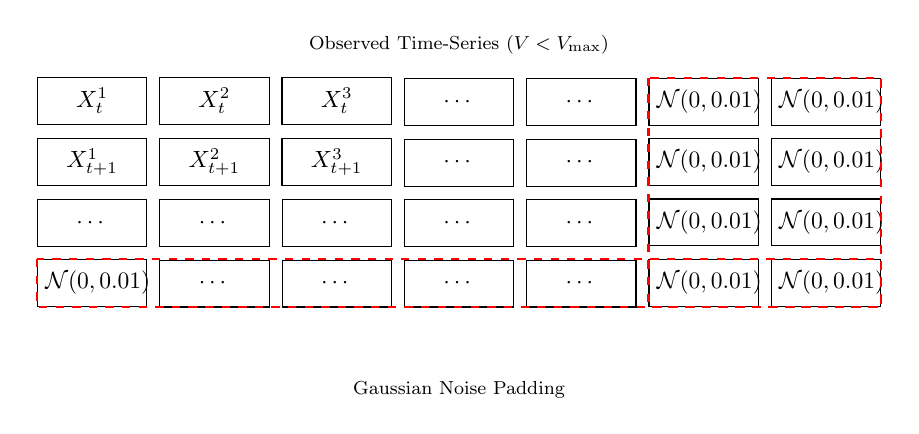
\begin{tikzpicture}[
    every node/.style={scale=0.85},
]

% Time-series matrix
\matrix (A) [matrix of nodes,
    nodes={
        draw, 
        minimum width=15mm, 
        minimum height=7mm,
        align=center,
        text width=14mm
    },
    column sep=1.5mm, row sep=1.5mm
] at (0,0)
{
  $X^1_t$ & $X^2_t$ & $X^3_t$ & $\cdots$ & $\cdots$ & $\mathcal{N}(0,0.01)$ & $\mathcal{N}(0,0.01)$ \\
  $X^1_{t+1}$ & $X^2_{t+1}$ & $X^3_{t+1}$ & $\cdots$ & $\cdots$ & $\mathcal{N}(0,0.01)$ & $\mathcal{N}(0,0.01)$ \\
  $\cdots$ & $\cdots$ & $\cdots$ & $\cdots$ & $\cdots$ & $\mathcal{N}(0,0.01)$ & $\mathcal{N}(0,0.01)$ \\
  $\mathcal{N}(0,0.01)$ & $\cdots$ & $\cdots$ & $\cdots$ & $\cdots$ & $\mathcal{N}(0,0.01)$ & $\mathcal{N}(0,0.01)$ \\
};

\node[above=2mm of A-1-4] {\footnotesize Observed Time-Series ($V < V_\text{max}$)};

% Red dashed rectangle for right padding columns
\draw[dashed, thick, red] 
    (A-1-6.north west) rectangle (A-4-7.south east);

% Red dashed rectangle for bottom padding row
\draw[dashed, thick, red] 
    (A-4-1.north west) rectangle (A-4-7.south east);

\node[below=1.6cm of A-3-4] {\footnotesize Gaussian Noise Padding};

\end{tikzpicture}
\caption{
Observed time-series matrix padded with Gaussian noise to reach \(L_\text{max}\) (sequence length) and \(V_\text{max}\) (number of variables). Red dashed boxes indicate padded regions.
}
\label{fig:input-padding-timeseries}
\end{figure}

When the number of observed time-steps (samples) \(L\) is less than the configured maximum number of samples \( L_\text{max} \), the time-series is \textit{padded with Gaussian noise \( \mathcal{N}(0,0.01)\) along the time-step dimension}. This prevents introducing zero artifacts, preserving the marginal statistics, and makes the model robust to handling varying sequence lengths. When inputs are longer than the configured maximum (either in time-steps \(L_\text{max}\) or the number of time-series \(V_\text{max}\)), the excess is \textit{truncated} to fit the maximum dimensions. This is conceptually similar to how Foundation models like the GPT family \citep{brown2020language} truncate input lengths that exceed the maximum allowed tokens. The same strategy is applied for interventional samples, illustrated in Figure \ref{fig:input-padding-timeseries}.

\subsection{Causal Graph Padding}  

\begin{figure}[h]
\centering
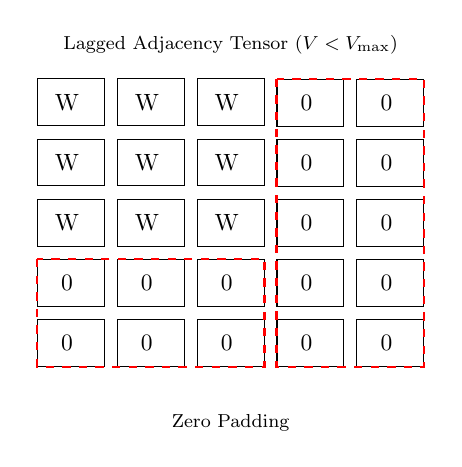
\begin{tikzpicture}[
    every node/.style={scale=0.85},
]

% Adjacency Tensor matrix
\matrix (B) [matrix of nodes,
    nodes={
        draw,
        minimum width=10mm,
        minimum height=7mm,
        align=center
    },
    column sep=1.5mm, row sep=1.5mm
] 
{
  W & W & W & 0 & 0 \\
  W & W & W & 0 & 0 \\
  W & W & W & 0 & 0 \\
  0 & 0 & 0 & 0 & 0 \\
  0 & 0 & 0 & 0 & 0 \\
};

\node[above=2mm of B-1-3] {\footnotesize Lagged Adjacency Tensor ($V < V_\text{max}$)};

% Red dashed rectangle for bottom-right padding
\draw[dashed, thick, red] 
    (B-1-4.north west) rectangle (B-5-5.south east);

% Red dashed rectangle for bottom-left padding
\draw[dashed, thick, red] 
    (B-4-1.north west) rectangle (B-5-3.south east);

\node[below=0.5cm of B-5-3] {\footnotesize Zero Padding};

\end{tikzpicture}

\caption{2D slice of a lagged adjacency tensor (e.g. lagged adjacency matrix at lag 1) padded with zeros to reach \(V_\text{max}\). Zero-padding is applied when \(V < V_\text{max}\) or \(\ell < \ell_\text{max}\). Red dashed boxes indicate padded regions.}
\label{fig:input-padding-adjtensor}
\end{figure}

A similar procedure is applied to the padding of the lagged causal graph. When a dataset comprises fewer variables than \(V < V_\text{max}\) or when the underlying causal structure assumes a lower maximum lag \(\ell < \ell_\text{max}\), the corresponding lagged adjacency tensor is \textit{zero-padded} along the unused variable and lag dimensions. This operation explicitly encodes the absence of nodes or temporal dependencies beyond the observed configuration and, together with the time-series padding described previously, constitutes a critical step for both the training and inference stages. It enables the model to uniformly process time-series and ground-truth causal graph pairs of varying time-step, node, and lag dimensionalities. During \textit{training}, the foundation model receives a time-series input—typically observational—which is propagated through the sequential blocks of the architecture to produce a lagged adjacency tensor representing the confidence of edge existence, as detailed in Section \ref{sec:problem-formulation}. The predicted tensor is subsequently compared to the appropriately padded ground-truth causal graph for loss computation, ensuring consistent alignment across lag dimensions. An illustration of the overall procedure is provided in Figure \ref{fig:input-padding-adjtensor}.


\subsection{Min--max Normalization} \label{subsec:min-max-normalization}

To ensure consistent input scaling across heterogeneous datasets and to stabilize training, all time-series variables are subjected to min--max normalization prior to being fed into the LCM, both during training and inference. This normalization step rescales each variable to the range \([0, 1]\), thereby eliminating discrepancies in magnitude that may otherwise bias learning of the internal representations toward variables with larger numerical ranges. Formally, for each variable \(x_v(t)\) in the dataset, the normalized value \(\tilde{x}_v(t)\) is computed as

\begin{equation}
\tilde{x}_v(t) = \frac{x_v(t) - \min(x_v)}{\max(x_v) - \min(x_v) + \epsilon},
\end{equation}

where \(\min(x_v)\) and \(\max(x_v)\) denote the minimum and maximum values of variable \(v\) across all timesteps, and a small constant \(\epsilon>0\) is added for numerical stability.  

This step ensures that all variables contribute comparably to the model's embedding and attention layers. During inference, i.e. with the pre-trained model weights at hand and with no ground-truth available, min--max normalization is applied using the statistics computed from the correspoding training set to maintain consistency between training and evaluation distributions.

\section{Overview of the Informer-based LCM} \label{sec:arch-informer}

In this section, we formally describe the underlying mechanisms and design of the LCM architecture, which corresponds to the Informer-based \citep{zhou2021informer} implementation of \citet{stein2024embracing}. Briefly, the building blocks revolve around an Encoder-only Transformer backbone\footnote{An introduction to the Transformer is provided in Appendix \ref{app:transformer}.}, using self-Attention instead of the Sparse Attention of the Informer, with a final feed-forward block adapted for temporal causal discovery. As the scope is not autoregressive sequence generation (i.e. in time-series forecasting or natural language processing), the model does not require a decoder block and only uses the Encoder representations to make edge predictions. Accordingly, full attention is used instead of sparse attention as the time and spaceo complexity gains of the latter are not relevant in this context.


\begin{figure}[t!]
   \centering
   \hspace*{-0.0612\textwidth}
   \includegraphics[page=1, width=1.2\textwidth]{images/figures/informer_lcm.pdf}
 \caption{Overview of the Transformer-based architecture of the LCM, following the Informer \citep{zhou2021informer} variant of \citet{stein2024embracing}. Given a multivariate time-series input of \(L\) timesteps and \(V\) variables, noise padding is performing in the timestep and variable dimensions (Section \ref{sec:input-handling}) up to \(L_{\text{max}}\) and \(V_{\text{max}}\), which are then min--max normalized (Section \ref{subsec:min-max-normalization}). Input embeddings are created using \textit{1D convolutions} and sinusoidal positional encodings. This is followed by a stack of transformer encoder blocks, performing batch normalization, multi-head self-attention and 1D convolutions, along with an \textit{optional distillation block}. Finally, a feedforward block is used to infer a lagged adjacency tensor representation and a sigmoid activation is applied to obtain edge confidence scores.}
 \label{fig:informer-architecture}
\end{figure}

Recall from Section \ref{sec:problem-formulation} that the goal of the LCM is to learn a mapping \(f_\theta\) from multivariate time-series inputs to their corresponding lagged causal adjacency graphs, by predicting a \textit{lagged adjacency tensor} \(\hat{\mathbb{A}} \in [0,1]^{V_{\max} \times V_{\max} \times \ell_{\max}}\) where each entry \(\hat{\mathbb{A}}_{ji\tau}\) denotes the probability of edge existence \(i \xrightarrow{\ell_{\max}-\tau} j\). As with any pre-trained neural architecture, we differentiate between the phases/steps:

\begin{enumerate}
  \item \textit{Training}, where the model is given as input a time-series and a ground truth causal graph pair, and outputs a lagged adjacency tensor of edge existence confidences
  \item \textit{Inference} or \textit{CD Phase}, where the model is given as input a time-series and outputs a lagged adjacency tensor \(\mathbb{\hat{A}}\) of edge existence confidences, estimating the underlying true lagged causal graph \(\mathcal{G}\) with adjacency tensor \(\mathbb{A}\).  
\end{enumerate}

The Informer-based architecture of \citet{stein2024embracing} is now described in detail, which serves as the backbone of the Large Causal Models (LCMs) and is illustrated in Figure \ref{fig:informer-architecture}.

\subsection{Input Representations} \label{sec:informer-input-reps}

In the initial input phase, the model receives an (observational) time series sample \(X \in \mathbb{R}^{B \times L \times V}\), where \(B\) denotes the \textit{batch dimension}\footnote{During causal discovery (CD) inference, the batch dimension is typically set to 1.}, \(L\) the \textit{sequence length} (number of timesteps), and \(V\) the \textit{number of variables}. Prior to any transformation, the inputs are min-max normalized. The normalized inputs are then padded along both the variable and temporal dimensions to ensure fixed dimensions \(V=V_{\max}\) and \(L=L_{\max}\), with sequences exceeding this length are truncated to \(L_{\max}\), as detailed in Section \ref{sec:input-handling}.

Each variable's time series is embedded into a higher-dimensional latent space using a 1D convolutional projection, serving as a learnable feature extractor. The convolution operates along the temporal dimension, with \(c_\text{in}=V_{\max}\) input channels and \(c_\text{out}=d_{\text{model}}\) output channels, where \(d_{\text{model}}\) denotes the \textit{model dimension}. The resulting \textit{token embeddings} are represented as

\begin{equation}
X_{\text{tok}} = \text{Conv1D}(X),
\end{equation}

yielding a tensor \(X_{\text{token}} \in \mathbb{R}^{B \times L_{\max} \times d_{\text{model}}}\). This operation captures local temporal dependencies and smooths short-range fluctuations, providing robust contextual embeddings for subsequent attention mechanisms.

Since the Transformer architecture is permutation-invariant with respect to sequence order, explicit positional information must be added to the learned embeddings. As in the vanilla Transformer by \citet{vaswani2017attention}, sinusoidal positional encodings aim to inject absolute temporal position information into the convolutional embeddings. Specifically, for each timestep \(t \in \{1, \ldots, L\}\) and embedding dimension index \(j \in \{1, \ldots, d_{\text{model}}\}\), the positional encoding is defined as:

\begin{equation}
\begin{aligned}
\mathrm{PE}_{(t, 2i)}   &= \sin\!\left(\frac{t}{10000^{2i/d_{\text{model}}}}\right), \\
\mathrm{PE}_{(t, 2i+1)} &= \cos\!\left(\frac{t}{10000^{2i/d_{\text{model}}}}\right),
\end{aligned}
\end{equation}

which are added element-wise to the learnable token embeddings:

\begin{equation}
X_{\text{emb}} = X_{\text{token}} + \mathrm{PE}.
\end{equation}

Dropout is applied to \(X_{\text{emb}}\) to improve generalization, and the resulting embeddings are reshaped and organized as \([B, L, d_{\text{model}}]\), serving as the input to the Encoder block of the Transformer.

\subsection{Transformer Encoder}

The encoded sequence \(X_{\text{emb}}\) is then processed by a stack of Informer-style Transformer encoder blocks. Each encoder blocks consists of a self-attention layer followed by a convolutional feed-forward network. Let \(E^{(l)}\) denote the input to the \(l\)-th encoder layer. Then each encoder layer computes

\begin{equation}
\begin{aligned}
E'^{(l)} &= \mathrm{LayerNorm}\big(E^{(l)} + \mathrm{SelfAttn}(E^{(l)})\big), \\
E^{(l+1)} &= \mathrm{LayerNorm}\big(E'^{(l)} + \mathrm{FFN}(E'^{(l)})\big),
\end{aligned}
\end{equation}

where \(\mathrm{SelfAttn}(\cdot)\) denotes multi-head self-attention scaled by \(1/\sqrt{d_{\text{model}}}\) as per \citet{vaswani2017attention} and \(\mathrm{FFN}(\cdot)\) represents a two-layer convolutional feed-forward block defined as

\begin{equation}
\mathrm{FFN}(x) = \mathrm{Conv1D}_2\!\left( \mathrm{GELU}\!\big(\mathrm{Conv1D}_1(x)\big) \right),
\end{equation}

applied independently at each temporal position. This convolutional replacement of the standard linear MLP (as introduced in the Informer model) allows for localized feature extraction and temporal smoothing, aiming to improve efficiency on long sequences. Each encoder block uses residual connections \citep{he2016deep} and layer normalization \citep{ba2016layer, xiong2020layer} after both the attention and feed-forward sublayers, ensuring stable gradient propagation across stacked layers.

Between successive encoder blocks, an optional \textit{self-attention distillation layer} is optionally inserted to reduce the temporal resolution, as proposed in the Informer model. In this work, distillation layer is included in all trained models. Specifically, a convolutional downsampling followed by normalization and activation is applied:

\begin{equation}
X_{\text{distil}} = \mathrm{MaxPool}\!\left( \mathrm{ELU}\!\big( \mathrm{BatchNorm}\!\big( \mathrm{Conv1D}(E^{(l)}) \big) \big) \right)
\end{equation}

which halves the temporal dimension and improves computational efficiency. Let \(E_{\text{enc}} \in \mathbb{R}^{B \times L' \times d_{\text{model}}}\) denote the encoder output after the final block, where \(L' < L\) if temporal distillation is applied. Importantly, only the final timestep embedding is retained for causal prediction, \(h = E_{\text{enc}}[:, -1, :] \in \mathbb{R}^{B \times d_{\text{model}}}\).

\subsection{Correlation Injection} \label{subsec:ci}

In an attempt to further assist the model in inferring directed dependencies, \citet{stein2024embracing} introduce a technique to inject prior statistical measures into the model, to improve performance and avoid inferring spurious relationships, as a form of \textit{training aids}. These statistical measures take the form of lagged cross-correlations between variables. For each pair \((X^i, X^j)\) and lag \(\tau \in \{1, \ldots, \ell_{\max}\}\), the empirical Pearson cross-correlation is computed as

\begin{equation}
\rho_{X^i, X^j}(\tau) = \frac{\mathrm{Cov}(X^i_{1:T-\tau}, X^j_{\tau+1:T})}{\sqrt{\mathrm{Var}(X^i_{1:T-\tau}) \, \mathrm{Var}(X^j_{\tau+1:T})}}
\end{equation}

The resulting tensor of correlations \(\mathbb{C} \in \mathbb{R}^{B \times V_{\max} \times V_{\max} \times \ell_{\max}}\) is flattened to \(\mathbb{R}^{B \times (V_{\max}^2 \cdot \ell_{\max})}\) and concatenated to the encoder representation (as shown in Figure \ref{fig:informer-architecture}):

\begin{equation}
h' = \mathrm{Concat}(h, \mathrm{Flatten}(\mathbb{C})) \in \mathbb{R}^{B \times (d_{\text{model}} + V_{\max}^2 \cdot \ell_{\max})}
\end{equation}

In Chapter \ref{chap:results}, we thoroughly evaluate the effect of correlation injection features on the performance of LCMs, filling a gap that was previously unexplored in the literature, although the authors report that this approach is effective.

\subsection{Feedforward Prediction Head}

The concatenated representation \(h'\) is then processed by a two-layer feed-forward prediction head to map latent representations to \textit{lagged adjacency predictions}. Formally,

\begin{equation}
\begin{aligned}
h_1 &= \mathrm{ELU}\!\left( \mathrm{BatchNorm}\!\left( \mathrm{Linear}_1(h') \right) \right), \\
h_2 &= \mathrm{Linear}_2(h_1),
\end{aligned}
\end{equation}

where \(\mathrm{Linear}_1 : \mathbb{R}^{d_{\text{in}}} \rightarrow \mathbb{R}^{d_{\text{ff}}}\) and \(\mathrm{Linear}_2: \mathbb{R}^{d_{\text{ff}}} \rightarrow \mathbb{R}^{V_{\max}^2 \cdot \ell_{\max}}\). The output is reshaped to form the predicted lagged adjacency tensor

\begin{equation}
\hat{\mathbb{A}} \;=\; \sigma\left( \mathrm{Reshape}\!\big(h_2\big) \right) \in [0,1]^{V_{\max} \times V_{\max} \times \ell_{\max}}
\end{equation}

where \(\sigma(x) = (1 + e^{-x})^{-1}\) is the sigmoid transformation and each element \(\hat{\mathbb{A}}_{ji\tau}\) represents the confidence of the model that a directed edge \(X^i_{t-\tau} \rightarrow X^j_t\) exists. The final sigmoid activation converts logits into interpretable probabilities of causal edge existence.

The cautious reader should notice that instead of a softmax to convert the final logits into probabilities (as in the vanilla transformer), a sigmoid is used. A sigmoid is appropriate for \textit{binary} or \textit{multi-label classification} problems where each output can be viewed as an independent Bernoulli event, while softmax is appropriate for multi-class classification where only one class is active at a time.

%%%%%%%%%%%%%%%%%%%%%%%%%%%%%%%%%%%%%%%%%%%%%%%%%%%%%%%%%%%%%%%%%%%%%%%%
%%%%%%%%%%%%%%%%%%%%%%%%%%%%%%%%%%%%%%%%%%%%%%%%%%%%%%%%%%%%%%%%%%%%%%%%

\section{Towards a novel LCM architecture} \label{sec:novel-architecture}

The aim of this section is to propose a new neural architecture for temporal causal discovery, as a successor to the Informer-based LCM model introduced earlier. Our scope is to develop an expressive model that better captures both temporal and inter-variable dependencies based on novel advances in the state-of-the-art of neural networks, while also integrating auxiliary signals such as lagged crosscorrelations described previously.


\begin{figure}[ht!]
   \centering
   \hspace*{-0.0612\textwidth}
   \includegraphics[page=1, width=1.2\textwidth]{images/figures/patchtstspacetime_lcm.pdf}
 \caption{Overview of a novel architecture for temporal causal discovery. Each time-series is split into patches, which are then projected using linear embeddings \textit{(Patch Embeddings)}. Standard sinusoidal positional encodings are added, together with variable embeddings (for carrying variable identity information) and passed through a stack of transformer encoder blocks, consisting of Temporal \& Spatial multi-head attention. The resulted outputs are concatenated with crosscorrelation statistical measures \textit{(training aids)} as a way to further increase the expressiveness of the model. They are finally processed through a feedforward head and a sigmoid activation to predict a lagged adjacency tensor \(\hat{\mathbb{A}} \in \mathbb{R}^{V_{\max} \times V_{\max} \times \ell_{\max}}\) that represents the discovered lagged causal graph.}
 \label{fig:lcm_novel-architecture}
\end{figure}

An overview of the proposed model is shown in Figure \ref{fig:lcm_novel-architecture}. Conceptually, the design follows four sequential stages, as in the Informer-based LCM: (i) \textit{Input preprocessing and patch embeddings} where the multivariate time-series is normalized, divided into overlapping temporal patches, and projected into a latent embedding space enriched with positional and variable identity information, (ii) \textit{Transformer Encoder with decoupled temporal and spatial attention}, using alternating self-attention over time and variables to jointly learn dynamic and cross-variable dependencies, (iii) \textit{auxiliary inputs} where lagged crosscorrelation is concatenated alongside the learned representations to guide causal learning and (iv) \textit{prediction head} serving as a feedforward projection using a SwiGLU \citep{shazeer2020glu} activation and a sigmoid output to yield the lagged causal adjacency tensor \(\hat{\mathbb{A}} \in [0,1]^{V_{\text{max}} \times V_{\text{max}} \times \ell_{\text{max}}}\) representing the probability of causal influence across variables and lags.

\subsection{Input representations}  \label{sec:input-representations}

As in the Informer-based LCM, the model receives an (observational) time-series sample \(X \in \mathbb{R}^{B \times L \times V}\)
where \(B\) denotes the batch size, \(L\) the sequence length (timesteps), and \(V\) the number of variables. \(X\) is min-max normalized and padded as detailed in Sections \ref{sec:input-handling} and \ref{subsec:min-max-normalization}. 

%\subsection{Patching}

Instead of processing individual timesteps directly as before, the model employs a \textit{patching mechanism} \citep{nie2023time}, transforming each variable's sequence into overlapping windows of length \(\rho\) and stride \(s\):

\begin{equation}
L' = \left\lfloor \frac{L - \rho}{s} \right\rfloor + 1
\end{equation}

Each variable's sequence is split independently, yielding an intermediate tensor representation \([B, V_{\max}, L', \rho]\) which is afterwards reshaped into an embedding representation \([B \cdot V_{\max}, L', \rho]\). This operation reduces the effective sequence length while simultaneously allowing each patch to encapsulate short-term temporal dynamics, enabling efficient modeling of long-range dependencies.

%\subsection{Patch Embeddings}

Each patch \(P \in \mathbb{R}^{\rho}\) is then projected to the model dimension \(d_\text{model}\) via a learnable linear transformation:

\begin{equation}
\hat{P} = W_P P + b_P, \quad W_P \in \mathbb{R}^{d_{\text{model}} \times \rho}
\end{equation}

where \(W_P\) and \(b_P\) are learnable parameters. To preserve temporal order across patches, \textit{sinusoidal positional encodings} \citep{vaswani2017attention} are added element-wise, as defined previously in Section \ref{sec:informer-input-reps}:

\begin{equation}
\hat{P}^{\text{pos}} = \hat{P} + \mathrm{PosEmb}(\ell)
\end{equation}

where \(\ell\) indexes the position of the patch within the sequence. Each variable is also assigned a learnable \textit{variable embedding} \(e_j \in \mathbb{R}^{d_{\text{model}}}\), shared across patches, encoding variable identity information and facilitating inter-variable disambiguation. The final embedding sequence

\begin{equation}
X_{\text{emb}} \in \mathbb{R}^{B \times L' \times V_{\max} \times d_{\text{model}}}
\end{equation}

is obtained after dropout regularization \citep{srivastava2014dropout} and reshaping, and serves as the input to the Encoder block.

\subsection{Encoder block}

The encoder consists of (N) identical blocks. Each block alternates \textit{temporal attention} (multi-head attention across patches within each variable) and \textit{spatial attention} (multi-head attention across variables within a patch). This decoupling allows the model to explicitly disentangle intra-variable temporal dynamics from inter-variable dependencies. Specifically, for each variable \(i\), temporal attention is computed as:

\begin{equation}
\text{TemporalAttn}^i = \text{MultiHeadAttn}(Q^i, K^i, V^i)
\end{equation}

resulting in \(X \in \mathbb{R}^{B \times P \times V_{\max} \times d_{\text{model}}} \). To enhance \textit{permutation equivariance across features}, a permutation-equivariant transformation \(\phi\) is introduced, followed by \textit{mean pooling} across the variable dimension:

\begin{equation}
X_{\text{agg}} = \frac{1}{V_{\text{max}}}\sum_{i=1}^{V_{\text{max}}} \phi(X_i)
\end{equation}

inspired by Deep Sets \citep{zaheer2017deep}. This global summary is added back to the temporally attended features and normalized:

\begin{equation}
X' = \text{LayerNorm}(X + X_{\text{agg}})
\end{equation}

The updated representations are then passed through \textit{spatial attention}, \textit{layer normalization} and a \textit{feedforward network}:

\begin{equation}
\text{FF}(x) = W_2 , \mathrm{GeLU}(W_1 x + b_1) + b_2
\end{equation}

each wrapped with residual connections. It should be noted that since a feedforward network is applied, no permutation equivariance is preserved, although the transformation \(\phi\), together with mean pooling aim towards a permutation-equivariant model. Finally, temporal aggregation is performed by mean-pooling across patches:

\begin{equation}
\bar{X} = \frac{1}{L'} \sum_{p=1}^{L'} X_{:,p,:,:} \in \mathbb{R}^{B \times V_{\max} \times d_{\text{model}}}
\end{equation}

Since our objective is not sequence generation, no decoder block is used (as in Section \ref{sec:arch-informer}). The encoder's output logits directly represent causal feature interactions.

\subsection{Auxiliary Inputs}

\begin{equation}
\rho_{X^i,X^j}(\tau) = \frac{\mathrm{Cov}(X^i_{1:T-\tau}, X^j_{\tau+1:T})}{\sqrt{\mathrm{Var}(X^i_{1:T-\tau}) , \mathrm{Var}(X^j_{\tau+1:T})}}
\end{equation}

for \(\tau = 1, \dots, \ell_{\max}\). These are assembled into \(\mathbb{C} \in \mathbb{R}^{B \times V_{\max} \times V_{\max} \times \ell_{\max}}\), flattened, and concatenated to the logits of the final encoder block

\begin{equation}
Z = \mathrm{Concat}(X_{\text{enc}}, \mathbb{C})
\end{equation}


\subsection{Feedforward Prediction Head}

The concatenated representation is projected through a two-layer feedforward head with layer normalization and \textit{SwiGLU activation} \citep{shazeer2020glu}, followed by a sigmoid transformation:

\begin{equation}
\hat{\mathbb{A}} = \sigma\left(\text{reshape}\left(W_2 \cdot \text{SwiGLU}\big(\text{LN}(W_1 Z + b_1)\big) + b_2 \in [0,1]^{B \times V_{\max} \times V_{\max} \times \ell_{\max}} \right)\right)
\end{equation}

where the SwiGLU activation is defined as

\begin{equation}
  \text{SwiGLU}(x) = (xW_1) \odot \text{SiLU}(xW_2),
\end{equation}

where \(W_1\) and \(W_2\) are learned projection matrices, and \(\odot\) denotes elementwise multiplication. The function \(\text{SiLU}(z) = z \cdot \sigma(z)\) denotes the \textit{Sigmoid Linear Unit} (also known as the \textit{Swish} activation), which combines linear gating with smooth nonlinear modulation, leading to improved gradient flow and expressivity compared to standard activations such as ReLU or GELU. 

The output tensor \(\hat{\mathbb{A}}\) is interpeted in the same manner as in the Informer-based model in Section \ref{sec:arch-informer}.

\section{Expanding the Scope of LCMs} \label{sec:scope-expansion}

This section explores two complementary extensions for causal foundation models, the incorporation of \textit{interventional samples} and \textit{prior knowledge}, in Subsection \ref{subsec:scope-interventions} and Subsection \ref{subsec:scope-prior}, respectively.

\subsection{Towards Incorporating Interventional Samples} \label{subsec:scope-interventions}

A central motivation in causal discovery is to move beyond mere association and towards identifiability of the underlying causal graph. While observational data allow the estimation of correlations and potential dependencies, they are insufficient to fully resolve causal directions in many cases due to the problem of statistical indistinguishability among Markov-equivalent structures. As an example in the i.i.d. setting, two variables \(X\) and \(Y\) may be highly correlated, yet share an unobserved common cause. If a CD algorithm assumes causal sufficiency (Section \ref{sec:setting} \& Table \ref{tab:causal-assumptions}), then an edge from \(X\) to \(Y\) will be identified. To overcome this limitation, interventional data play a critical role: by intervening on \(X\) and observing \(Y\), it is becomes possible to resolve the causal direction. Practical examples include controlled modifications in software configuration parameters for AIOps, targeted marketing campaigns in economics or knockout experiments in biological networks. By explicitly introducing interventions in the model, the model is provided with more informative samples that aims to improve causal identifiability.

To accomplish this, we accompany each input batch with a \textit{binary interventional matrix} \(B_{K \times V} \in {0, 1}\) such that 

\begin{equation}
B_{ij} =
\begin{cases}
1, & \text{if variable } V_j \text{ was directly intervened at timestep } i, \\
0, & \text{if } V_j ~\text{remained observational at timestep } i
\end{cases}
\end{equation}

where \(K\) denotes the number of interventional time-steps and \(V\) the number of variables. Thus, \(B_{ij} = 1\) can be interpreted as a \textit{masking operation}, indicating that the corresponding observation no longer reflects the natural dependency structure, as the variable's causal parents have been disrupted by an external intervention. As in the observational inputs, the interventional samples are padded as per Section \ref{sec:input-handling}, while the interventional matrix is padded with zeros where needed, to match the maximum number of time-steps \(K_\text{max}=L_\text{max}\) and variables \(V_\text{max}\).

\begin{figure}[h!]
   \centering
   \hspace*{-0.0612\textwidth}
   \includegraphics[page=1, width=1.2\textwidth]{images/figures/interv-integration.pdf}
   \vspace{-10pt}
   \caption{Integration of interventional samples in an LCM. Each input time series is accompanied by a binary interventional mask \(B\), which encodes which variables were externally manipulated. The mask is concatenated with the encoder outputs, allowing the model to condition the following prediction layers based on the context of interventions.}
 \label{fig:interv-integration}
\end{figure}

During both training and inference, the (padded) binary interventional mask \(B_{K_\text{max} \times V_\text{max}}\), together with interventional samples are concatenated with the encoded latent representation of the input time series (Figure \ref{fig:interv-integration}). Formally, for a given encoder output \(\mathbf{H}\), the augmented representation becomes 

\begin{equation}
\mathbf{H'} = \text{Concat}(\mathbf{H}, B)
\end{equation}

where \(B\) is broadcast or flattened to match the structure of \(\mathbf{H}\). This augmentation allows the downstream attention and prediction layers to explicitly condition on which variables were intervened upon, thereby guiding the network to adjust its learned dependencies accordingly. 

In essence, the model already learns, up to the final encoder block, to identify causal relationships. From there, the augmentation of the output is fed into the feedforward prediction head, which aims to further refine the prediction of the true causal directions by differentiating between observational and interventional examples. Over many such interventional samples, the model learn to internalize which dependencies are consistent under both observational and interventional conditions, yielding more accurate and identifiable causal graphs. The combination of interventional and observational data thus aims to extend the scope of neural foundation models beyond observational data alone.


\subsection{Towards Incorporating Prior Knowledge} \label{subsec:scope-prior}

In many real-world domains, partial knowledge of causal relationships is often available or can be constructed manually by experts. This information can come in the form of known causal edges or paths (i.e. (“\(A\) causes \(B\)”)) or exclusions (“\(A\) does not cause \(B\)”), and may include varying degrees of confidence. Incorporating such domain knowledge into a neural causal discovery model can improve interpretability and robustness, especially under limited data or noisy observational settings. However, unlike constraint-based algorithms such as PCMCI \citep{runge2018causal} which can directly encode hard constraints, neural architectures exhibit intrinsic stochasticity and non-linearity that make strict enforcement of such constraints impractical. 

To incorporate domain information into the model, prior knowledge is injected after the last encoder block (in a similar manner to correlation injection and handling of interventions), allowing the model to refine its learned representations to more plausible causal structures without constraining it from the beginning. Prior information is provided either in edges and paths (edges are a special case of paths with length 1). By path, we mean a sequence of edges in the lagged causal graph of the form \( X^{i}_{t-2} \rightarrow X^{j}_{t-1} \rightarrow X^{k}_{t}\) where \(t \in \mathbb{N}\). The assumption of causal stationarity also applies to paths, making them time-invariant.

\begin{figure}[t!]
  \centering
  \hspace*{-0.0612\textwidth}
  \includegraphics[page=1, width=1.2\textwidth]{images/figures/prior-integration.pdf}
  \caption{Integration of prior knowledge in an LCM. Prior tensors \(\mathcal{P}\) and belief masks \(\mathcal{B}\) are flattened and concatenated with the encoder output, aiming to provide soft inductive biases toward known or excluded edges and paths. This enables the model to learn causal structures that are consistent with provided knowledge while remaining data-adaptive.}
  \label{fig:prior-integration}
\end{figure}

Specifically, information about priors is represented by two tensors: (i) a \textit{prior tensor} \(\mathcal{P} \in \left\{0,1,2\right\}^{V_{\max} \times V_{\max} \times \ell_{\max}}\) and (ii) a \textit{belief strength mask} \(\mathcal{B} \in [0,1]^{V_{\max} \times V_{\max} \times \ell_{\max}}\), associating each entry of \(\mathcal{P}\) with a strength of knowledge for each edge/path. Both \(\mathcal{P}\) and \(\mathcal{B}\) share the same semantics as the adjacency tensor representation in Section \ref{sec:problem-formulation}. Information in \(\mathcal{P}\) is encoded as follows:

\begin{equation}
\mathcal{P}_{ji\ell} =
\begin{cases}
0, & \text{no prior knowledge available},\\
1, & \text{if edge/path \(X^i_{t-\ell} \rightarrow X^j_t\) is known to exist - inclusion prior},\\
2, & \text{if edge/path \(X^i_{t-\ell} \rightarrow X^j_t\) is known to not exist - exclusion prior}
\end{cases}
\end{equation}

where the above formulation possesses the same semantics as our the adjacency tensor representation of the causal graph and accounts for paths up to \(\ell_{\max}\).

The prior information is flattened and concatenated with the output of the final encoder block, similarly to the case of interventions, as illustrated in Figure \ref{fig:prior-integration}. As it should be clear so far to the cautious reader, these two auxiliary prior inputs are provided during both inference and training, following a methodology described in Section \ref{sec:training-prior} of Chapter \ref{chap:training}.
	%\chapter{Training} \label{chap:training}

\begin{chapquote}{\textit{John Tukey}}
``Far better an approximate answer to the right question, which is often vague, than an exact answer to the wrong question, which can always be made precise.''
\end{chapquote}

This chapter provides a detailed treatment of the training process of our LCMs. It serves as an extension of our high-level discussion in Section \ref{sec:dl}, but tailored specifically towards the training of our LCMs. We begin by outlining the basic components of our training process and the associated challenges, before moving on to the main objectives of our work.

\section{Optimization Strategies \& Optimizers} \label{sec:optimizer}

As briefly mentioned in Section \ref{sec:dl}, a neural network model attempts to solve an optimization problem. Broadly speaking, this concerns finding the best possible values of its trainable parameters, over all feasible ones. The optimization problem is typically formulated as a \textit{minimization problem}, where the goal is to find the set of parameters that minimizes a loss function. For a regression task, this means minimizing the expectation of the loss function over the parameters \(\theta\) of a trainable neural model \(f_\theta\), where the expectation is taken with respect to the underlying joint distribution \(p_{X,Y}\) that our input-output training data is assumed to follow. Mathematically, this corresponds to

\begin{equation}
\theta^{*} = \text{argmin}_{\theta \in \Theta} \mathbb{E}_{(X,Y) \sim p_{X,Y}} \left[\mathcal{L}(f(x;\theta), Y)\right]
\end{equation}
 
where \(x\) is the input (in our case, the time-series samples) and \(y\) the corresponding label (the ground truth lagged adjacency tensor from the ground truth TSCM), \(\Theta\) the parameter space, \(\theta\) the optimal parameter set and \(\mathcal{L}\) the loss function. Once the expectation is computed, all variables become fixed except for the parameters \(\theta\) of the model. In this sense, only those are left to determine the functions value, which corresponds to the minimization of our quantity of interest. As may be already evident, this problem is \textit{intractable} and is solved by an algorithm that dictates how and when the parameters \(\theta\) are updated over time during training, such that convergence as close as possible to the true minimum is achieved. This role is assigned to the \textit{optimizer} that is used, which is a rigid part of the training protocol.

There are many optimizers to choose from depending on the implemented architecture and nature of the problem. It may even be the case that only one carefully tuned optimizer can adequately train the weights of a specific network. Nonetheless, some optimizers have proven to work well in most circumstances. A treatment of the most common ones is provided in Appendix \ref{app:optimizers}.

\begin{algorithm}[t]
\caption{AdamW Optimizer} \label{alg:adamw}
\begin{algorithmic}[1]
\renewcommand{\algorithmicrequire}{\textbf{Input:}}
\renewcommand{\algorithmicensure}{\textbf{Output:}}
\REQUIRE Parameters $\theta$, learning rate $\eta$, $\beta_1, \beta_2 \in [0,1)$, weight decay $\lambda$, $\epsilon > 0$
\ENSURE Updated parameters $\theta$
\STATE Initialize $m_0 \gets 0$, $v_0 \gets 0$, $t \gets 0$
\FOR{each iteration}
    \STATE $t \gets t+1$
    \STATE Sample mini-batch and compute gradient $g_t \gets \nabla_\theta \mathcal{L}(\theta)$
    \STATE $m_t \gets \beta_1 m_{t-1} + (1 - \beta_1) g_t$
    \STATE $v_t \gets \beta_2 v_{t-1} + (1 - \beta_2) g_t^2$
    \STATE $\hat{m}_t \gets \frac{m_t}{1 - \beta_1^t}$
    \STATE $\hat{v}_t \gets \frac{v_t}{1 - \beta_2^t}$
    \STATE $\theta \gets \theta - \eta \cdot \left(\frac{\hat{m}_t}{\sqrt{\hat{v}_t} + \epsilon} + \lambda \theta\right)$
\ENDFOR
\end{algorithmic}
\end{algorithm}

For training our LCMs, we use the Adam optimizer \citep{loshchilov2017fixing} which serves as a popular extension of Adam \citep{kingma2015adam}. AdamW was introduced to fix a subtle but important flaw in Adam regarding weight decay (commonly used for regularization). In classical Adam, weight decay is typically implemented by adding an \(L_2\) penalty term to the loss function. However, this approach causes the penalty to interact with Adam's adaptive learning rate mechanism in unintuitive ways: instead of applying a simple shrinkage to the parameters, the effective weight decay is scaled differently for each parameter depending on its learning rate. This leads to inconsistent and sometimes poor generalization performance. AdamW resolves this by decoupling weight decay from the gradient update rule. In practice, this means that the weight decay term is applied directly to the parameter update rule (line 9 in Algorithm \ref{alg:adamw}), independently of the adaptive gradient correction. The effect is a more consistent and theoretically justified form of regularization. Empirically, AdamW has been shown to improve generalization, especially in large-scale deep learning models such as Transformers and convolutional networks, and it is now the optimizer of choice in many modern architectures, such as in BERT \citep{devlin2019bert}. 

\section{Loss Functions} \label{sec:loss-functions}

Since a neural network must learn the mapping from inputs to desired outputs, a fundamental requirement is a mechanism to quantify how “close” or “far” the network's predictions are from the ground truth. The loss function serves precisely this role—its magnitude measures the discrepancy between the model's estimates and the target causal structure. The optimization objective is therefore to minimize this loss across all training examples.

\subsection{Binary Cross-Entropy Loss} \label{subsec:bce}

For our LCMs, each possible directed edge \(V^i_{t-\ell} \rightarrow V^j_t\) in the lagged causal graph corresponds to a Bernoulli random variable encoding the presence or absence of a direct causal relationship. As elaborated in Section \ref{sec:problem-formulation}, predicting causal edges naturally takes the form of a binary classification task, where the model outputs a confidence score \(\hat{\mathbb{A}}_{ji\ell} \in [0,1]\) representing the estimated probability that a direct lagged edge \(V^i_{t-\ell} \rightarrow V^j_t\) exists.

Let \(a_i \in {0,1}\) denote the ground-truth label for the \(i\)-th edge and \(\hat{a}_i \in [0,1]\) the model's predicted probability. The likelihood of the observed labels given the predictions can be modeled as a product of independent Bernoulli variables:

\begin{equation}
p(\mathbf{a} \mid \mathbf{\hat{a}}) = \prod_{i=1}^{N} \hat{a}_i^{a_i} (1 - \hat{a}_i)^{1 - a_i}
\end{equation}

where \(N = V_{\max}^2 \times \ell_{\max}\) is the total number of potential lagged edges. Maximizing this likelihood is equivalent to minimizing the \textit{negative log-likelihood (NLL)}:

\begin{equation}
\mathcal{L}_{\text{BCE}}(\mathbf{a}, \mathbf{\hat{a}})
= -\frac{1}{N} \sum_{i=1}^{N} \left[ a_i \log(\hat{a}_i) + (1 - a_i) \log(1 - \hat{a}_i) \right]
\label{eq:bce-basic}
\end{equation}

This defines the \textit{Binary Cross-Entropy (BCE)} loss, a standard choice for supervised binary prediction tasks. It penalizes incorrect predictions more heavily when the model is confident but wrong, owing to the logarithmic growth of the loss as \(\hat{a}_i \to 0\) for positive labels (\(a_i = 1\)) or \(\hat{a}_i \to 1\) for negative labels (\(a_i = 0\)).

The model produces logits \(z_i \in \mathbb{R}\), which are converted to probabilities via the sigmoid function \(\hat{a}_i = \sigma(z_i) = (1 + e^{-z_i})^{-1}\). Substituting this into Equation \ref{eq:bce-basic} yields the BCE loss in terms of logits:

\begin{equation}
\mathcal{L}_{\text{BCEWithLogits}}(\mathbf{a}, \mathbf{z})
= -\frac{1}{N} \sum_{i=1}^{N} \left[a_i \log \sigma(z_i) + (1 - a_i) \log (1 - \sigma(z_i))\right]
\label{eq:bce-logits}
\end{equation}

For numerical stability, training employs the fused \texttt{BCEWithLogitsLoss} formulation, which combines the sigmoid activation and BCE computation into a single operation to prevent overflow and ensure stable gradients. Differentiating with respect to \(z_i\) gives:

\begin{equation}
\frac{\partial \mathcal{L}_{\text{BCE}}}{\partial z_i} = \sigma(z_i) - a_i = \hat{a}_i - a_i
\end{equation}

showing that the gradient corresponds directly to the difference between predicted and true probabilities. Denoting \(\hat{\mathbb{A}}\) and \(\mathbb{A}\) as the predicted and true lagged adjacency tensors, respectively, the BCE loss over a mini-batch is computed as:

\begin{equation}
\mathcal{L}_{\text{BCE}}(\mathbb{A}, \hat{\mathbb{A}}) = -\frac{1}{V^2_{\max} \cdot \ell_{\max}}
\sum_{i,j=1}^{V_{\max}} \sum_{\ell=1}^{\ell_{\max}}
\left[
A_{ij}^{(\ell)} \log \hat{\mathbb{A}}_{ji \ell} + (1 - \mathbb{A}_{ji\ell}) \log (1-\hat{\mathbb{A}}_{ji\ell})
\right]
\label{eq:bce-lcm}
\end{equation}

\subsection{Correlation Regularization} \label{subsec:cr}

In addition to the primary BCE loss, we introduce a correlation-based regularization term designed to guide the model toward statistically plausible edge predictions. The intuition is to incorporate observable signal-level dependencies as auxiliary information, a form of \textit{training aid}, to encourage the model to assign high causal confidence only where empirical evidence supports it.

This \textit{Correlation Regularization} (CR) term penalizes predicted edges between variable pairs whose empirical lagged cross-correlation is low. Following the formulation introduced by \citet{stein2024embracing}, we define:

\begin{equation}
\mathcal{L}_{\text{CR}}(\hat{\mathbb{A}}, X) = \sum_{i,j=1}^{V_{\max}} \sum_{\ell=1}^{\ell_{\max}}
\frac{\hat{\mathbb{A}}_{ji\ell}}{\left(|\mathrm{CC}(X_j, X_i, \ell)| + \epsilon\right)^{3/2}}
\end{equation}

where \(\mathrm{CC}(X_j, X_i, \ell)\) denotes the empirical lagged cross-correlation between variables \(X_j\) and \(X_i\) at lag \(\ell\), computed over the observed time-series segment, and \(\epsilon = 10^{-6}\) ensures numerical stability. The exponent \(3/2\) accentuates the penalty for near-zero correlations while preserving smooth gradients for moderately correlated pairs. In implementation, both the ground truth \(\mathbb{A}\) and the predicted tensor \(\hat{\mathbb{A}}\) are flattened to one-dimensional tensors of length \(V_{\max}^2 \times \ell_{\max}\) before computing the BCE loss. The total loss used for training LCMs thus becomes:

\begin{equation}
\mathcal{L} = \mathcal{L}_{\text{BCE}} + \lambda_{\text{CR}} \cdot \mathcal{L}_{\text{CR}},
\end{equation}

where \(\lambda_{\text{CR}}\) is a tunable hyperparameter controlling the strength of the correlation-based penalty. In practice, this term discourages spurious edge predictions and promotes generalization by anchoring causal inference to observable statistical structure. Extensive ablation experiments are performed in Chapter \ref{chap:results} to quantify its effect on model stability and performance.


\section{Training Protocol and Data Splits} \label{sec:training-prot}

All models are trained on the curated datasets described in Chapter \ref{chap:data}. Each dataset follows an 80/10/10\% split into training, validation, and test subsets to ensure a fair evaluation and prevent data leakage. Mini-batches are randomly sampled from the training set and optimization is performed using the AdamW optimizer (Section \ref{sec:optimizer}) with default parameters \(\beta_1 = 0.9\), \(\beta_2 = 0.999\) for a maximum of \(100\) epochs.


\section{Training Challenges \& Practical Remedies}

This section covers techniques in the optimizer and training protocol that help overcome challenges encountered when training not only our LCMs but deep neural architectures in general. As models become larger and datasets more complex, effective training is impeded by issues such as limited computational resources, data quality and quantity constraints, optimization difficulties like vanishing gradients, training instability, and overfitting. Remedies including advanced optimizer designs, learning rate scheduling, gradient accumulation, regularization, and adaptive training strategies enable more efficient and stable learning. By understanding and addressing these challenges with appropriate methods, it becomes possible to train larger, more accurate models that generalize well to unseen data.


\subsection{Gradient Accumulation}

\begin{figure}[t!]
    \centering
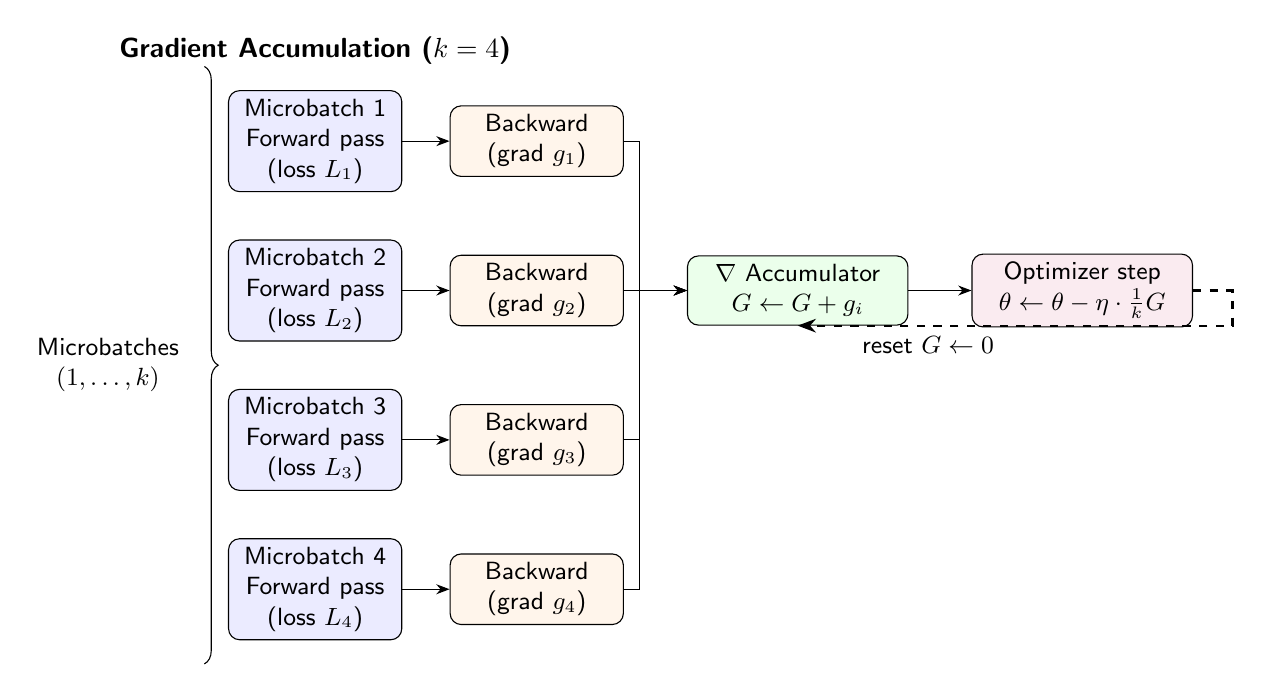
\begin{tikzpicture}[
  node distance=6mm and 6mm, 
  >=Stealth, 
  every node/.style={font=\sffamily\small}, 
  box/.style={draw,rounded corners,inner sep=3pt,minimum width=22mm,align=center},
  fwd/.style={box,fill=blue!8},
  bwd/.style={box,fill=orange!8},
  acc/.style={box,fill=green!8},
  opt/.style={box,fill=purple!8}
]

% Microbatches
\node[fwd] (F1) {Microbatch 1\\Forward pass\\(loss $L_1$)};
\node[bwd, right=of F1] (B1) {Backward\\(grad $g_1$)};
\draw[->] (F1) -- (B1);

\node[fwd, below=of F1] (F2) {Microbatch 2\\Forward pass\\(loss $L_2$)};
\node[bwd, right=of F2] (B2) {Backward\\(grad $g_2$)};
\draw[->] (F2) -- (B2);

\node[fwd, below=of F2] (F3) {Microbatch 3\\Forward pass\\(loss $L_3$)};
\node[bwd, right=of F3] (B3) {Backward\\(grad $g_3$)};
\draw[->] (F3) -- (B3);

\node[fwd, below=of F3] (F4) {Microbatch 4\\Forward pass\\(loss $L_4$)};
\node[bwd, right=of F4] (B4) {Backward\\(grad $g_4$)};
\draw[->] (F4) -- (B4);

% Grad ccumulator box
\node[acc, right=8mm of B2, minimum width=28mm] (ACC) {\(\nabla\) Accumulator\\$G \gets G + g_i$};

\foreach \X in {B1,B2,B3,B4} {
  \draw[->] (\X.east) -- ++(2mm,0) |- (ACC.west);
}

% Optimizer box 
\node[opt, right=8mm of ACC, minimum width=28mm] (OPT) {Optimizer step\\$\theta \gets \theta - \eta \cdot \tfrac{1}{k} G$};
\draw[->] (ACC.east) -- (OPT.west);

% Reset arrow
\draw[->, dashed, thick] (OPT.east) -- ++(5mm,0) |- (ACC.south)
  %node[pos=0.35,right,align=left] {\small reset $G \leftarrow 0$};
  node[pos=0.85,below,align=center] {reset $G \leftarrow 0$};

% Header
\node[above=2mm of F1, font=\sffamily\bfseries] {Gradient Accumulation ($k=4$)};

% Brace
\draw[decorate,decoration={brace,amplitude=5pt}] 
  ($(F1.north west)+(-3mm,3mm)$) -- ($(F4.south west)+(-3mm,-3mm)$) 
  node[midway,left=2mm,align=center] {Microbatches\\$(1,\ldots,k)$};

\end{tikzpicture}
\caption{Illustration of the gradient accumulation method \citep{huang2019gpipe}. Instead of performing a parameter update after a single batch, gradients from multiple forward and backward passes of smaller batches (microbatches) are sequentially accumulated in a dedicated buffer (the \textit{gradient accumulator}). After \(k\) microbatches, the aggregated gradient (summed or averaged) is applied in a single optimizer step to update the model parameters, followed by a reset of the accumulator. This approach allows training with effectively larger batch sizes while reducing memory usage, since only one microbatch needs to reside in memory at a time.}
\label{fig:grad-accumulation}
\end{figure}

As deep neural networks become larger on the number of parameters, an important issue is training under memory constraints. For the most part, training deep neural architectures require large amounts of memory resources for storing model parameters and their gradients, even for just fine-tuning of pre-trained large scale models. A significant question is thus how to allow efficient training when memory resources are limited. In literature, primarily two memory reduction methods have been introduced to tackle the aforementioned problem: \textit{gradient accumulation} \citep{huang2019gpipe} and \textit{gradient release} \citep{pudipeddi2020training}.

Gradient accumulation allows us to simulate training with a larger \textit{effective batch size} by reducing the activation memory. As illustrated in Figure \ref{fig:grad-accumulation}, instead of updating parameters after every mini-batch, we compute gradients for several small mini-batches (\textit{microbatches}), accumulate them in memory and only apply the optimizer update once after \(k\) steps (selecting \(k=4\) for large models). This means the effective batch size = (mini-batch size) \(\times\) (accumulation steps). Gradient accumulation allows training of large-scale LCMs by simulating larger batch sizes when memory limitations prevent larger batch sizes. This is crucial since each batch may consist of hundreds of multivariate time-series samples with long temporal horizons. By accumulating gradients over \(k=4\) steps before applying an update, we approximate the stability of training with a larger batch (known as the \textit{effective batch size}). Algorithm \ref{alg:grad-accumulation} describes the gradient accumulation method.

This approach has been experimentally shown to have no negative impact on training and convergence, although a small trade-off exists: In a sense, small batches can be noisy and thus lead to some training instability, or have a regularizing effect and lead to a better global minimum, while larger batches can be more stable but generalize less well.

In all training experiments, we utilize an \textit{effective batch size of \(B=64\)}. We thus select \(k=4\) when gradient accumulation is used for large-scale models (\( > 10M\) parameters) to simulate an effective batch size of \(B\).  

\begin{algorithm}[ht!]
\caption{Gradient Accumulation} \label{alg:grad-accumulation}
\begin{algorithmic}[1]
\renewcommand{\algorithmicrequire}{\textbf{Input:}}
\renewcommand{\algorithmicensure}{\textbf{Output:}}
\REQUIRE Accumulation steps $k$, optimizer, model $f_\theta$, dataset $\mathcal{D}$
\ENSURE Updated parameters $\theta$
\STATE $step \gets 0$
\FOR{each epoch}
    \FOR{microbatch $B \subseteq \mathcal{D}$}
        \STATE Compute loss $L_B \gets \mathcal{L}(f_\theta(B))$
        \STATE Compute gradients $g_B \gets \nabla_\theta L_B$
        \STATE Accumulate gradients: $G \gets G + g_B$
        \STATE $step \gets step + 1$
        \IF{$step \bmod k = 0$}
            \STATE Update parameters: $\theta \gets \theta - \eta \cdot G$
            \STATE Reset accumulator $G \gets 0$
        \ENDIF
    \ENDFOR
\ENDFOR
\end{algorithmic}
\end{algorithm}


\subsection{Early Stopping}

Early stopping (Algorithm \ref{alg:early-stopping}) is a fundamental regularization technique when training of machine learning models. The main objective is to prevent overfitting (i.e. the model learns the training data's noise and idiosyncrasies rather than its underlying patterns) by monitoring the validation loss over epochs. The algorithm uses two key hyperparameters to achieve this goal: (i) the \textit{minimum improvement threshold} \(\delta\), which is a small margin designed to prevent the algorithm from terminating prematurely due to minor, non-significant fluctuations in the validation loss and (ii) the \textit{patience term} \(\rho\) which specifies the number of epochs to wait for a significant improvement in the validation loss before stopping. We adopt a patience value of \(\rho=20\) to accommodate the often slow and fluctuating convergence patterns observed in the training of deep neural networks, allowing the model to adapt through periods of stagnated improvement without premature termination.

\begin{algorithm}[t!]
\caption{Early Stopping for LCM Training} \label{alg:early-stopping}
\begin{algorithmic}[1]
\renewcommand{\algorithmicrequire}{\textbf{Input:}}
\renewcommand{\algorithmicensure}{\textbf{Output:}}
\REQUIRE Validation loss sequence $\{val\_loss^{(e)}\}$, patience $p$, minimum improvement $\delta$
\ENSURE Best epoch $e^*$ or stop signal

\STATE $best\_val\_loss \gets \infty$
\STATE $counter \gets 0$
\FOR{epoch $e = 1, 2, \dots$}
    \STATE Compute $val\_loss^{(e)}$
    \IF{$val\_loss^{(e)} < best\_val\_loss - \delta$}
        \STATE $best\_val\_loss \gets val\_loss^{(e)}$
        \STATE $e^* \gets e$
        \STATE $counter \gets 0$
    \ELSE
        \STATE $counter \gets counter + 1$
    \ENDIF
    \IF{$counter \geq p$}
        \STATE \textbf{stop training} and return $e^*$
    \ENDIF
\ENDFOR
\end{algorithmic}
\end{algorithm}

\subsection{Learning Rate Scheduler}

\begin{algorithm}[h]
\caption{Learning Rate Scheduler for LCM Training} \label{alg:scheduler}
\begin{algorithmic}[1]
\renewcommand{\algorithmicrequire}{\textbf{Input:}}
\renewcommand{\algorithmicensure}{\textbf{Output:}}
\REQUIRE Initial learning rate $\eta$, reduction factor $\gamma < 1$, patience $p_{lr}$, min\_lr
\ENSURE Adaptively updated $\eta$
\STATE $best\_val\_loss \gets \infty$
\STATE $counter \gets 0$
\FOR{epoch $e = 1, 2, \dots$}
    \STATE Compute $val\_loss^{(e)}$
    \IF{$val\_loss^{(e)} < best\_val\_loss$}
        \STATE $best\_val\_loss \gets val\_loss^{(e)}$
        \STATE $counter \gets 0$
    \ELSE
        \STATE $counter \gets counter + 1$
    \ENDIF
    \IF{$counter \geq p_{lr}$}
        \STATE $\eta \gets \max(\gamma \cdot \eta, min\_lr)$
        \STATE $counter \gets 0$
    \ENDIF
\ENDFOR
\end{algorithmic}
\end{algorithm}

A constant learning rate (independent of the epoch) can hinder effective training, as it can fail to adapt to the nature of the optimization landscape. In the initial stages of training, a high learning rate enables rapid traversal towards minima of the loss. However, as training progresses and the model approaches a local or global minimum, a large learning rate can lead to \textit{overshooting} and instability, leading to oscillatory behavior or even divergence.

A learning rate scheduler (Algorithm \ref{alg:scheduler}) approach effectively addresses this problem by dynamically adjusting the learning rate \(\eta\) during training. The scheduler works by monitoring the validation loss and reducing the learning rate when there is no significant improvement for a specified number of epochs, known as \textit{learning rate patience} \(p_\text{lr}\). By decreasing the learning rate by a \textit{reduction factor} \(\gamma\), the optimizer takes smaller, more conservative steps, allowing for stable convergence towards the optimal causal structure. This prevents "over-updates" that could destabilize the discovery process and ensures the model can effectively fine-tune its parameters. This approach aligns with well-established adaptive learning rate strategies in deep learning. \citet{smith2017cyclical} introduced cyclic and adaptive learning rate methods that help efficiently explore the loss landscape and lead to better convergence. Early work by \citet{sutskever2013importance} also emphasized the importance of careful learning rate scheduling for stable optimization in deep networks.

In all our experiments, we apply a reduction factor \(\gamma = 0.1\) after 10 epochs without improvement of the validation loss.

\section{Training for Prior Knowledge} \label{sec:training-prior}

In many real-world domains, partial knowledge of causal relationships is often available or can be constructed manually by experts. This information can come in the form of known causal edges or paths (i.e. (“\(A\) causes \(B\)”)) or exclusions (“\(A\) does not cause \(B\)”), and may include varying degrees of confidence. Incorporating such domain knowledge into a neural causal discovery model can improve interpretability and robustness, especially under limited data or noisy observational settings. However, unlike constraint-based algorithms such as PCMCI \citep{runge2018causal} which can directly encode hard constraints, neural architectures exhibit intrinsic stochasticity and non-linearity that make strict enforcement of such constraints impractical. 

To address this challenge, we introduce a \textit{soft prior-knowledge regularization} mechanism that complements the supervised edge classification task with an auxiliary stochastic objective. The objective is to gently bias the learning process toward plausible causal structures without rigidly constraining the optimization trajectory. Prior knowledge is injected both at the input level and in the loss function, allowing the model to be gently guided toward known or plausible causal structures without rigidly constraining learning.

\subsection{Random Prior Knowledge Sampling}

Prior knowledge is expressed either as edges (corresponding to paths of length one) or as paths of length \(L \leq \ell_{max}\) in the lagged causal graph \(\mathbb{A} \in \left\{0,1\right\}^{V_{\max} \times V_{\max} \times \ell_{\max}}\) as elaborated in Subsection \ref{subsec:scope-prior}. The ground-truth lagged adjacency tensor is first binarized, such that \(\mathbb{A}_{ji\ell} = 1 \) if a causal edge \(X^i_{t-\ell} \rightarrow X^j_t\) exists, i.e. \(\mathbb{A}_{ji\ell} > 0\) and zero otherwise. From this binary tensor, all directed paths of length up to \(\ell_{\max}\) are extracted via a \textit{depth-first search (DFS)} procedure, implemented in the \textsc{FINDPATHS} algorithm (Algorithm \ref{alg:find-paths}). Essentially, this unrolls the time-lagged causal graph forward in time, enumerating all (acyclic) causal paths of the form \(\pi = \left\{ (u_t,u_{t+1}, \ell_t)\right\}^m_{t=1}, ~m \leq \ell_{\max}\) so that

\begin{equation}
    \prod_{t=1}^{m} \mathbf{1}[\mathbb{A}_{u_{t+1}, u_t, \ell_t} > 0] > 0
\end{equation}

Each valid path \(\pi\) is represented by its ordered node sequence, lag indices and its terminal edge \((i,j,\ell)\). These are then used to construct a \textit{prior tensor} \(\mathcal{P} \in \left\{0,1,2\right\}^{V_{\max} \times V_{\max} \times \ell_{\max}}\), encoding prior knowledge as:

\begin{equation}
\mathcal{P}_{ji\ell} =
\begin{cases}
0, & \text{no prior knowledge available},\\
1, & \text{if edge/path \(X^i_{t-\ell} \rightarrow X^j_t\) is known to exist},\\
2, & \text{if edge/path \(X^i_{t-\ell} \rightarrow X^j_t\) is known to not exist}
\end{cases}
\end{equation}


\begin{algorithm}[h!]
\caption{Path Extraction in Temporal Causal Graph (FINDPATHS)}
\label{alg:find-paths}
\begin{algorithmic}[1]
\renewcommand{\algorithmicrequire}{\textbf{Input:}}
\renewcommand{\algorithmicensure}{\textbf{Output:}}
\REQUIRE Lagged adjacency tensor $\mathcal{Y} \in \mathbb{R}^{V \times V \times \ell_{\max}}$, maximum path length $L$
\ENSURE Set of valid paths $\mathcal{P}$ (each with \texttt{nodes}, \texttt{lags}, and \texttt{last\_edge})
\STATE Initialize edge map $\texttt{edges} \gets \emptyset$
\FOR{each $(i,j,k)$ with $\mathcal{Y}[j,i,k] > 0$}
    \STATE $\ell \gets \ell_{\max} - k$
    \STATE Append $(j,\ell)$ to $\texttt{edges}[i]$
\ENDFOR
\STATE $\texttt{paths} \gets \emptyset$
\FOR{$s = 1$ to $V$}
    \STATE $\texttt{stack} \gets [([s], [], 0, 1.0)]$ \COMMENT{Each element: (nodes, lags, depth, strength)}
    \WHILE{$\texttt{stack}$ not empty}
        \STATE Pop $(\texttt{nodes}, \texttt{lags}, \texttt{depth}, \texttt{strength})$
        \STATE $u \gets \texttt{nodes}[-1]$
        \IF{$u \notin \texttt{edges}$}
            \STATE \textbf{continue}
        \ENDIF
        \FOR{each $(v, \ell) \in \texttt{edges}[u]$}
            \IF{$v \in \texttt{nodes}$}
                \STATE \textbf{continue} \COMMENT{Avoid cycles}
            \ENDIF
            \STATE $\texttt{new\_nodes} \gets \texttt{nodes} + [v]$
            \STATE $\texttt{new\_lags} \gets \texttt{lags} + [\ell]$
            \STATE $\texttt{new\_strength} \gets \texttt{strength} \times \mathbf{1}[\mathcal{Y}[v,u,\ell_{\max}-\ell] > 0]$
            \IF{$|\texttt{new\_nodes}| \geq 2$ and $\texttt{new\_strength} > 0$}
                \STATE Append $\{\texttt{nodes}=\texttt{new\_nodes}, \texttt{lags}=\texttt{new\_lags}, \texttt{last\_edge}=(u,v,\ell)\}$ to $\texttt{paths}$
            \ENDIF
            \IF{$\texttt{depth} + 1 < L$}
                \STATE Push $(\texttt{new\_nodes}, \texttt{new\_lags}, \texttt{depth}+1, \texttt{new\_strength})$ onto $\texttt{stack}$
            \ENDIF
        \ENDFOR
    \ENDWHILE
\ENDFOR
\RETURN $\texttt{paths}$
\end{algorithmic}
\end{algorithm}


\subsection{Prior-Weighted Binary Cross Entropy}

During training, both the ground-truth lagged graph \(\mathbb{A}\) and the model's prediction \(\hat{\mathbb{A}}\) are utilized to infer candidate paths, both for sampling prior knowledge from the ground truth as well as for comparing against predicted paths from the model's prediction. These tensors are flattened across variables and lags to form two aligned tensors. A \textit{prior-weighted binary cross-entropy loss} is then defined over the subset of indices where prior knowledge is available, i.e., where \(\mathcal{P}_{ji\ell} \neq 0\), since absence of knowlege is encoded by zeros, including these terms in the loss would prove misleading. To handle the definition and properties of binary cross-entropy (as elaborated in Subsection \ref{subsec:bce}), a remapped \textit{target prior distribution} must be defined as \(p_{\text{target}}(j,i,\ell) = 1\) if \(\mathcal{P}_{ji\ell} = 1\) and \(p_{\text{target}}(j,i,\ell) = 0\) if \(\mathcal{P}_{ji\ell} = 2\). The total prior-weighted loss is then composed of two complementary parts, one for inclusion priors and one for exclusion priors:

\begin{equation}
    \mathcal{L}_\text{inc} = \sum_{(j,i,\ell): \mathcal{P}_{ji\ell} = 1} b_{ji\ell} \odot \text{BCE}(\hat{\mathbb{P}}_{ji\ell}, 1)
\end{equation}

\begin{equation}
    \mathcal{L}_\text{exc} = \sum_{(j,i,\ell): \mathcal{P}_{ji\ell} = 2} b_{ji\ell} \odot \text{BCE}(\hat{\mathbb{P}}_{ji\ell}, 0)
\end{equation}

where \(\hat{\mathbb{P}}_{ji\ell}\) denotes the corresponding predicted paths based on the output \(\hat{\mathbb{A}}\) of an LCM and \(b_{ji\ell}\) are the corresponding belief strength weights of the belief strength tensor \(\mathcal{B}\). Essentially, a loss between the predicted and true prior path distributions is computed for each valid prior entry. Weighted by the number of valid prior entries \(N_{\text{priors}}\), the prior regularization term becomes

\begin{equation}
\mathcal{L}_{\text{prior}} = \frac{\lambda_{\text{prior}}}{N_{\text{priors}}} \left(\mathcal{L}_\text{inc} + \mathcal{L}_\text{exc}\right)
\end{equation}

The term aims to softly enforce causal edges/path inclusions and exclusions, scaled by confidence weights. Consequently, the final loss function of a model trained with prior knowledge combines the base supervised objective, the correlation regularization, and the prior knowledge term, where the last two are scaled by regularization weights \(\lambda_{\text{CR}}\) and \(\lambda_{\text{prior}}\) respectively:

\begin{equation}
\mathcal{L}_{\text{LCM}} =
\mathcal{L}_{\text{BCE}}
+ \lambda_{\text{CR}}\mathcal{L}_{\text{corr}}
+ \lambda_{\text{prior}}\mathcal{L}_{\text{prior}}
\end{equation}

In summary, this formulation allows prior information to be used probabilistically while training rather than deterministically.
Inclusion priors softly encourage the model to predict higher confidence for known causal connections, weighted by the strength of the prior. Exclusion priors gently penalize unlikely edges, while entries with no prior knowledge are ignored. 


\subsection{Staged Curriculum Learning} \label{sec:staged-curriculum-learning}

Curriculum learning \citep{bengio2009curriculum} represents a training paradigm inspired by the way humans learn progressively: starting from simple concepts before tackling more complex ones. Within the ML domain, it has been formalized as a strategy for optimizing non-convex functions by structuring the training process according to sample difficulty. Instead of exposing a model to the full complexity of a dataset from the initial training stages, curriculum learning advocates a staged exposure: the model is first trained on easier, cleaner, or more reliable examples, and only later is it challenged with noisier or harder samples. This gradual shift has been shown to improve optimization stability, convergence to more favorable local minima, and generalization performance across domains such as computer vision, natural language processing, and reinforcement learning.

This effectiveness is often attributed to its ability to allocate computational effort more efficiently: during the early stages, the model avoids being misled by noisy or ambiguous data, allowing it to establish strong inductive biases; later, the controlled introduction of harder examples prevents overfitting to simple patterns and pushes the model toward robustness. From an optimization standpoint, curriculum learning can be interpreted as a form of continuation method that smooths the loss landscape by deforming the training distribution over time.

An important open question regarding both neural-based approaches and foundation models for causal discovery, is an \textit{efficient training regime to incorporate prior knowledge}. Motivated by these insights, we extend the curriculum learning principle to the incorporation of prior knowledge in causal discovery. In particular, we design a staged curriculum that does not merely vary sample difficulty, but instead varies the quality, type, and reliability of prior knowledge provided during training. This aims to provide a principled way to integrate domain knowledge without overwhelming the model early on, while still enforcing robustness to noisy or even misleading priors at later stages.

\begin{figure}[t!]
    \centering
    \vspace{0.5em}
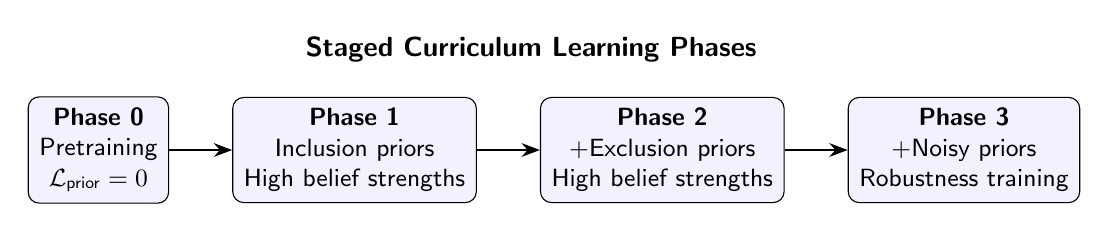
\begin{tikzpicture}[
  node distance=8mm and 8mm,
  >=Stealth,
  every node/.style={font=\sffamily\small, align=center},
  phase/.style={draw, rounded corners, fill=blue!5, minimum width=16mm, minimum height=12mm, inner sep=4pt}
]

% Phase 0
\node[phase] (P0) {\textbf{Phase 0}\\Pretraining\\ $\mathcal{L}_{\text{prior}}=0$};

% Phase 1
\node[phase, right=of P0] (P1) {\textbf{Phase 1}\\Inclusion priors\\High belief strengths};

% Phase 2
\node[phase, right=of P1] (P2) {\textbf{Phase 2}\\+Exclusion priors\\High belief strengths};

% Phase 3
\node[phase, right=of P2] (P3) {\textbf{Phase 3}\\+Noisy priors\\Robustness training};

% Arrows
\draw[->, thick] (P0) -- (P1);
\draw[->, thick] (P1) -- (P2);
\draw[->, thick] (P2) -- (P3);

% Title above
\node[font=\sffamily\bfseries, 
      above=10mm of $(P0)!0.5!(P3)$] 
      {Staged Curriculum Learning Phases};

\end{tikzpicture}
\vspace{0.5em}
\caption{Overview of the proposed staged curriculum learning procedure. Training begins in Phase 0 with no prior knowledge, followed by gradually introducing true priors (Phase 1), exclusion priors (Phase 2), and noisy priors (Phase 3). Each stage builds on the model trained in the previous one, ensuring a smooth transition from data-only, learning to robust prior-informed causal discovery.}
\label{fig:staged-curriculum}
\end{figure}

Our curriculum learning strategy is based around 4 distinct training phases. Each of these staged phases aim to progressively refine the model's ability to leverage prior knowledge with varying belief strengths. For each Phase \(i\), training begins using the pre-trained models of Phase \(i-1\), apart from Phase 0 in which the model is trained from scratch. An overview of the process is shown in Figure \ref{fig:staged-curriculum}.

\paragraph{Phase 0 - Pretraining (Data-Only Learning).}
The first stage, which we denote as Phase 0, establishes the foundation of the curriculum. At this point, the model is trained exclusively on the observational and interventional data without any form of prior knowledge. All prior-related inputs, such as prior tensors and belief strengths, are initialized to zero, resulting in the prior knowledge loss term vanishing, i.e., \( \mathcal{L}_{\text{prior}} = 0 \). This ensures that the model develops a baseline representation and learns to capture causal dependencies solely from the raw data. Importantly, although priors are not yet informative, the model architecture is already adapted to handle the additional input dimensions reserved for priors, thereby avoiding any architectural mismatch when subsequent phases introduce prior information. In this sense, Phase 0 provides a clean initialization point for the following stages.

\paragraph{Phase 1 - Incorporating Inclusion Priors.}
Once the baseline is established, we gradually expose the model to informative priors in Phase 1. Specifically, we sample a subset of ground-truth causal relations (edges or paths that exist) and inject them into the model as prior signals. These are provided with high belief strengths, drawn from the interval \(\mathcal{B}_{ji\mathcal{l}}\) sampled from \(\mathcal{U}(0.7,1)\), reflecting strong confidence in their correctness. By combining the learned representations from Phase 0 with these informative signals, the model is encouraged to align its predictions with reliable causal structures. To balance the contributions of different objectives, we set the binary cross-entropy edge classification loss coefficient to \(1.0\) and the prior knowledge loss coefficient to \(0.5\). This weighting scheme ensures that while prior knowledge influences training, it does not dominate the optimization, allowing the model to maintain flexibility in adapting to data

\paragraph{Phase 2 - Introducing Exclusion Priors.}
After the model has successfully integrated inclusion priors, Phase 2 introduces exclusion priors, i.e., the absence of certain causal edges. These are likewise injected with high belief strengths \( \mathcal{U}(0.7, 1)\), serving as strong negative examples. From an optimization perspective, this phase provides an additional form of regularization by pruning spurious dependencies the model might otherwise overfit to. The same loss weighting strategy as in Phase 1 is maintained, striking a balance between edge classification accuracy and prior consistency. Taken together, Phases 1 and 2 guide the model through a stage of “structured learning,” where it learns to incorporate both positive and negative causal evidence into its reasoning.

\paragraph{Phase 3 - Robustness to Noisy Priors.}
The final stage of the curriculum, Phase 3, aims to ensure robustness to imperfect prior knowledge. In practical applications, domain knowledge is often noisy, incomplete, or even contradictory. To prepare the model for such scenarios, we deliberately introduce noisy priors that include both wrong inclusions  and false exclusions, drawn with varying belief strengths. Unlike earlier stages, where priors served primarily as reliable guidance, this phase trains the model to weigh prior information against the data more critically. To avoid model collapse, learning rate is halved during this stage. By exposing the model to uncertainty and potential misinformation, Phase 3 acts as a robustness training stage, preventing overreliance on priors and encouraging adaptive integration of knowledge and evidence. This is particularly important in large-scale causal discovery settings, where domain knowledge may be abundant but not uniformly reliable.

























%\subsection{Random Prior Knowledge Sampling}
%
%We now refer to the methodology for obtaining edges/paths from the given ground truth graph and a paired belief strength tensor during training. For each causal graph in each training datch, we extract paths according to \textsc{FINDPATHS}, as described in Algorithm \ref{alg:find-paths}. 
%
%In brief, the algorithm unrolls the time-lagged causal graph and performs depth-first search (DFS) to extract all valid paths of length \(L\). We consider paths up to length \(\ell_{\max}\). It enumerates all directed causal paths up to a given maximum length \(L\) bounded by \(\ell_{\max}\) within a lagged adjacency tensor \( \mathbb{A} \in \mathbb{R}^{V_{\max} \times V_{\max} \times \ell_{\max}}\). Each directed edge \((i \rightarrow j, \ell)\) is considered active whenever \( \mathbb{A}_{ji\ell} > 0 \), indicating a positive influence from variable \(V^i\) to \(V^j\) at lag \(\ell\). From there, the ground truth lagged causal graph is initially binarized. Starting from every variable, a depth-first search (DFS) traversal unrolls the graph by expanding all active outgoing edges iteratively, thereby constructing all acyclic causal paths of length up to \(L\). In our implementation, cycles are being avoided, although the forward in-time nature of the causal graph does not preclude cycles. During traversal, the algorithm maintains a Boolean accumulator that encodes the validity of a partial path. This accumulator is updated multiplicatively as follows
%
%\begin{equation}
%\texttt{strength} \leftarrow \texttt{strength} \times \mathbf{1}[\mathcal{Y}[v,u,\ell] > 0]
%\end{equation}
%
%ensuring that only paths for which all constituent edges are active are retained. Formally, a valid causal path
%
%\begin{equation}
%\pi = {(u_t, u_{t+1}, \ell_t)}*{t=1}^{m}
%\end{equation}
%
%is included in the output if and only if
%
%\begin{equation}
%\prod*{t=1}^{m} \mathbf{1}[\mathcal{Y}[u_{t+1}, u_t, \ell_t] > 0] > 0.
%\end{equation}
%
%The algorithm returns a list of dictionaries, each describing a valid path with its ordered node sequence, corresponding lag values, and the terminal edge \((i,j,\ell)\). These extracted paths are later used for sampling and constructing prior-knowledge tensors in the training pipeline when accounting for prior knowledge.
%
%\begin{algorithm}[h!]
%\caption{Path Extraction in Temporal Causal Graph (FINDPATHS)}
%\label{alg:find-paths}
%\begin{algorithmic}[1]
%\renewcommand{\algorithmicrequire}{\textbf{Input:}}
%\renewcommand{\algorithmicensure}{\textbf{Output:}}
%\REQUIRE Lagged adjacency tensor $\mathcal{Y} \in \mathbb{R}^{V \times V \times \ell_{\max}}$, maximum path length $L$
%\ENSURE Set of valid paths $\mathcal{P}$ (each with \texttt{nodes}, \texttt{lags}, and \texttt{last\_edge})
%\STATE Initialize edge map $\texttt{edges} \gets \emptyset$
%\FOR{each $(i,j,k)$ with $\mathcal{Y}[j,i,k] > 0$}
%    \STATE $\ell \gets \ell_{\max} - k$
%    \STATE Append $(j,\ell)$ to $\texttt{edges}[i]$
%\ENDFOR
%\STATE $\texttt{paths} \gets \emptyset$
%\FOR{$s = 1$ to $V$}
%    \STATE $\texttt{stack} \gets [([s], [], 0, 1.0)]$ \COMMENT{Each element: (nodes, lags, depth, strength)}
%    \WHILE{$\texttt{stack}$ not empty}
%        \STATE Pop $(\texttt{nodes}, \texttt{lags}, \texttt{depth}, \texttt{strength})$
%        \STATE $u \gets \texttt{nodes}[-1]$
%        \IF{$u \notin \texttt{edges}$}
%            \STATE \textbf{continue}
%        \ENDIF
%        \FOR{each $(v, \ell) \in \texttt{edges}[u]$}
%            \IF{$v \in \texttt{nodes}$}
%                \STATE \textbf{continue} \COMMENT{Avoid cycles}
%            \ENDIF
%            \STATE $\texttt{new\_nodes} \gets \texttt{nodes} + [v]$
%            \STATE $\texttt{new\_lags} \gets \texttt{lags} + [\ell]$
%            \STATE $\texttt{new\_strength} \gets \texttt{strength} \times \mathbf{1}[\mathcal{Y}[v,u,\ell_{\max}-\ell] > 0]$
%            \IF{$|\texttt{new\_nodes}| \geq 2$ and $\texttt{new\_strength} > 0$}
%                \STATE Append $\{\texttt{nodes}=\texttt{new\_nodes}, \texttt{lags}=\texttt{new\_lags}, \texttt{last\_edge}=(u,v,\ell)\}$ to $\texttt{paths}$
%            \ENDIF
%            \IF{$\texttt{depth} + 1 < L$}
%                \STATE Push $(\texttt{new\_nodes}, \texttt{new\_lags}, \texttt{depth}+1, \texttt{new\_strength})$ onto $\texttt{stack}$
%            \ENDIF
%        \ENDFOR
%    \ENDWHILE
%\ENDFOR
%\RETURN $\texttt{paths}$
%\end{algorithmic}
%\end{algorithm}



	%\chapter{Results} \label{chap:results}

\begin{chapquote}{\textit{Thomas Huxley}}
``The great tragedy of science is the slaying of a beautiful hypothesis by an ugly fact.''
\end{chapquote}

This chapter contains the main experimental findings and results of LCMs. Section \ref{sec:exp-setup} elaborates on the experimental setup for assessing the performance of trained models. Section \ref{sec:metrics} is dedicated to the definition of the evaluation metrics for LCMs, while Section \ref{sec:baselines} contains the selection and description of established benchmarks. Section \ref{sec:ablations} concerns low to medium-scale results of ablation studies, while Section \ref{sec:res-lcms} covers results of large-scale LCMs. Trained models are evaluated on various dataset collections, both synthetic and simulated, as well as on in-distribution and out-of-distribution settings.


\section{Evaluation Setup} \label{sec:exp-setup}

Our evaluation setup can be briefly described as follows: We generate data collections as described in Chapter \ref{chap:data}, train LCMs with varying capabilities as described in Chapter \ref{chap:architecture} and using a training protocol as in Chapter \ref{chap:training}. We assess their predictive capabilities on various data collections, synthetic, semi-synthetic and simulated, both in-distribution and out-of-distribution, using performance metrics described in Section \ref{sec:metrics}.  

\section{Measuring Causal Discovery Performance} \label{sec:metrics}

We select standard metrics for predictive performance, as well as for causal graph distance. We evaluate the inferred lagged causal graph \(\hat{G}\) based on the presence and absence of directed edges compared to the ground truth lagged causal graph \(\mathcal{G}\). Recall that both the ground truth and inferred lagged causal graphs are padded both in the variable and lag dimension, so comparison is done on these padded graphs. Since causality is an asymmetric measure, and furthermore in the temporal case edges move forward in time, the directionality of an edge is taken into account.  We evaluate the learnt edges in terms of True Positives (TP), False Positives (FP), True Negatives (TN) and False Negatives (FN) \citep{sokolova2009systematic}. Ultimately, our comparisons revolve around the Area under the ROC curve (AUC) \citep{bradley1997use} metric, which is the reported metric in the main text. Their known definitions are applied, but for comparing the edges on the ground truth and inferred lagged causal graphs (Table \ref{tab:metrics}).

\begin{table}[ht!]
\centering
\caption{Definitions of evaluation metrics for binary predictions on learned causal graphs.}
\label{tab:metrics}
\begin{tabular}{ll}
\textbf{Metric} & \textbf{Definition} \\ \hline
TPR & Proportion of positives correctly identified. \\[6pt]
FPR & Proportion of negatives incorrectly identified as positives. \\[6pt]
TNR & Proportion of negatives correctly identified. \\[6pt]
FNR & Proportion of positives incorrectly identified as negatives. \\[6pt]
Precision & Proportion of positives correctly identified. \\[6pt]
Recall & Proportion of positives correctly identified. \\[6pt]
F1 & Harmonic mean of precision and recall. \\[6pt]
\textbf{AUC} & Area under the ROC curve (TPR vs. FPR) across different thresholds.
\end{tabular}
\end{table}

\par{TPR, FPR, TNR, FNR}. The \textit{True Positive Rate (TPR)} (also known as \textit{sensitivity}) measures the proportion of actual positives that are correctly identified by the model. \( \text{TPR} = \frac{TP}{TP + FN} \). The \textit{False Positive Rate (FPR)} measures the proportion of actual negatives that are incorrectly identified as positives, \( \text{FPR} = \frac{FP}{FP + TN} \). The \textit{True Negative Rate (TNR)} (also known as \textit{Specificity}), measures the proportion of actual negatives that are correctly identified as negatives, \( \text{TNR} = \frac{TN}{TN + FP} \). Finally, the \textit{False Negative Rate (FNR)} measures the proportion of true edges that are incorrectly identified as non-existent, \( \text{FNR} = \frac{FN}{FN + TP} \).

\par{Precision, Recall, F1}. We Additionally measure the \textit{Precision} (also known as \textit{Positive Predictive Value}) and \textit{Recall} (also known as \textit{Sensitivity}) metrics, which are defined as \(\text{Precision} = \frac{TP}{TP + FP}\), \(\text{Recall} = \frac{TP}{TP + FN}\) and \(\text{F1} = \frac{2 \cdot \text{Precision} \cdot \text{Recall}}{\text{Precision} + \text{Recall}}\). 

\par{AUC}. We measure the AUC (Area under ROC Curve) \citep{bradley1997use} using the area under the True Positive Rate and False Positive Rate at different prediction thresholds, based on the adjacency tensors of the ground truth and predicted DAGs. This is the same metric as the adjacency-based AUC introduced in Section \ref{sec:sim-results}, referred here simply as \(\mathrm{AUC}\). The predicted probabilities are obtained from the model and thresholded to \(\tau=0.05\), as well as the ground truth adjacencies (labels). Both time-lagged adjacency tensors are then flattened and concatenated along their batch dimension.

Figure \ref{fig:lagged-causal-graphs} depicts an example of a metric comparison between the ground truth and a possibly inferred output graph. 

\begin{figure}[t!]
\centering

% --- (a) Ground Truth ---
\begin{minipage}[t]{0.48\textwidth}
\centering
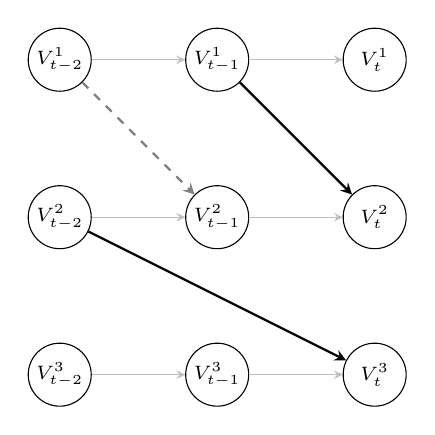
\begin{tikzpicture}[
    every node/.style={draw, circle, minimum size=0.8cm, font=\scriptsize, inner sep=0pt},
    >=stealth,
    ->,
    dashededge/.style={->, dashed, thick, color=gray},
    solidedge/.style={->, thick},
]

% t-2
\node (V1t2) at (0,4) {$V^1_{t-2}$};
\node (V2t2) at (0,2) {$V^2_{t-2}$};
\node (V3t2) at (0,0) {$V^3_{t-2}$};

% t-1
\node (V1t1) at (2,4) {$V^1_{t-1}$};
\node (V2t1) at (2,2) {$V^2_{t-1}$};
\node (V3t1) at (2,0) {$V^3_{t-1}$};

% t
\node (V1t) at (4,4) {$V^1_{t}$};
\node (V2t) at (4,2) {$V^2_{t}$};
\node (V3t) at (4,0) {$V^3_{t}$};

% Temporal arrows
\foreach \i in {1,2,3} {
  \draw[->, gray!50] (V\i t2) -- (V\i t1);
  \draw[->, gray!50] (V\i t1) -- (V\i t);
}

% Causal arrows (Ground truth)
\draw[solidedge] (V1t1) -- (V2t);
\draw[dashededge] (V1t2) -- (V2t1);
\draw[solidedge] (V2t2) -- (V3t);

\end{tikzpicture}

\vspace{0.3em}
{(a) Ground Truth}
\end{minipage}
\hfill
% --- (b) Inferred Graph ---
\begin{minipage}[t]{0.48\textwidth}
\centering
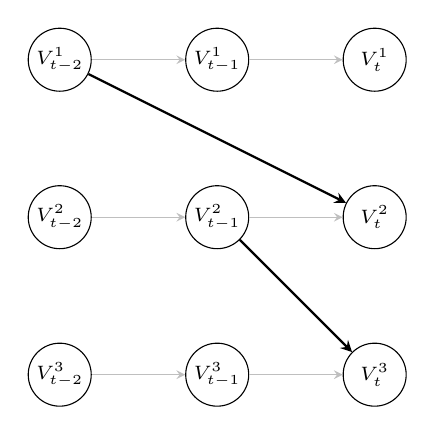
\begin{tikzpicture}[
    every node/.style={draw, circle, minimum size=0.8cm, font=\scriptsize, inner sep=0pt},
    >=stealth,
    ->,
    dashededge/.style={->, dashed, thick, color=gray},
    solidedge/.style={->, thick},
]

% t-2
\node (V1t2) at (0,4) {$V^1_{t-2}$};
\node (V2t2) at (0,2) {$V^2_{t-2}$};
\node (V3t2) at (0,0) {$V^3_{t-2}$};

% t-1
\node (V1t1) at (2,4) {$V^1_{t-1}$};
\node (V2t1) at (2,2) {$V^2_{t-1}$};
\node (V3t1) at (2,0) {$V^3_{t-1}$};

% t
\node (V1t) at (4,4) {$V^1_{t}$};
\node (V2t) at (4,2) {$V^2_{t}$};
\node (V3t) at (4,0) {$V^3_{t}$};

% Temporal arrows
\foreach \i in {1,2,3} {
  \draw[->, gray!50] (V\i t2) -- (V\i t1);
  \draw[->, gray!50] (V\i t1) -- (V\i t);
}

% Causal arrows (Inferred Example)
\draw[solidedge] (V1t2) -- (V2t);   % Wrong lag
\draw[solidedge] (V2t1) -- (V3t);   % Found one
% Missed edge: (V1t1 -> V2t)

\end{tikzpicture}

\vspace{0.3em}
{(b) Inferred Example}
\end{minipage}

\caption{Ground truth vs. inferred lagged causal graph with \(\ell_{\max}=2\) and \(3\) variables. Dashed edges encode causal stationarity, solid edges denote direct causal influence.}
\label{fig:lagged-causal-graphs}
\end{figure}

Although LCMs output a soft adjacency tensor \(\hat{\mathbb{A}}\) as discussed in Section \ref{sec:problem-formulation}, obtaining a binary causal graph from the soft predictions requires some sort of thresholding to the confidence scores. A thresholding operator is therefore defined, \(\hat{\mathcal{G}} = 1\{\hat{\mathbb{A}} \geq \tau\}\), with \(\tau\) either fixed (e.g., \(\tau = 0.05\)) or varied to compute ROC and AUC. Unless otherwise specified, reported results use \(\tau=0.05\). This procedure separates the training objective (which operates directly on soft predictions) from the evaluation protocol (which relies on binarized graphs). For threshold-independent comparisons, we sweep \(\tau\) to compute ROC and AUC.

\section{Comparison with Existing Approaches} \label{sec:baselines}

We compare the results of our framework with three other established works\footnote{For an overview on causal discovery algorithms, we refer the reader to the review paper by \citet{niu2024comprehensive}.} for temporal causal discovery: 

\begin{enumerate}

  \item The Peter-Clark Momentary Conditional Independence (\textit{PCMCI}) is a time-series causal discovery algorithm introduced by \cite{runge2018causal}. It is based on the constraint-based Peter-Clark (PC) algorithm by \cite{spirtes2001causation}, uncovering causal relationships using conditional independence tests of the form \( X_i(t-\tau) \rightarrow X_j(t) \) for lag \( \tau=0,\ldots,\ell_\text{max} \). The algorithm assumes the causal Markov condition, faithfulness, causal stationarity and causal sufficiency, while also accounting for contemporaneous (\(\tau=0\)) causation. The process consists of two phases, (i) the PC phase where, starting from a fully connected time-lagged graph up to lag \(\ell_\text{max}\) iteratively prunes spurious relationships by testing conditional independences, given a conditioning set and (ii) the MCI phase where, using Momentary Conditional Independence, tests for causal relationships while conditioning on both lagged and contemporaneous variables. Specifically, for each remaining candidate edge \(X^i_{t-\tau} \to X^j_t\), the Momentary Conditional Independence (MCI) test is performed, conditioning on both past and contemporaneous parents of \(X^j_t\) and parents of \(X^i_{t-\tau}\). This reduces false positives caused by autocorrelation and contemporaneous confounding, yielding higher precision in estimated causal graphs. In our implementations we use the official implementation of PCMCI, available in the \texttt{Tigramite} Python package. We select \(\alpha=0.05\) as the threshold of the adjacency matrix's p-values exclude contemporaneous edges, \( \ell_\text{max} = 3\). For independence tests we utilize partial correlation, which is estimated through a linear Ordinary Least Squares (OLS) regression and testing for non-zero linear Pearson correlation on the residuals and GPDC, which is a  conditional independence test based on Gaussian processes and distance correlation.

  \item \textit{DYNOTEARS} \citep{pamfil2020dynotears} is a time-series causal discovery algorithm, viewed as an extension of the NOTEARS \citep{zheng2018dags} method, which introduced causal discovery as a mathematical optimization problem with smooth acyclicity constraint. By leveraging the trace exponential function to enforce acyclicity and promoting sparsity using the \(\ell_1\) norm, this optimization program is solved using the augmented Lagrangian method, translating it into a series of unconstrained problems, in a similar setup to NOTEARS. Assuming \( M \) independent realizations of a \textit{stationary} time-series \( \left\{ x_{m,t} \right\}_{t=0}^{T} \) for \(\mathbf{x}_{m,t} \in \mathbb{R}^{d}\), the authors model the data using a Linear Structural Vector Autoregression (SVAR) model. The model is expressed as

  \begin{equation}
  \mathbf{x}_{m,t} = \mathbf{x}_{m,t}W + \sum_{i=1}^{p} \mathbf{x}_{m,t-i}A_i + \mathbf{z}_{m,t},
  \end{equation}

  where \(W\) represents contemporaneous (\textit{intra-slice}) dependencies, \(A_i\) lagged (\textit{inter-slice}) dependencies, and \( \mathbf{z}_{m,t} \) independent error terms. In matrix form this translates to,

  \begin{equation}
  \mathbf{X} = \mathbf{X}W + \mathbf{Y}A + \mathbf{Z},
  \end{equation}

  where \( \mathbf{X} \) contains the observations, \( \mathbf{Y} \) the time-lagged versions of \( \mathbf{X} \) and \( A \) is the concatenated matrix of lagged weights. The parameters of DYNOTEARS, apart from \( \ell_\text{max} \), are the regularization constants \(\lambda_\mathbf{W}, ~\lambda_{\mathbf{A}} \) that control the sparsity (as causal graphs are in general sparse), and the weight thresholds \(\tau_\mathbf{W}, ~\tau_{\mathbf{A}}\) that reduce the numerical error when computing \( h(\mathbf{W}) = \text{trace}(e^{\mathbf{W} \circ \mathbf{W}}) -d\). In our implementations, we select \(\lambda_{\mathbf{W}}=\lambda_{\mathbf{A}}=0.1\), thresholds \(\tau_\mathbf{W}=\tau_{\mathbf{A}}=0.05\), maximum number of iterations in the augmented Lagrangian method \(n=100\) and \(\ell_\text{max}=1\). Since DYNOTEARS' formulation is based on intra-slice and inter-slice dependencies for modeling the influence between variables in a contemporaneous and time-lagged setting respectively, we drop the contemporaneous predictions as we assume no contemporaneous effects in our experimental setup.

  \item \textit{VARLiNGAM} \citep{hyvarinen2010estimation} extends the LiNGAM (Linear Non-Gaussian Acyclic Model) to time-series data by integrating it with vector autoregressive (VAR) models and infers both lagged and contemporaneous causal relations, whereas the classic VAR only analyzes lagged causal relationships. Specifically, it estimates a Structural Vector Autoregression (SVAR) model of the form

  \begin{equation}
  \mathbf{x}(t) = \sum_{\tau=0}^{k} B_{\tau} \mathbf{x}(t-\tau) + \mathbf{e}(t),
  \end{equation}

  where \(B_\tau\) are \(n \times n\) coefficient matrices for lag \(\tau\), and \(\mathbf{e}(t)\) is a vector of mutually independent, non-Gaussian disturbances. The matrix \(B_0\) encodes instantaneous (contemporaneous) causal relations, while \(B_\tau, \, \tau>0\), encode lagged causal relations. 

  The key assumptions are: (i) linearity of the causal relations, (ii) non-Gaussianity and independence of disturbances, (iii) acyclicity of contemporaneous relations, and (iv) absence of latent confounders. Unlike Gaussian SVARs, where identifiability requires strong priors, VARLiNGAM leverages Independent Component Analysis (ICA) to achieve identifiability purely from statistical properties of the data. Estimation proceeds in two stages: first, autoregressive coefficients \(M_\tau\) are estimated via least squares; second, the residuals are subjected to LiNGAM analysis to recover instantaneous effects \(B_0\). The full causal matrices are then reconstructed as 
  
  \begin{equation}
  \hat{B}_\tau = (I - \hat{B}_0) \hat{M}_\tau, \quad \tau > 0
  \end{equation}

This yields a consistent estimator of both instantaneous and lagged effects. The authors show that neglecting \(B_0\) can severely bias lagged estimates, underscoring the importance of modeling contemporaneous effects.  In our experiments, we implement VARLiNGAM using the publicly available code and set \(\ell_\text{max}=3\), assuming first-order dependencies. Evaluation is restricted to lagged effects, discarding contemporaneous ones, in accordance with our experimental setup that excludes instantaneous causation.
 
\end{enumerate}

In addition to the above baselines, we also compare against the pre-trained Transformer model by \citet{stein2024embracing} on our 5-dimensional evaluation datasets.

\begin{algorithm}[t]
\caption{Bootstrap-based Estimation of Edge Probabilities} \label{alg:bootstrap}
\begin{algorithmic}[1]
\REQUIRE Time-series dataset $\mathcal{D}$, maximum lag $\ell_{\max}$, number of bootstraps $n$, causal discovery algorithm configuration $\mathbf{B}_\text{CD}$
\ENSURE Soft adjacency matrix $\mathbb{A} \in [0,1]^{V \times V \times \ell_{\max}}$

\STATE Initialize accumulator $\mathbf{S} \gets \mathbb{0}^{V \times V \times \ell_{\max}}$

\FOR{$b = 1$ to $n$}
    \STATE \COMMENT{Bootstrap Sampling Phase}
    \STATE Draw bootstrap sample $\mathcal{D}^{(b)}$ from $\mathcal{D}$ by resampling with replacement

    \STATE \COMMENT{Causal Discovery Phase}
    \STATE $\mathbf{A}^{(b)} \gets \text{causalAlg}(\mathcal{D}^{(b)}, \mathbf{B}_\text{CD})$

    \STATE \COMMENT{Edge Confidence Update}
    \STATE $\mathbf{S} \gets \mathbf{S} + f(\mathbf{A}^{(b)})$ 
    \STATE \COMMENT{$f$ extracts edge indicators or confidence scores}
\ENDFOR

\STATE \COMMENT{Normalization Phase}
\STATE $\mathbf{A} \gets \mathbf{S} / n$

\RETURN $\mathbf{A}$
\end{algorithmic}
\end{algorithm}

For all baselines, the official implementations are used or adapted, where needed, and the inferred graphs are transformed into a lagged adjacency form to ensure a fair comparison. The lag hyperparameter \(\ell_\text{max}\) is set precisely to that of our LCMs, i.e. \(\ell_\text{max}=3\). It should further be noted that not all methods output a lagged adjacency matrix of probabilities for edge existence (confidence scores) like our LCMs. For constraint-based methods like PCMCI, we use the inverse of the edge p-values as confidence scores, since the method outputs the p-values of the conditional independence tests for each lagged edge. For models that output an adjacency matrix of causal effect coefficients (like VARLiNGAM and DYNOTEARS), results are not directly comparable to our LCMs that output soft adjacency probabilities and computing AUCs is not directly applicable. For a fair comparison, we follow a bootstrap-based procedure to estimate the probability of each causal edge, as shown in the official documentation\footnote{\url{https://lingam.readthedocs.io/en/latest/tutorial/var.html}}. Specifically, we run both VARLiNGAM and DYNOTEARS \(n=10\) times with resampled datasets and compute the proportion of times each edge is discovered, resulting in a soft adjacency matrix of edge probabilities. Although computationally expensive, this approach allows for The pseudocode for this approach is shown in Algorithm \ref{alg:bootstrap}. 

To assess whether the differences in AUC scores between not only LCMs but benchmark methods as well are statistically significant, we employ the \textit{Wilcoxon signed-rank test}, a non-parametric paired test suitable for non-normally distributed data such as AUC scores. To control the family-wise error rate from multiple comparisons, we apply the \textit{Bonferroni correction} \(\alpha_\text{corrected} = \frac{\alpha}{k} \) where \(k\) is the number of pairwise comparisons. Additionally, each dataset instance is evaluated \(10\) times with different random seeds to obtain standard errors and confidence intervals. In the main text, the mean \(\mathrm{AUC}\) is reported (as defined in Section \ref{sec:metrics}) with standard errors. A complete list of experimental results is provided in the Appendix. 

\section{Ablation Studies} \label{sec:ablations}

\subsection{Ablation on Training Aid Techniques} \label{sec:ablation-training-aids}

In Chapters \ref{chap:architecture} and \ref{chap:training}, two approaches for enhancing the performance of LCMs were presented, as introduced by \citet{stein2024embracing}: \textit{Correlation Injection (CI)} (Subsection \ref{subsec:ci}) and \textit{Correlation Regularization (CR)} (Subsection \ref{subsec:cr}). The impact of both techniques is now quantitatively and thoroughly evaluated in terms of causal discovery performance, a gap that was previously unfilled. We report results for medium-sized LCMs (\(\approx 1\)M parameters) trained on the \texttt{S\_Joint} collection (Subsection \ref{subsec:data-training-synth}, Table \ref{tab:synthetic-datasets}) for in-distribution testing.

A baseline LCM was trained without any training aids, a second variant with CI only, and several models combining CI and CR with a grid search over the space of weight coefficients \(\lambda_{\text{CR}} \in \{0.25, 0.5, 0.75, 1.0\}\). The objective was two-fold: (i) to assess the relative contributions of CI and CR, and (ii) to identify a stable \(\lambda_{\text{CR}}\) value for subsequent large-scale experiments.

\begin{table}[h]
\centering
\caption{Ablation of training aids on \texttt{S\_Joint} (in-distribution). Statistical significance refers to improvement over the preceding variant, under a Bonferroni correction for multiple comparisons.}
\label{tab:training_aids_ablation}
\small
\begin{tabular}{lcc}
\toprule
\textbf{Model} & \textbf{AUC} & \textbf{Significant} \\
\midrule
LCM & 0.830 {\tiny $\pm$ .000} & -- \\
LCM + CI & 0.845 {\tiny $\pm$ .000} & Yes \\
LCM + CI + CR, ($\lambda_{CR}=0.25$) & 0.870 {\tiny $\pm$ .000} & Yes \\
LCM + CI + CR, ($\lambda_{CR}=0.5$) & 0.876 {\tiny $\pm$ .000} & Yes \\
LCM + CI + CR, ($\lambda_{CR}=0.75$) & 0.875 {\tiny $\pm$ .000} & No (vs 1.0) \\
LCM + CI + CR, ($\lambda_{CR}=1.0$) & 0.875 {\tiny $\pm$ .000} & No (vs 0.75) \\
\bottomrule
\end{tabular}
\end{table}

Table \ref{tab:training_aids_ablation} illustrates that both CI and CR substantially enhance causal discovery accuracy. CI alone provides a statistically significant improvement over the baseline (\(p < 10^{-7}\)), while the addition of CR further increases AUC across all tested regularization strengths. The highest mean AUC (\(0.876\)) is achieved for \(\lambda_{\text{CR}} \in [0.5, 0.75]\), with negligible variance.

A post-hoc significance analysis (Table \ref{app:training-aids-ablation-significance} in the Appendix) confirms no statistically significant difference between \(\lambda_{\text{CR}}=0.75\) and \(\lambda_{\text{CR}}=1.0\) (\(p=0.0192 > 0.01\), after correction), while all other pairwise comparisons remain significant. Consequently, \(\lambda_{\text{CR}}=0.75\) is adopted as the default configuration for subsequent large-scale experiments, balancing regularization strength and stability. Table \ref{app:training-aids-ablation} in the Appendix lists the full hyperparameter configuration and extended results.

\subsection{Optimal Mixture of Synthetic and Simulated Data} \label{sec:ablation-mixture}

To evaluate the optimal balance between purely synthetic and physically simulated training instances, we trained medium-sized LCMs (\(\approx 1\)M parameters) on varying mixtures of the two data sources. The synthetic datasets provide large-scale diversity and fundamental causal patterns, while simulated datasets (e.g., Kuramoto oscillators) introduce structured physical dynamics and noise realism. This experiment thus proves whether combining both data modalities enhances out-of-distribution (OOD) causal discovery, as findings from \citet{das2024decoder} illustrate, which also highlight the complementary role of synthetic and simulated data for generalization.

Models were trained on mixtures with synthetic-to-simulated ratios of 100/0, 80/20, 50/50, 20/80 and evaluated on the semi-synthetic \(\mathrm{Kuramoto}_5\) and Kuramoto benchmark collections. All runs used identical hyperparameters and incorporated both correlation injection and correlation regularization (\(\lambda_{\text{CR}} = 0.75\)).

\begin{table}[h!]
\centering
\caption{Out-of-distribution causal discovery performance (\(\mathrm{AUC}\)) of medium-sized LCMs trained on varying mixtures of synthetic and simulated data, evaluated on semi-synthetic Kuramoto benchmarks. Statistical significance refers to improvement over the preceding mixture, under a Bonferroni correction for multiple comparisons.} 
\label{tab:mixture_ablation}
\small
\renewcommand{\arraystretch}{1.15}
%\resizebox{\textwidth}{!}{
\begin{tabular}{lccc}
\toprule
\textbf{Mix (Synth / Sim)} & \textbf{AUC} (\scriptsize{\(\mathrm{Kuramoto_5}\)}) & \textbf{AUC} (\scriptsize{\(\mathrm{Kuramoto}\)}) & \textbf{Significant} \\
\midrule
100\% / 0\%  & 0.629 {\tiny $\pm$ .000} & 0.652 {\tiny $\pm$ .000} & -- \\
80\% / 20\%  & \textcolor{red}{\textbf{0.939}} {\tiny $\pm$ .000} & \textcolor{red}{\textbf{0.903}} {\tiny $\pm$ .000} & \textsc{Yes} (vs.\ 100/0) \\
50\% / 50\%  & 0.925 {\tiny $\pm$ .000} & 0.920 {\tiny $\pm$ .000} & \textsc{No} (vs.\ 80/20) \\
20\% / 80\%  & 0.872 {\tiny $\pm$ .000} & 0.922 {\tiny $\pm$ .000} & \textsc{No} (vs.\ 50/50) \\
\bottomrule
\end{tabular}
%}
\end{table}

Table \ref{tab:mixture_ablation} shows that training on purely synthetic data results in poor OOD performance (\(\text{AUC} < 0.65\)), reflecting overfitting to artificial data distributions. Adding a small proportion of simulated data (\(20\%\)) yields a dramatic increase in causal accuracy across both Kuramoto test sets (\(+0.27\)-\(+0.31\) AUC). Beyond this point, the effect plateaus, suggesting diminishing returns and a slight trade-off between generalization and over-regularization. The \(80/20\) mixture thus provides an optimal balance, achieving consistently high AUCs and statistical robustness across both benchmarks.

\begin{table}[t]
\centering
\caption{Out-of-distribution causal discovery performance (\(\mathrm{AUC}\)) of medium-sized LCMs trained on varying mixtures of synthetic and simulated data, evaluated on the \texttt{AirQualityMS} benchmark. Statistical significance refers to improvement over the preceding mixture, under a Bonferroni correction for multiple comparisons.}
\label{tab:airquality_mixture}
\small
\renewcommand{\arraystretch}{1.15}
\begin{tabular}{lcc}
\toprule
\textbf{Mix (Synth / Sim)} & \textbf{AUC} (\scriptsize{\(\mathrm{AirQualityMS}\)}) & \textbf{Significant} \\
\midrule
100\% / 0\% & 0.886 {\tiny $\pm$ .000} & -- \\
80\% / 20\% & \textcolor{red}{\textbf{0.957}} {\tiny $\pm$ .000} & \textsc{Yes} (vs.\ 100/0) \\
50\% / 50\% & 0.961 {\tiny $\pm$ .000} & \textsc{No} (vs.\ 80/20) \\
20\% / 80\% & 0.951 {\tiny $\pm$ .000} & \textsc{No} (vs.\ 50/50) \\
\bottomrule
\end{tabular}
\end{table}

Additionally, Table \ref{tab:airquality_mixture} shows that for \texttt{AirQualityMS}, adding a small proportion of simulated data \(20\%\) substantially improves OOD performance compared to purely synthetic training instances. However, increasing the fraction of simulated data beyond \(20\%\) does not yield statistically significant gains, which is also consistent with the Kuramoto benchmarks. These results reinforce the complementary nature of synthetic and simulated data: \textit{synthetic datasets enable efficient pretraining and coverage of structural variations, while simulated datasets enhance realism, stability, and transfer to real-world-like domains}. This hybrid strategy is adopted in all subsequent large-scale experiments. Additional results that support this finding are presented in the Appendix.

\section{Performance of Large-Scale LCMs} \label{sec:res-lcms}

This section evaluates large-scale LCMs, ranging from \(\sim\!2.5\)M to \(\sim\!24\)M parameters, on both in-distribution and out-of-distribution (OOD) causal discovery tasks. All models were trained with verified aiding techniques (CI and CR) and mixed synthetic-simulated datasets as described in Section \ref{sec:data-training}. While shallow models (\(\sim\)1M parameters) have already demonstrated strong generalization across higher-dimensional settings (up to 12 variables), this section investigates whether deeper models maintain or improve performance without degradation, a challenge previously observed by \citet{stein2024embracing}.  

\subsection{In-distribution Performance}

In-distribution generalization is evaluated on (i) the synthetic \texttt{S\_Joint} benchmark (3-5 variables) and (ii) the mixed \texttt{Synth\_230K\_Sim\_45K} holdout set of mixed synthetic-simulated data. The \texttt{S\_Joint} set additionally includes comparisons against the pretrained CP model from \citet{stein2024embracing}, which was trained on a similar small-scale synthetic distribution.

\begin{table}[h!]
\centering
\caption{In-distribution causal discovery performance (AUC) of large-scale LCMs and baselines.}
\label{tab:lcms_in_distribution}
\small
\renewcommand{\arraystretch}{1.15}
\begin{tabular}{lcc}
\toprule
\textbf{Model} & \textbf{S\_Joint (Synthetic)} & \textbf{Synth\_230K\_Sim\_45K (Holdout)} \\
\midrule
LCM-\texttt{2.5M} & 0.957 {\tiny $\pm$ .000} & 0.799 {\tiny $\pm$ .000} \\
LCM-\texttt{9.4M} & 0.962 {\tiny $\pm$ .000} & 0.800 {\tiny $\pm$ .000} \\
LCM-\texttt{12.2M} & 0.964 {\tiny $\pm$ .000} & 0.800 {\tiny $\pm$ .000} \\
LCM-\texttt{24M} & 0.936 {\tiny $\pm$ .000} & 0.800 {\tiny $\pm$ .000} \\
CP (Stein et al.) & 0.915 {\tiny $\pm$ .000} & -- \\
PCMCI & 0.672 {\tiny $\pm$ .000} & 0.783 {\tiny $\pm$ .000} \\
DYNOTEARS & 0.540 {\tiny $\pm$ .000} & 0.562 {\tiny $\pm$ .000} \\
VARLiNGAM & 0.801 {\tiny $\pm$ .000} & 0.773 {\tiny $\pm$ .000} \\
\bottomrule
\end{tabular}
\end{table}

\noindent
Table \ref{tab:lcms_in_distribution} illustrates that large-scale LCMs substantially outperform all classical baselines and maintain stable performance across scales.  
Despite the simplicity of \texttt{S\_Joint} (3-5 variables), the LCM-\texttt{12.2M} model achieves an AUC of \(0.964\), outperforming the CP model from \citet{stein2024embracing} which was explicitly trained on such data distributions, and at the same input dimensionality.  

In the mixed \texttt{Synth\_230K\_Sim\_45K} holdout test set, which combines synthetic and simulated data, LCMs achieve consistent AUC values around \(0.80\), confirming stable in-distribution generalization without any overfitting to training dynamics. This suggests that higher-capacity LCMs leverage their scale effectively when coupled with high-quality training data, as well as correlation-based injection \& regularization.

\subsection{Out-of-distribution / Zero-shot Performance}

We next test zero-shot transfer on three distinct OOD domains: semi-synthetic Kuramoto networks, \(f\)MRI-derived datasets (\(f\text{MRI\_5}\)), and the real-world AirQualityMS dataset, which is unseen during training and created using the ACT method (Section \ref{sec:data-simulated}).

\begin{table*}[h!]
\centering
\caption{Out-of-distribution (zero-shot) causal discovery performance (AUC) of large-scale LCMs and baselines across semi-synthetic and realistic benchmarks.}
\label{tab:lcms_ood}
\small
\renewcommand{\arraystretch}{1.15}
\begin{tabular}{lcccc}
\toprule
\textbf{Model} & \textbf{Kuramoto} & \textbf{\(f\)MRI\_5} & \textbf{AirQualityMS} & \textbf{Mean (OOD)} \\
\midrule
LCM-\texttt{2.5M} & 0.896 {\tiny $\pm$ .000} & 0.945 {\tiny $\pm$ .000} & 0.955 {\tiny $\pm$ .000} & 0.932 \\
LCM-\texttt{9.4M} & 0.926 {\tiny $\pm$ .000} & 0.943 {\tiny $\pm$ .001} & 0.914 {\tiny $\pm$ .001} & 0.928 \\
LCM-\texttt{12.2M} & 0.902 {\tiny $\pm$ .000} & 0.946 {\tiny $\pm$ .000} & 0.914 {\tiny $\pm$ .001} & 0.921 \\
LCM-\texttt{24M} & 0.913 {\tiny $\pm$ .000} & 0.954 {\tiny $\pm$ .000} & 0.813 {\tiny $\pm$ .006} & 0.893 \\
CP (Stein et al.) & -- & 0.775 {\tiny $\pm$ .001} & -- & -- \\
PCMCI & 0.640 {\tiny $\pm$ .000} & 0.739 {\tiny $\pm$ .005} & 0.556 {\tiny $\pm$ .000} & 0.645 \\
DYNOTEARS & 0.503 {\tiny $\pm$ .000} & 0.522 {\tiny $\pm$ .011} & 0.694 {\tiny $\pm$ .000} & 0.573 \\
VARLiNGAM & 0.584 {\tiny $\pm$ .000} & 0.687 {\tiny $\pm$ .005} & 0.552 {\tiny $\pm$ .000} & 0.608 \\
\bottomrule
\end{tabular}
\end{table*}

\noindent
Table \ref{tab:lcms_ood} demonstrates that large-scale LCMs achieve robust OOD transfer across diverse domains. While traditional temporal CD baselines (PCMCI, DYNOTEARS, VARLiNGAM) exhibit severe degradation, LCMs consistently exceed \(0.90\) AUC on all benchmarks. Notably, the LCM-\texttt{9.4M} and LCM-\texttt{12.2M} variants provide the most balanced trade-off between model scale and generalization, outperforming all baselines by wide margins.

Consequently, high-quality mixed training data, combined with correlation-based aiding techniques, enables LCMs to scale efficiently to higher dimensions without degradation. In both in-distribution and OOD regimes, the introduced models maintain or improve performance as capacity increases, demonstrating effective scaling behavior and robust generalization.

\section{Running Times} \label{sec:running-times}

This section provides a comparison of running times for various LCM variants. The fact that all pre-trained models operate on constant time complexity per sample is highlighted, in contrast to scaling issues present when fitting classic causal discovery algorithms, based on a one-model-per-dataset basis (Section \ref{sec:motivation}).

\begin{figure}[t]
\centering
\vspace{1em}
\includegraphics[width=\textwidth]{images/runtimes/running_times_synth_230k.png}
\caption{Running times on the \texttt{Synth\_230K} dataset (in-distribution, synthetic, holdout): Mean, standard deviation, and range across model variants and baselines. All trained models achieve superior running times compared to non-foundation model baselines.}
\label{fig:synth230k-runtimes}
\vspace{1em}
\end{figure}

Figure \ref{fig:synth230k-runtimes} shows the running times for the Synth\_230K dataset, highlighting the fact that LCMs are faster than other baselines (e.g., PCMCI, DYNOTEARS), even for deeper architectures. Numerical results are provided in Table \ref{tab:runtime-comparison}. To ensure a fair comparison, all models and baselines have been evaluated on a consumer-grade, 6-core, 12-thread CPU. Additional boxplots on running times are provided in the Appendix (Figures \ref{app:synth230k-runtimes} to \ref{app:kuramoto-10-runtimes}).

\begin{table}[h!]
    \centering
    \caption{Mean, minimum, and maximum elapsed time (in seconds) for trained LCMs in the \texttt{Synth\_230K} dataset (in-distribution, synthetic, holdout). All trained models achieve superior running times compared to non-foundation model baselines.}
    \label{tab:runtime-comparison}
    \vspace{0.5em}
    \begin{tabular}{lccc}
        \toprule
        \textbf{Model} & \textbf{Mean $\pm$ Std.} & \textbf{Range (s)} \\
        \midrule
        LCM 2.5M  & 0.014 $\pm$ 0.001 & (0.012, 0.047) \\
        LCM 9.4M  & 0.027 $\pm$ 0.002 & (0.023, 0.086) \\
        LCM 12.2M & 0.030 $\pm$ 0.003 & (0.026, 0.124) \\
        LCM 24M   & 0.041 $\pm$ 0.004 & (0.036, 0.100) \\
        PCMCI     & 0.749 $\pm$ 0.056 & (0.596, 1.453) \\
        DYNOTEARS & 0.264 $\pm$ 0.274 & (0.020, 4.532) \\
        VARLINGAM & 3.825 $\pm$ 0.327 & (2.567, 5.032) \\
        \bottomrule
    \end{tabular}
\end{table}


\section{Preliminary Results on Interventional Data} \label{sec:interventional-results}

To examine the direct impact of interventional samples on causal identifiability, we trained a medium-sized LCM (\(\sim\)2M parameters) as in Subsection \ref{subsec:scope-interventions}, but \emph{without} correlation injection (CI) or correlation regularization (CR) terms. This design isolates the effect of interventional information itself, avoiding auxiliary inductive biases that could otherwise obscure its contribution.

Training was conducted on a synthetic dataset of 40K sample pairs generated as per Section \ref{sec:data-synthetic}, with an 80/10/10\% split for training, validation, and testing respectively. Interventional samples were generated by random do-operations on either single or multiple interventional targets at each timestep, in accordance with the methodology outlined in Section \ref{sec:data-interventions}.

\begin{table}[h!]
    \centering
    \caption{Preliminary causal discovery results on synthetic data of a medium-size model (\(\sim\)2M parameters) with and without interventional samples, rounded to three decimal places.}
    \label{tab:interventional-results}
    \renewcommand{\arraystretch}{1.15}
    \small
    \begin{tabular}{lc}
        \toprule
        \textbf{Training Configuration} & \textbf{AUC} \\
        \midrule
        Observational data only & 0.742 \\
        Observational + Interventional data & 0.805 \\
        \bottomrule
    \end{tabular}
\end{table}

Table \ref{tab:interventional-results} shows that the inclusion of interventional data improves causal edge recovery. This result highlights that the observed gain in performance originates purely from the additional interventional signal rather than any imposed structural priors.

These preliminary findings suggest that LCMs can effectively incorporate interventional data to enhance causal identifiability. Future work aims to investigate whether this benefit persists under more complex hybrid observational-interventional scenarios and by comparing against different approaches.

\section{Preliminary Results on Prior Knowledge} \label{sec:prior-results}

This section investigates how the inclusion of prior causal knowledge and its associated belief strength affect inference in LCMs. Experiments were conducted on the \texttt{S\_Joint} dataset using a medium-sized LCM (\(\approx 1.8\)M parameters) and trained under the staged curriculum learning schedule described in Section \ref{sec:staged-curriculum-learning}. Similarly, no correlation injection (CI) or correlation regularization (CR) terms were used to avoid auxiliary inductive biases. Both the training and evaluation phases used the same dataset split to ensure consistency, while varying only prior information.

Prior knowledge is incorporated following the mechanism described in Subsection \ref{subsec:scope-prior}, where belief strengths are represented as scalar confidence values associated with each prior edge/path or exclusion. Two belief regimes were evaluated: (i) \textit{Low belief}, where prior confidence values are uniformly sampled from \([0.1, 0.3]\) and (ii) \textit{High belief} where prior confidence values are uniformly sampled from \([0.7, 0.9]\). These ranges align with the belief ranges used in the curriculum learning schedule defined in Section \ref{sec:staged-curriculum-learning}.

\begin{table}[h!]
    \centering
    \caption{Preliminary results on the effect of prior knowledge type and belief strength on causal discovery performance (AUC, rounded to two decimals) on the \texttt{S\_Joint} dataset. Performance against the same model without any prior knowledge and the observationally trained model from stage 0 of training is also reported.}
    \label{tab:prior-results}
    \renewcommand{\arraystretch}{1.15}
    \small
    \begin{tabular}{lcc}
        \toprule
        \textbf{Prior Type} & \textbf{Belief Strength} & \textbf{AUC} \\
        \midrule
        True Edge Priors & Low & 0.93 \\
        True Edge Priors & High & 0.96 \\
        Path Exclusions & Low & 0.91 \\
        Path Exclusions & High & 0.92 \\
        False Edge Priors & Low & 0.93 \\
        False Edge Priors & High & 0.89 \\
        All Types Combined & Low & 0.90 \\
        All Types Combined & High & 0.92 \\
        \midrule
        No Priors (same model) & - & 0.78 \\
        No Priors (weights from stage 0) & - & 0.74 \\
        \bottomrule
    \end{tabular}
\end{table}

Table \ref{tab:prior-results} shows that the presence of accurate priors enhances causal discovery accuracy, while incorrect priors or path exclusions can degrade performance. Importantly, the magnitude of these effects scales with the model's belief strength. High-confidence priors amplify both benefits and risks, improving results when priors are correct, but substantially reducing accuracy when priors are false, as evident by the depicted drop in AUC. 

Table \ref{tab:prior-results} reports our preliminary findings on the efficacy of prior knowledge in LCMs. Empirically, the inclusion of correct priors yields the highest AUC, confirming that informative priors improve causal discovery. Importantly, introducing false or contradictory priors only marginally reduces performance, indicating that the LCM succesfully integrates prior information in a stochastic and belief-weighted manner, rather than enforcing it deterministically. Compared to non-prior baselines (AUCs of 0.78 and 0.74 for the same model without priors\footnote{Prior knowledge and belief tensors given as zero tensors to the input.} and the observationally trained model from stage 0 of training\footnote{The model from stage 0 of training is trained as per the staged curriculum learning schedule described in Section \ref{sec:staged-curriculum-learning}.}, respectively), even weak priors improve performance. This demonstrates that the LCM's prior loss operates as a soft regularizer which, weighted by belief strengths and combined with evidence, allows discounting of implausible causal relations, as intended. When all prior types are combined, performance remains high, suggesting that the model effectively reconciles mixed-quality priors, thus avoiding implausible ones while leveraging consistent cues. The above observations highlight encouraging features for leveraging LCMs in real-world settings where expert knowledge is incomplete or unreliable. 
	%\chapter{Conclusion} \label{chap:conclusion}

\begin{chapquote}{\textit{Alan Kay}}
``The best way to predict the future is to invent it.''
\end{chapquote}

In this work, we introduced \textit{Large Causal Models} (LCMs), a family of foundation models for temporal causal discovery trained on large-scale datasets of time-series and corresponding ground-truth causal graphs. By leveraging a diverse mixture of synthetic and realistically generated datasets, our LCMs achieve strong generalization across domains and demonstrate competitive or superior performance to existing methods that require dataset-specific training, while operating in constant time, both at in-distribution and out-of-distribution scenarios.

\section{Summary of Contributions}

Our first research avenue focused on establishing a comprehensive data generation pipeline for causal discovery. We developed a scalable framework for sampling synthetic random temporal structural causal models (TSCMs), enabling the automatic generation of corresponding samples via ancestral sampling. In contrast to existing approaches that are limited in both generation diversity and expressivity, our framework supports the creation of hundreds of thousands of SCM instances with high variability and controlled complexity.

The second avenue addressed the integration of realistic datasets into training, aiming to increase model expressivity and predictive robustness. We referred to these datasets as simulated. Motivated by evidence that the inclusion of realistic data improves foundation model performance in out-of-distribution scenarios, we proposed a novel method, \textit{Temporal Causal-based Simulation (TCS)}, to bridge the gap between purely synthetic and real-world data. TCS enables the generation of thousands of causal models grounded in empirical data, paired with a Min-Max optimization scheme, \textit{Adversarial Causal Tuning (ACT)}, that facilitates optimal causal model selection. Together with subsampling across time and variable dimensions, it significantly expanded the available training corpus. Additionally, it serves as a method for benchmarking causal discovery algorithms, which is of vital importance in the Causality community.

Building on this foundation, the use of sample statistics within training and model inference was explored, showing that statistical regularization improves learning stability and performance. The integration of synthetic training data with realistic data was shown to improve generalization and robustness, demonstrating that causal foundation models also benefit from a diverse training corpus. Additionally, the current state-of-the-art has been extended from five to twelve input variables. In contrast to prior work trained solely on synthetic data and prone to performance degradation under scaling, introduced models maintain stable and robust behavior across both in-distribution and out-of-distribution settings, while surpassing or performing on par with established causal discovery algorithms.

Finally, a novel neural architecture for LCMs was proposed, integrating mechanisms such as patch-based representations and alternating attention layers. Early experiments indicate promising behavior, although these findings remain preliminary in nature. Initial explorations into the incorporation of interventional data and prior knowledge suggest potential avenues for extending foundation models for causal discovery towards a more unified scope.

Overall, this work aims to establish the conceptual and technical frame for scalable, foundation-style models in temporal causal discovery. Through a combination of training data generation, design and pretraining strategies, the groundwork for neural causal discovery methods that are robust, generalizable and applicable to complex real-world systems has been paved.

\section{Future Directions} \label{sec:future_work}

Our work regarding LCMs results in many interesting avenues for further research. Approaches for expanding our models may arise from reducing the amount of causal assumptions needed for interpreting the output of our models. For instance, by relaxing the assumption of causal sufficiency, explicit modeling of latent confounders (e.g., indirect causes such as \( X^i_{t} \leftarrow X^k_{t-1} \rightarrow X^j_{t}\)) is enabled, while the same can be done for the handling of contemporaneous effects. Another interesting point of research is to the inclusion of direct causal effects in the output of our LCMs. As causal effects are available during training from the ground truth causal graph, it would be interesting to investigate estimating them using an auxiliary task within the proposed framework. With the rise of AI Agents fine-tuned to specific tasks, we envision the incorporation of the output of LCMs into agents for causal discovery \textit{(Causal AI Agents)}. Such agents would actively reason about interventions, simulate outcomes, and refine their understanding of the environment through causal experimentation. By embedding LCMs as internal causal world models, such agents could autonomously generate and test causal hypotheses, while their natural language could serve as a natural medium for \textit{AI Explainability}.

While our LCMs present advances in scalable temporal causal discovery, they remain primarily a graph-predicting model, without explicitly modeling or leveraging disentangled, causal representations of the underlying processes. Recent work by \citet{scholkopf2021towards} highlights the potential of learning modular and invariant causal representations as a foundation for robust and generalizable reasoning. An exciting direction for future research would therefore be extending our LCMs to jointly learn structured representations that encode the independent mechanisms and interventions of the system, potentially improving interpretability and zero-shot generalization.

By bridging causal discovery, representation learning, and agentic decision-making, such systems could ultimately form the backbone of \textit{causally grounded AI}, a new paradigm where models not only predict correlations but understand and manipulate the causes that generate them.

\section{Epilogue \& Final Thoughts} \label{sec:epilogue}

%As this thesis comes to a close, it is tempting to view its pages as a finished story: Chapters written, contributions laid out, results measured and compared. Yet, like all stories in science, it is less an ending than a turning point; a comma rather than a full stop. 

Our journey began with a simple question: can we create a foundation model on the dance of time-series, to uncover the hidden strings of causality that govern examined data? How can this be achieved without the need for re-training on each independent data input? Along the way, we wandered through the importance of causal assumptions, the complexity of real-world data, and the black-box beauty of deep learning. Each of these contributions, felt at times like bricks in a cathedral still under construction: each one necessary, yet incomplete on its own. Together, they form a sturdy ground on which future contributions may build higher.

To this end, much remains to be explored. Questions left unanswered remain as important as those addressed. In the end, as large language models continue to rise in prominence, their limitations in causal reasoning highlight a parallel challenge: models that excel at pattern recognition but lack causal understanding risk producing contextually plausible yet logically unsound outputs. If causality is essential for LLMs, then LCMs represent an analogous step for temporal data: embedding causal reasoning at the very core of time-series modeling. \\

\begin{chapquote}{\citet{wu2024causality}}
``While LLMs excel at tasks involving language understanding, generation, and pattern recognition, they often struggle with tasks that require deeper causal reasoning. Without an understanding of causality, LLMs may produce outputs that are contextually relevant but not logically sound, leading to potential issues such as hallucinations, biased outputs, and an inability to perform well on decision-making tasks that depend on causal relationships. Incorporating causality into LLMs is essential for several reasons.''
\end{chapquote}

	\cleardoublepage
	\addcontentsline{toc}{chapter}{Bibliography}

	\nocite*{} % keep for now, remove later
	\bibliography{bibliography/thesis.bib}
		
	% Generate index (optional, if I'm using \makeindex)
	\cleardoublepage
	\printindex
	
\end{document}